% GLOBAL TODO LIST

% TODO: Fragezeichen suchen
% TODO: Proofread Kapitel 4 (Architekturen)
% TODO: schön machen

%\documentclass[pdftex,10pt,a4paper,twoside,openright]{scrreprt}
%\documentclass[pdftex,10pt,a4paper,twoside,openright]{scrbook} %12pt is offiziell
\documentclass[%pdftex,
	12pt,
	a4paper,
	twoside,
	%oneside,
	openright,
	parskip=half,   % Halbe Zeile Abstand zwischen Absätzen.
	headsepline,    % Linie nach Kopfzeile.
	footsepline,    % Linie vor Fusszeile.
	abstracton,     % Abstract Überschriften
	english        % Translator
	]{scrbook}
%\documentclass[10pt,a4paper]{report}

\usepackage[utf8x]{inputenc}
\usepackage{ucs}
\usepackage{amsmath}
%\usepackage{amsfonts}
\usepackage{amssymb}
\usepackage[xetex]{graphicx}
\usepackage{fontspec,xunicode}
\defaultfontfeatures{Mapping=tex-text,Scale=MatchLowercase}
\setmainfont{Calluna}
%\setsansfont{Helvetica Neue}
\setmonofont{Source Code Pro}
\usepackage{xltxtra}

% Glossar
\usepackage[
	nonumberlist, %keine Seitenzahlen anzeigen
	acronym,      %ein Abkürzungsverzeichnis erstellen
	%section,     %im Inhaltsverzeichnis auf section-Ebene erscheinen
	toc,          %Einträge im Inhaltsverzeichnis
]{glossaries}
%\usepackage{graphicx}
\usepackage{colortbl}
%\usepackage{url}
\usepackage{float}
\usepackage{color}
\usepackage{xcolor}
\usepackage{caption}
\usepackage{courier}
\usepackage[chapter,fontfamily=courier]{minted}
\usepackage[onehalfspacing]{setspace}
% Index-Erstellung
%\usepackage{makeidx}
\usepackage[scale=0.75]{geometry} % Um die Titelseite zu zentrieren
\usepackage[english]{babel}
\usepackage[babel,german=quotes]{csquotes}
% Spezielle Tabellenform fuer Deckblatt
\usepackage{longtable}
\usepackage{harvard}
% Fussnoten
\usepackage[perpage, hang, multiple, stable]{footmisc}
% Verschiedene Schriftarten

% Benutze die mylist-Umgebung, um nachher Hanging Bullets zu bekommen. Viel schöner :)
\usepackage{enumitem}
\newlist{mylist}{itemize}{1}
\setlist[mylist]{label=\textbullet,labelindent=-.5in,leftmargin=0pt,labelsep=.25in}

\usepackage{tocloft}

%\setlength\cftparskip{-2pt}
\setlength\cftbeforechapskip{2pt}


% bei two-side, da sonst paragraphen über die ganze seite gestreckt werden
\raggedbottom



\PassOptionsToPackage{hyphens}{url}
% PDF Einstellungen
\usepackage[%
	pdftitle={\pdftitel},
	pdfauthor={\autor},
	pdfsubject={\arbeit},
	pdfcreator={pdflatex, LaTeX with KOMA-Script},
	pdfpagemode=UseOutlines, % Beim Oeffnen Inhaltsverzeichnis anzeigen
	pdfdisplaydoctitle=true, % Dokumenttitel statt Dateiname anzeigen.
	pdflang=eng, % Sprache des Dokuments.
	pdflatex
]{hyperref}
\renewcommand{\UrlBreaks}{\do\/\do\a\do\b\do\c\do\d\do\e\do\f\do\g\do\h\do\i\do\j\do\k\do\l\do\m\do\n\do\o\do\p\do\q\do\r\do\s\do\t\do\u\do\v\do\w\do\x\do\y\do\z\do\A\do\B\do\C\do\D\do\E\do\F\do\G\do\H\do\I\do\J\do\K\do\L\do\M\do\N\do\O\do\P\do\Q\do\R\do\S\do\T\do\U\do\V\do\W\do\X\do\Y\do\Z}
% Colors
\definecolor{dunkelgrau}{rgb}{0.8,0.8,0.8}
\definecolor{hellgrau}{rgb}{0.95,0.95,0.95}
\definecolor{darkgray}{rgb}{0.8,0.8,0.8}
\definecolor{lightgray}{rgb}{0.95,0.95,0.95}
\definecolor{green}{rgb}{0.8,1.0,0.8}
\definecolor{red}{rgb}{1.0,0.8,0.8}
\definecolor{LinkColor}{rgb}{0,0,0.2}


% Placeholders
\newcommand{\titel}{The Paradigm Change from Thin to Rich Clients in Modern Web Applications
}
\newcommand{\autor}{Tim von Oldenburg}
\newcommand{\arbeit}{An analysis of how the MVC pattern is being shifted to the client side}
\newcommand{\matrikelnr}{0834311}
\newcommand{\kurs}{TIT09AIA}
\newcommand{\datumAbgabe}{September 2012}
\newcommand{\firma}{IBM Deutschland MBS GmbH}
\newcommand{\firmenort}{Herrenberg}
\newcommand{\abgabeort}{Stuttgart}
\newcommand{\abschluss}{Bachelor of Science}
\newcommand{\studiengang}{Applied Computer Science}
\newcommand{\dhbw}{Stuttgart}
\newcommand{\betreuer}{Daniel Suski} % evtl. mit Titel
\newcommand{\gutachter}{Paul Hubert Vossen} % evtl. mit Titel
\newcommand{\zeitraum}{12 Weeks}
\newcommand{\nexus}{{\acl{cn}}}
\newcommand{\ibm}{\ac{ibm}}

% Custom commands
\newcommand{\pathname}[1] {\sloppy{\texttt{\colorbox{lightgray}{#1}}}}
\newcommand{\code}[1] {\sloppy{\texttt{\colorbox{lightgray}{#1}}}}
\newcommand{\booktitle}[1] {``{#1}''}
\newcommand{\placeholder}[1] {{\color{red}#1}}
\newcommand{\fullref}[1] {\ref{#1}: \emph{\nameref{#1}}}

% Table rows have to be higher, too
\renewcommand{\arraystretch}{1.5}
\setlength{\tabcolsep}{10pt} %Abstand zwischen Spalten

% Redefinitions
\renewcommand{\labelitemi}{$\bullet$}
\renewcommand{\labelitemii}{$\cdot$}

% Widows and orphans
\clubpenalty=10000
\widowpenalty=10000
\displaywidowpenalty=10000

% Remove the point at the end of a description (glossary)
\renewcommand*{\glspostdescription}{}

%\renewcommand*{\lstlistlistingname}{List of Listings}

% Acronyms
\newcommand{\acs}[1] {\acrshort{#1}}
\newcommand{\acl}[1] {\acrlong{#1}}
\newcommand{\ac}[1] {\gls{#1}}
\newcommand{\acp}[1] {\glspl{#1}}

% (Farb-)einstellungen für die Links im PDF
\hypersetup{%
	colorlinks=false, % Aktivieren von farbigen Links im Dokument
	linkcolor=LinkColor, % Farbe festlegen
	citecolor=LinkColor,
	filecolor=LinkColor,
	menucolor=LinkColor,
	urlcolor=LinkColor,
	bookmarksnumbered=true % Überschriftsnummerierung im PDF Inhalt anzeigen.
}


\makeglossaries
% Acronyms

%\newacronym{rtc}{RTC}{Rational Team Concert\copyright}
%\newacronym{p8}{P8}{FileNet P8}
\newacronym{od}{OD}{OnDemand}
%\newacronym{cm}{CM}{ContentManager}
\newacronym{ear}{EAR}{Enterprise Archive}
\newacronym{jar}{JAR}{Java Archive}
\newacronym{war}{WAR}{Web Archive}

\newacronym{ica}{ICA}{IBM Content Analytics}

\newacronym{rad}{RAD}{Rational Application Developer}
\newacronym{was}{WAS}{WebSphere Application Server}
\newacronym{idx}{IDX}{IBM Dojo Extensions}
\newacronym{iis}{IIS}{Internet Information Services}

% Products
\newacronym{ide}{IDE}{Integrated Development Environment}
\newacronym{ecm}{ECM}{Enterprise Content Management}
\newacronym{cms}{CMS}{Content Management System}
\newacronym{icn}{ICN}{IBM Content Navigator}
\newacronym{cn}{ICN}{Content Navigator}
\newacronym{sccm}{SCCM}{SmartCloud Content Management}

% Patterns
\newacronym{mvc}{MVC}{Model--View--Controller}
\newacronym{mvvm}{MVVM}{Model--View--ViewModel}
\newacronym{mvp}{MVP}{Model--View--Presenter}
\newacronym{mv}{MV}{Model--View}

% Components
\newacronym{gui}{GUI}{Graphical User Interface}
\newacronym{ui}{UI}{User Interface}
\newacronym{api}{API}{Application Programming Interface}

% Technologies
% Server
\newacronym{http}{HTTP}{Hypertext Transfer Protocol}
\newacronym{tcp}{TCP}{Transmission Control Protocol}
\newacronym{asp}{ASP}{Active Server Pages}
\newacronym{php}{PHP}{PHP Hypertext Preprocessor}
\newacronym{jsp}{JSP}{JavaServer Pages}
\newacronym{cgi}{CGI}{Common Gateway Interface}
\newacronym{jee}{Java EE}{Java Platform, Enterprise Edition}
\newacronym{ejb}{EJB}{Enterprise JavaBeans}
\newacronym{url}{URL}{Uniform Resource Locator}
\newacronym{jre}{JRE}{Java Runtime Environment}
\newacronym{sql}{SQL}{Structured Query Language}
\newacronym{crud}{CRUD}{Create, Read, Update, Delete}
% Client
\newacronym{xml}{XML}{Extensible Markup Language}
\newacronym{json}{JSON}{JavaScript Object Notation}
\newacronym{html}{HTML}{Hypertext Markup Language}
\newacronym{css}{CSS}{Cascading Stylesheets}
\newacronym{js}{JS}{JavaScript}
\newacronym{dom}{DOM}{Document Object Model}
\newacronym{ajax}{AJAX}{Asynchronous JavaScript and XML}
\newacronym{amd}{AMD}{Asynchronous Module Definition}
\newacronym{ria}{RIA}{Rich Internet Application}

% Others
\newacronym{ietf}{IETF}{Internet Engineering Taskforce}
\newacronym{w3c}{W3C}{World Wide Web Consortium}
\newacronym{ibm}{IBM}{International Business Machines Corporation}
\newacronym{gps}{GPS}{Global Positioning System}
\newacronym{saas}{SaaS}{Software--as--a--Service}
\newacronym{paas}{PaaS}{Platform--as--a--Service}
\newacronym{iaas}{IaaS}{Infrastructure--as--a--Service}
\newacronym{io}{I/O}{Input/Output}
\newacronym{rest}{REST}{Representational State Transfer}
\newacronym{sso}{SSO}{Single Sign-On}
\newacronym{oop}{OOP}{Object-Oriented Programming}

% Glossary

\newglossaryentry{Taligent}
{
	name=Taligent,
	description={is an object-oriented operating system abandoned in the late 1990s}
}

\newglossaryentry{orwrapper}
{
	name=object-relational wrapper,
	description={is a software layer that maps objects in an object-oriented programming language to records in a relational database, for the purpose of persistence}
}

\newglossaryentry{oodb}
{
	name=object-oriented database,
	description={is a database that organizes data as objects and their references to each other, rather than in hierarchies or relations}
}

\newglossaryentry{rdb}
{
	name=relational database,
	description={is a database that organizes data in so-called relations, sometimes reffered to as tables}
}

\newglossaryentry{popup}
{
	name=popup window,
	description={}
}

\newglossaryentry{overlay}
{
	name=overlay window,
	description={}
}

\newglossaryentry{lazyloading}
{
	name=lazy loading,
	description={}
}

\newglossaryentry{timer}
{
	name=timer,
	description={or ``timer function'' is a programmatic function that gets executed in defined periods}
}

\newglossaryentry{p8}
{
	name=FileNet P8,
	description={or ``timer function'' is a programmatic function that gets executed in defined periods}
}

\newglossaryentry{cm}
{
	name=ContentManager,
	description={or ``timer function'' is a programmatic function that gets executed in defined periods}
}

% I have no idea what I'm doing...
\renewcommand\listoflistingscaption{List of Listings}



\begin{document}

\begin{titlepage}
	%\begin{longtable}{p{.55\textwidth} p{.85\textwidth}}
	%  {\includegraphics[height=1.6cm]{ibm.jpg}} & 
	%  {
\includegraphics[height=1.6cm]{dhbw.jpg}}
	%\end{longtable}
	\enlargethispage{20mm}
	\begin{center}
	  \vspace*{12mm}	{\LARGE\bf \titel }\\
	  \vspace*{12mm}	{\large\bf \arbeit}\\
	  \vspace*{12mm}	for the\\
	  \vspace*{3mm} 	{\bf \abschluss}\\
	  \vspace*{12mm}	in \studiengang\\
	  \vspace*{3mm} 	at the Baden--Wuerttemberg Cooperative State University \dhbw\\
	  \vspace*{12mm}	by\\
	  \vspace*{3mm} 	{\large\bf \autor}\\
	  \vspace*{12mm}	\datumAbgabe\\
	\end{center}
	\vfill
	\begin{spacing}{1.2}
	\begin{tabbing}
		mmmmmmmmmmmmmmmmmmmmmmmmmm     \= \kill
		\textbf{Time of Project}  \>  \zeitraum\\
		\textbf{Student ID, Course}  \>  \matrikelnr, \kurs\\
		\textbf{Company}      \>  \firma, \firmenort\\
		\textbf{Supervisor in the Company}              \>  \betreuer\\
		\textbf{Reviewer}             \>  \gutachter
	\end{tabbing}
	\end{spacing}
\end{titlepage}
\newpage
\thispagestyle{empty}
\mbox{}
\newpage
\thispagestyle{empty}
\mbox{}
\thispagestyle{empty}

\section*{Author's declaration}
% Seite 8
% http://studium.ba-bw.de/fileadmin/media/allgemein/bestimmungen/btechnik/richtlinien/Richtlinien_Praxismodule_Studien_und_Bachelorarbeiten_2011.pdf
\vspace*{2em}
Unless otherwise indicated in the text or references, or acknowledged above, this thesis is entirely the product of my own scholarly work. This thesis has not been submitted either in whole or part, for a degree at this or any other university or institution. This is to certify that the printed version is equivalent to the submitted electronic one.
\vspace{3em}

\abgabeort, \datumAbgabe
\vspace{4em}

\rule{6cm}{0.4pt}\\
\autor
\newpage
\thispagestyle{empty}
\mbox{}
%\newpage
%\clearpage



\chapter*{Abstract}
\thispagestyle{empty}
\begin{abstract}
The Model--View--Controller design pattern is used in many software
architectures to provide a
clear application structure. Following the principle of \emph{Separation of Concerns},
it decouples business data from business logic and presentation, and thus improves reusability and maintainability.
With the use of MVC in web applications,
the challenge emerges to apply the pattern to client--server environments.
The result of distributing the pattern components on client and server
is a range of different architecture variations.

%, are applicable for web applications following different requirements.

The applicability of these web architecture variations based on Model--View--Controller
is examined in this thesis by means of different application requirements.
To demonstrate the shift from thin to rich client web applications, the
architecture of \emph{IBM Content Navigator} is presented as an example.
The development of a plug--in for IBM Content Navigator further illustrates
how rich client MVC applications can effectively be implemented.

%By developing a plug--in for the rich client web application
%\emph{IBM Content Navigator}, a
\end{abstract}
\newpage
\thispagestyle{empty}
\mbox{}
\newpage
\pagenumbering{roman}
\setcounter{page}{1}
\printglossary[type=\acronymtype] % prints just the list of acronyms

%\clearpage
\newpage
\thispagestyle{empty}
\mbox{}

\makeatletter
\renewcommand{\@pnumwidth}{2.25em}
\renewcommand{\@tocrmarg}{2.25em}
\makeatother

\tableofcontents

%\newpage


\chapter{Introduction}
\label{chap:introduction}
\setcounter{page}{1}
\pagenumbering{arabic}
Consumer applications have existed on the web for more than a decade now. Amongst others, e-mail, time management, social collaboration and file sharing applications can all be accessed using a web browser. For consumers, the main advantages are the independence of special software and the ability to access their data from nearly any computer, but web applications are also an interesting approach for enterprise solutions: In opposition to desktop applications, web applications do not need to be installed on end-user machines. This advantage is complemented by the fact that the roll-out of updates can easily be performed on the server-side only.

Until recently, browsers were not powerful enough for desktop-level, complex end-user clients. But as rendering techniques and JavaScript engines get faster, the possibilities of \glspl{bba} grow. In combination with JavaScript frameworks, web browsers become a runtime environment, powerful enough to build applications that can replace traditional end-user clients.

The \acl{mvc} pattern is a commonly used architectural design pattern. Being based on the principle of \emph{Separation of Concerns}, it helps to structure an application by dividing it into three different parts: the Model, which holds business data, the View, which displays these data, and the Controller, which is responsible for user interaction.

MVC was created in the 1970s, long before the world wide web became popular, and has been used in many desktop applications since. But applying it to the domain of web applications introduces a challenge: the web is a distributed computing environment. While it is rather simple to connect MVC components inside a monolithic desktop application, distributing them across different tiers --- at least \emph{client} and \emph{server} --- opens up possibilities for different implementations. With respect to three defined criteria, this thesis investigates and evaluates different web application architectures based on the Model-View-Controller pattern.

\glsunset{ibm}
\glsunset{cn}
\section{Motivation and Scope}
In the following section, \emph{IBM Content Navigator}, one of IBM's most recent web clients, is introduced. By connecting it to \acl{ecm} and SmartCloud Content Management, the business problem that leads to the goals of this thesis is explained.

%\subsection*{Web Applications within IBM}
%The \ac{ibm} corporation has recognized the advantages that browser-based applications have for enterprise solutions. Several products of IBM are or are accompanied by web clients, such as \emph{Connections}\footnote{See \url{http://www-01.ibm.com/software/lotus/products/connections/}}, a social software for companies, or \emph{LotusLive}\footnote{See \url{https://www.ibm.com/cloud-computing/social/us/en/webmeetings/}}, a web meeting tool. IBM also builds software to create web applications, for example the IBM Web Experience Factory\footnote{See \url{http://www-01.ibm.com/software/genservers/webexperiencefactory/}}.

% Part of the company's long term strategy regarding web applications is \emph{The Dojo Toolkit}. Dojo is an open source JavaScript framework to build rich, client-side web experiences based on widgets and the \emph{AJAX} technique. It is used throughout IBM's web application portfolio. Recently\footnote{See \url{http://maqetta.org/index.php?view=article&catid=2&Itemid=9&id=28}}, IBM contributed \emph{Maqetta} as open source to the Dojo Foundation\footnote{The foundation is backing the development of Dojo.}. Maqetta is a visual authoring tool for creating HTML5 web applications based on Dojo.

%IBM provides guidelines to unify the User Experience\footnote{The look and feel of a \ac{ui}.} of web applications, known as \emph{OneUI}. There are also IBM internal extensions to Dojo that primarily enhance existing \glspl{widget}, called the \emph{\ac{idx}}.

\subsection*{Enterprise Content Management and IBM Content Navigator}
According to \citeasnoun{wiki:ecm}, ``\ac{ecm} is a formalized means of organizing and storing an organization's documents, and other content, that relate to the organization's processes. The term encompasses strategies, methods, and tools used throughout the lifecycle of the content.'' Contracts, invoices, orders or insurance policies are all examples for such content. IBM offers different solutions for \ac{ecm}, three of them being \glspl{repository} to manage digital documents: \emph{\gls{p8} (P8)}, \emph{\gls{cm} (CM)} and \emph{ContentManager OnDemand (OD)}. All three are complemented by web clients used to access the repositories (e.g. to upload, download, or move documents): \emph{Workplace XT} for FileNet and \emph{WEBi} for CM and OD. They are usually delivered with every solution that also includes their respective repository software.

%\ac{ibm} adresses \ac{ecm} with two solutions to manage digital documents: \emph{\gls{p8}} and \emph{\gls{cm}}. Both are complemented by web clients used to access the repositories (e.g. to upload, download, or move documents): \emph{Workplace XT} for FileNet and \emph{WEBi} for ContentManager.

Amongst other clients of IBM ECM products, Workplace XT and WEBi are going to be replaced by \ac{icn}\footnote{See \url{http://www-01.ibm.com/software/ecm/experience.html}}. This new web application allows access to FileNet, ContentManager and ContentManager OnDemand repositories through a single \acl{ui}. 
IBM Content Navigator is a Rich Client based on the \acl{mvc} pattern. It makes use of \emph{The Dojo Toolkit}, which is an open source JavaScript framework to build rich, client-side web experiences based on widgets and the \emph{AJAX} technique. Dojo is the standard framework used by most of the IBM web clients.
ICN follows IBM OneUI, which is an initiative within IBM to unify the user experience\footnote{The look and feel of a \acl{ui}.} in products' web clients by providing guidelines. Content Navigator also makes use of IBM internal extensions to Dojo, called the \emph{\acl{idx}}, which primarily enhance existing Dojo widgets to follow the OneUI standards.

%Built on the \acs{ajax} technique and \emph{The Dojo Toolkit}, and following the OneUI guidelines, Content Navigator is a Rich Client following the MVC pattern.

\begin{figure}[H]
	\centering
	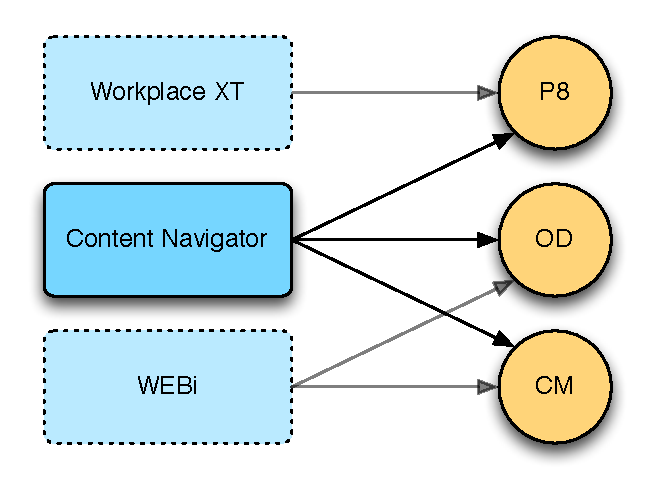
\includegraphics[width=10cm]{images/nexus.pdf}
	\caption{IBM Content Navigator replaces WEBi and Workplace XT}
	\label{fig:nexusp8cmod}
\end{figure}

Due to its plug-in based architecture, IBM Content Navigator can not only be used as a distinct application, but also as a framework which can be used to build arbitrary web applications. Although originally built with the access to ECM content repositories as a core feature, web applications developed on top of \ac{icn} can serve any purpose.

\nexus\ makes integration of different applications possible through two features:
\begin{itemize}
	\item A plug--in system that allows developers to create extensions for every purpose and on every layer with both server-side and client-side features
	\item A client-oriented \ac{mvc} architecture that provides the structure for the rich, browser-based application
\end{itemize}

\subsection*{SmartCloud Content Management}
IBM \ac{sccm} is a \ac{saas} offering for document and email compliance archiving. It is part of IBM's ECM portfolio and integrates different IBM products to deliver an out-of-the-box archiving solution for enterprises. One of these integrated products is the document management system \emph{FileNet P8} and its web client, \emph{Workplace XT}. In addition to Workplace XT, SCCM also provides a browser-based administration interface.

As Workplace XT is going to be replaced by \ac{icn}, it is planned to port the SCCM administration interface to the \ac{icn} platform for the next release, too. This integration will provide customers with a unified \acl{ui} for the different web clients delivered through SCCM.

\subsection*{Goals and Scope}
As a first goal, this thesis demonstrates how the \ac{mvc} pattern can best be implemented in web applications. Based on three defined criteria, different MVC-based web application architectures are evaluated to investigate the shift to rich, JavaScript-based clients.

The second goal of this thesis is to investigate and present the part of the IBM Content Navigator architecture related to the MVC pattern. In conjunction with the thesis of Robert Metzger, a working prototype of an ICN plug-in was developed to approach a problem being faced with the SCCM cloud offering. The plug-in demonstrates how the MVC pattern can be implemented in practice and should help the SCCM development team to get up to speed with porting the SCCM administration interface to IBM Content Navigator.

It is not in the scope of this thesis to create a new way to implement MVC in web applications. It is also neither a goal to find and list all possible implementations of MVC architecture on the web, nor to find the single best way to implement it. Instead, four MVC architectures and their applicability are compared to identify the one that best fulfills an application's requirements.
\newpage
\section{Document Structure}
\emph{Chapter One, ``\nameref{chap:introduction}''} explains the motivation behind this thesis. It familiarizes the reader with the business background, defines goals and outlines the document structure.

\emph{Chapter Two, ``\nameref{chap:mvc}''} introduces \acs{mvc}, its history and origins in \mbox{Smalltalk-80}, its structure and the tasks of the different components. It also presents two variations of \ac{mvc} --- MVP and MVVM --- which are commonly used in web applications.

\emph{Chapter Three, ``\nameref{chap:webapparch}''} describes technologies and techniques relevant to web application architecture and explains the terms \emph{Thin Client} and \emph{Rich Client}.

\emph{Chapter Four, ``\nameref{chap:webmvc}''} gives examples of problems that emerge with web applications and defines these problems as criteria. After that, various possibilities to implement \ac{mvc} in client--server architectures are discussed based on the previously defined criteria.

\emph{Chapter Five, ``\nameref{chap:nexus}''} presents \acl{icn} and examines its plug--in system and architecture. Hereafter, the design of a log analysis plug--in developed in the course of this thesis is discussed further.

\emph{Chapter Six, ``\nameref{chap:conclusion}''} summarizes the findings and gives an outlook on web application architecture with respect to current developments and evolving standards.
\chapter{The Model--View--Controller Pattern}
\label{chap:mvc}
This chapter discusses the \acl{mvc} pattern. It introduces design patterns in general, the classical \acl{mvc} architecture and different interpretations and variations of it.
\section{Design Patterns in Software Engineering}
The principle of using design patterns was first introduced by \citeasnoun{alexander}. The architects describe how a community can shape towns, neighbourhoods and buildings with simple tools. To communicate architectural knowledge in an effective way to the readers, he introduces \emph{design patterns}:
\begin{quote}
	\enquote{Each pattern describes a problem which occurs over and over again in our environment, and then describes the core to the solution to that problem, in such a way that you can use this solution a million times over, without ever doing it the same way twice.} \cite[p. 10]{alexander}
\end{quote}
This shows the main aspects of a design pattern:
\begin{enumerate}
	\item A pattern provides a solution to a specific, frequently occurring problem
	\item The pattern's solution is generic (only ``the core to the solution'', but no implementation details)
	\item The main advantage of a pattern is reusability
\end{enumerate}
Design patterns are a method of communicating solutions that have proven to solve a specific problem. Alexander's definition is open enough to be applied to nearly any field that deals with design problems, for example graphic design, architecture, interaction design, and software design. Most of these areas have repositories of design patterns. For architecture, there is the aforementioned book by Christopher Alexander, interaction design patterns can be found at the \emph{Yahoo! Design Pattern Library}\footnote{See \url{http://developer.yahoo.com/ypatterns/}}, and software design patterns are listed in the \emph{Portland Pattern Repository}\footnote{See \url{http://c2.com/ppr/}}.

\citeasnoun{gof} describe design patterns that are used in object-oriented software development. There are design patterns for other programming paradigms, but most of the more popular ones are created for object-orientation, especially as they leverage the given reusability that \acs{oop} provides through classes, interfaces, \glspl{prototype} or \glspl{mixin}.

Design Patterns simplify software development. If a pattern used in a software is well documented and understood, it is easier to maintain the software, to reuse code, and easier to communicate software architecture to new developers.

Gamma et al. classify the described design patterns into three categories, depending on their purpose.

\begin{description}
	\item[Creational Patterns] provide a way to create objects under certain circumstances (also known as \emph{object instantiation}).
	A popular example of creational patterns is the \emph{Singleton}, which ensures that only one instance of an object exists at a given time.
	\item[Structural Patterns] describe the composition (or \emph{structure}) of different objects or classes. They offer additional ways of composing as those already given through object-orientation (such as composition, aggregation or association). An example for a structural pattern is the \emph{Proxy}, which simulates the existence of a remote or otherwise unaccessible object by copying its interface and forwarding method calls. Amongst other purposes, proxies are used to simplify remote access or to realize access control.
	\item[Behavioral Patterns] are used to define the interaction of objects or classes, the flow of control or the distribution of responsibility. The \emph{Chain of Responsibility}, for example, is a sequence of interconnected objects that handle specific input. Depending on the type and content of this input, an element in the Chain of Responsibility may or may not process the input and pass it on to its successor.
\end{description}
According to \citeasnoun{gof}, design patterns exist on different levels of abstraction. The patterns described in \booktitle{Design Patterns} are mostly scoped on classes and objects. On a higher level of abstraction, there are \textbf{Architectural Patterns}\footnote{There are patterns of software architecture, not to be confused with the architecture patterns that \citeasnoun{alexander} described.}, one of them being \emph{\acl{mvc}}. Architectural patterns are not described by Gamma et al., but MVC in particular is mentioned as an illustrative example in the introductory chapter \citeyear[p. 4--6]{gof}. A collection of architectural patterns is listed by \citeasnoun{poeaa}.

%- Patterns are important to structure software
% compound: includes other patterns, such as publish-subscribe
% much interpreted, much misinterpreted
\section{History and Interpretation of MVC}
This section outlines the structure and control flow of \acl{mvc}. It explains the origins of MVC, describes the different components and discusses what leads to the different interpretations and variations of MVC.

\subsection{Origins of MVC in Smalltalk-80}
\acl{mvc} was first introduced by Trygve Reenskaug while he was working with the \gls{smalltalk} group at Xerox PARC from 1978 to 1979. He designed several versions that included the components ``Editor'' and ``Thing''\footnote{Editor and Thing are components that were part of very early versions of \ac{mvc}. They are not further discussed here.} before he settled on the MVC terminology. Reenskaug defined the MVC pattern for the use in applications with a \ac{gui}. His initial idea was to map the user's mental model of the data to the computational representation of the data. For this to achieve, he wanted to abstract the data, using different components and hiding the real Model from the user --- a principle that is called \emph{Separated Presentation}. Reenskaug summarized his work on \gls{mvc} in \booktitle{The Model--View--Controller (MVC). Its Past and Present}~\citeyear{reenskaug03}.

According to \citeasnoun[p. 99ff.]{osmani}, MVC takes the separation one step further and makes a clear division between the user interface and the application logic. This concept is now called --- more generally --- \emph{Separation of Concerns}. Before Smalltalk-80 MVC, Graphical User Interfaces were designed as one single module of code. This module handled the data, the presentation and the user interaction. While this worked well for tiny applications, it was hard to maintain for regular or large applications. Separating the presentation, user interaction (logic) and data allows to reuse these components.

\subsection{MVC Components}
Model, View and Controller are the components of a MVC architecture. Due to the high interpretability of this pattern, a common definition of the components and the pattern structure could not be found during research for this thesis. Thus, the definitions below are based on the different sources of Trygve Reenskaug, Gamma et al. and Martin Fowler.

\subsubsection{The Model}
MVC-based applications are data-centric, which means they are based on \emph{knowledge} that is organized in one or more \emph{Models}. A Model is the programmatic representation of these data, either the whole set or only a part.

Neither the characteristics of the data nor the way they are stored within the Model is relevant in this context. Data may be
\begin{itemize}
	\item \emph{structured}, such as a numerical table or a filled-out form
	\item \emph{semi-structured}, such as a XML or Microsoft Word document
	\item \emph{unstructured}, such as the body of an e-mail (free-form text).
\end{itemize}
A Model may store a particular element of its data in any way, depending on the data characteristics, the programming paradigm used and the requirements of the application. Possible storage models include, but are not restricted to
\begin{itemize}
	\item \emph{Objects} as used in object-oriented programming languages, such as Java objects or JavaScript objects
	\item \emph{Arrays} and \emph{Lists} as used in most programming languages
	\item \emph{Plain binary or textual streams} like files. A file system along with I/O functions can act as a Model.
\end{itemize}
Reenskaug described the original \ac{mvc} assuming Models would be Smalltalk objects, but with the spread of other programming languages and databases, every storage model can be imagined.

Often, Models contain more than just the plain data they embody. As is stated in \citeasnoun{reenskaug79a}, a Model is ``represented in the computer as a collection of data together with the methods necessary to process these data.'' This means, a Model can also contain functions, such as to \emph{create}, \emph{read}, \emph{update} and \emph{delete} data (also knows as \emph{\acs{crud}}). Auxiliary structures, such as hashes and indices, as well as functions add data-related business logic to the Model. They can simplify the handling of data extremely, for example through input validation, data conversion, sorting capabilities and faster access. % sollte business logic nur im controller sein? quelle?

A concept found in many collections of data, such as Java objects or relational databases, is the dependance of data on other data. A Java object, for example, can have the reference to a different object as one of its attribute values. In relational databases, a \gls{tuple} can refer to another tuple, which is part of either the same or a different \gls{relation}, using a foreign key. Those references have to be considered when designing Models.

In many cases, the data source is not the actual Model, depending on the point of view. If a Java application implementing \acl{mvc} needs to access data in a relational database, this is most probably implemented using an object-relational wrapper. From the point of view of the Java application, the wrapper classes are Models, while from an architectural point of view, the database (or the database tier) represents the Models. Such ambiguities lead to the need of good communication in the design and development teams, and they are one reason for the various interpretations of the pattern.

To clarify what the ``Model'' means in a given context --- for example, in one development team --- \citeasnoun{reenskaug79a} proposes that all Models should have the same level of abstraction. That means, ``Model'' should never describe a database and, at the same time, an object holding data from this database, which would be more concrete than the database itself and thus on a different level of abstraction.

\subsubsection{The View}
As MVC is a pattern for applications with a user interface, the View is responsible for (visual) data presentation. It can reach from a simple, textual representation to tables, charts and diagrams or even more complex output. A View is always connected to a Model and is used to present the Model's data. A View is usually related to one Model only, whereas a Model can have multiple Views.

The output medium according to \citeasnoun{reenskaug79a} is either the screen or hardcopy (print), but nowadays other output media, such as audio (for example a speech synthesizer) or haptics (for example a \emph{braille} device used by blind people to interact with a computer) can be applied to the View concept. However, in software development, the screen is still the main output device, and is focused on in this definition; therefore, the terms ``present'', ``show'' and ``display'' are used synonymously.

Usually, not all data of a Model are presented at once. There are two ways of limiting the presented data, both of which can be compared to relational algebra for illustration. On the one hand, a View can display only several chosen facets of the Model. This can be compared to a \emph{projection} in relational algebra. On the other hand, the set of data can be limited, so that only items that match certain criteria or not more than a specific number of items are displayed. This can be compared to a \emph{selection} in relational algebra.

As the View is an interface to the user, the functionality described above is needed in order to let the user focus on the important part of the data. Scrolling, pagination and lazy loading are all examples for features that support this functionality of the View component. \citeasnoun{reenskaug79b} calls the View a ``presentation filter''.

To fulfill the task of presenting a Model's data, a View has to know about the Model. (In contrast, the Model is totally independent of the View.) This knowledge is needed for two reasons: On the one hand, it needs to have access to the actual data to be able to display them. On the other hand, a View may need to know metadata to display the actual data properly.

To illustrate the latter, we can imagine a table (View) that displays data from a relational database (Model). Whereas some columns show text or numbers, another one displays dates which have to be formatted according to the user's local settings. This cannot be the Model's task; it is aware of the fact that this piece of data is a date, but it does not know how to format a date properly. This would be the task of the presentation component, which in \acl{mvc} is the View.

The data a View displays are held in the View's private buffer. When the Model changes, the View has to be informed about that to update these data. To fulfill this, the View is connected to the Model via an Observer pattern as described by \citeasnoun{gof} (see Section~\ref{sec:modelview} for more information on the Observer).

\subsubsection{The Controller}
The exact role of the Controller is probably the most discussed part of \acl{mvc}. The resulting variations, such as \acl{mvvm} or \acl{mvp} all kept the Model and View, but redefined what used to be the Controller. To clearly draw a picture of the Controller's task, Reenskaug's definition is taken into account:
\begin{quote}
	\enquote{A controller is the link between a user and the system. It provides the user with input by
	arranging for relevant views to present themselves in appropriate places on the screen. It
	provides means for user output by presenting the user with menus or other means of giving
	commands and data. The controller receives such user output, translates it into the appropriate
	messages and pass these messages on to one or more of the views.} \cite{reenskaug79b}
\end{quote}
In other words, the Controller is the part of an application that implements the overall application flow and the user interaction. As already mentioned, \acl{mvc} is an architectural pattern for applications with a \acl{gui}. The Controller processes user input, for example such input that is used to manipulate the Model.

Some interpretations add the term of an \emph{Application Controller} to pay respect to the fact that there are Controllers on different layers of the application, as described by \citeasnoun[pp. 379--386]{poeaa}. A View-bound Controller may react when the View is clicked, but it can only know that from a higher--level Application Controller that tracks mouse movements and events. In the case of web applications, this is the browser (or the JavaScript engine, respectively). According to \citeasnoun{fowlergui}, there is ``not just one view and controller, you have a view-controller pair for each element of the screen, each of the controls and the screen as a whole.''

The term \emph{Front Controller}\label{term:frontcontroller} describes an object that manages the application state and navigation by providing a single entry point to the application\footnote{The Front Controller is called \emph{Router} by \citeasnoun{osmani}.}. In the area of web pages, a Front Controller is a ``A controller that handles all requests for a Web site.'' according to \citeasnoun[p. 344]{poeaa}. One example for such a Controller is the Servlet employed in \emph{Model 2}, a Java EE MVC architecture using JSPs, EJBs and Servlets (see Section~\ref{sec:thinclient}).

\subsection{Model, View and Controller in Interaction}
The separation of data, presentation and interaction is a powerful way to structure an application. The goal of MVC is reusability and maintainability, but the three components still have to work together to make sense. The introductory chapter of \booktitle{Design Patterns} describes the different design patterns used within MVC~\cite[pp. 4--6]{gof}.

\begin{figure}[H]
	\centering
	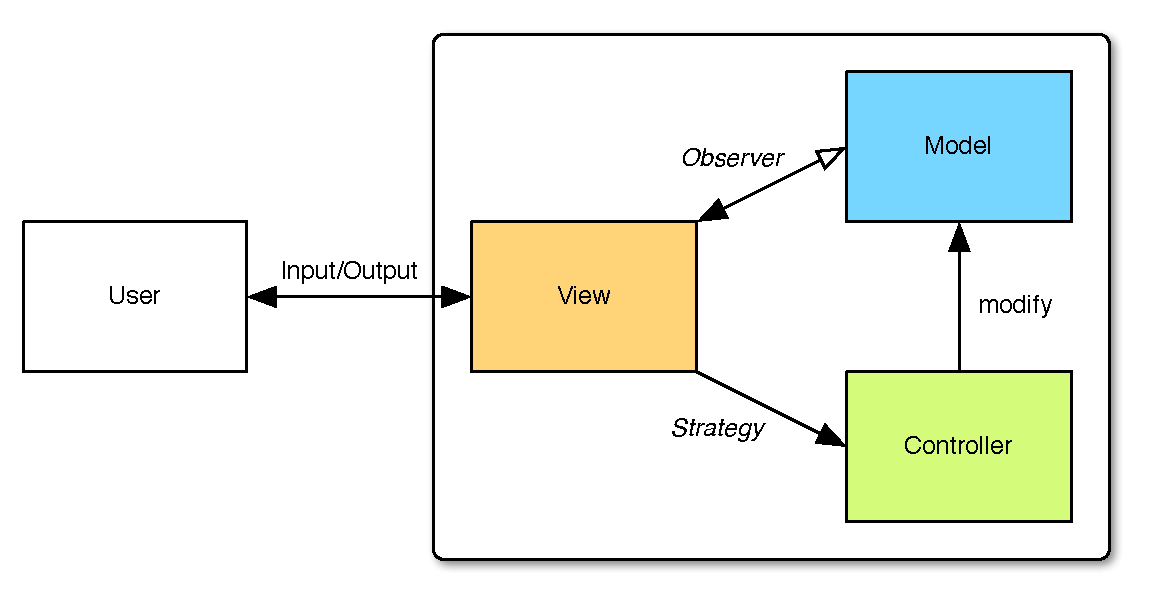
\includegraphics[width=12cm]{images/mvc.pdf}
	\caption{Structure of \acl{mvc}}
	\label{fig:mvc}
\end{figure}



\subsubsection{Model and View}
\label{sec:modelview}
According to \citeasnoun[p. 4]{gof}, ``MVC decouples views and models by establishing a subscribe/notify protocol between them.'' In other words, the View ``subscribes'' to the Model, and the Model then notifies the View whenever the Model's data change. Eventually, the View can update itself to reflect those changes. The \emph{subscribe/notify} solution described by the \emph{Observer} pattern in \citeasnoun[pp. 293--303]{gof} is also called ``Publish--Subscribe'' and allows multiple Views to observe a single Model (see Figure~\ref{fig:modelview}).

\begin{figure}[H]
	\centering
	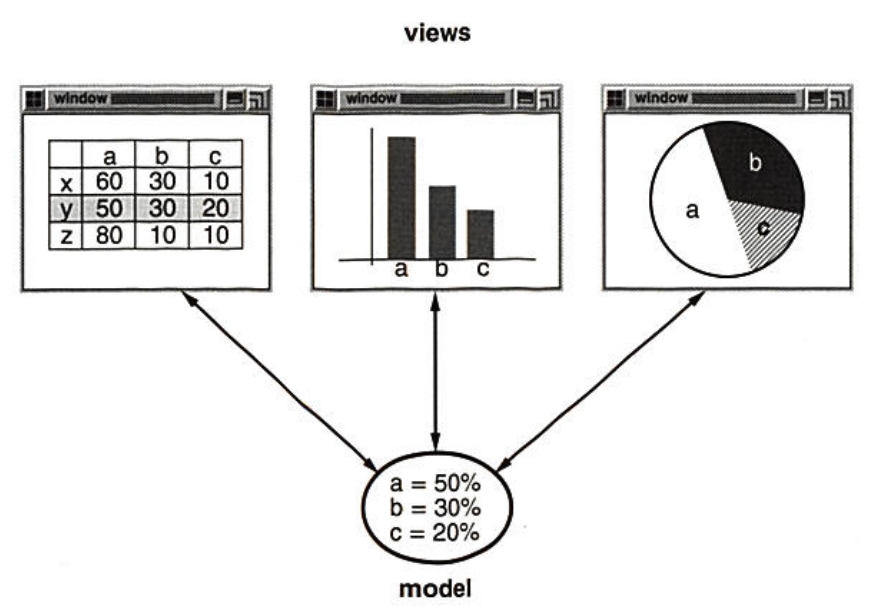
\includegraphics[width=12cm]{images/modelviewhd.png}
	\caption{Multiple Views connected to a single Model}
	\captionsetup{font={footnotesize,bf,it}}
	\caption*{Source: \citeasnoun[p. 5]{gof}}
	\label{fig:modelview}
\end{figure}

According to \citeasnoun[p. 108]{osmani}, the ``observer nature of this relationship is what facilitates multiple views being attached to the same model.'' This means that Model and View are completely decoupled. The Model does not know about the View, it only notifies all its subscribers when it changes. A subscriber can be any arbitrary object, which only needs to implement a special function to receive the notification (in Java, this is typically realized using an \emph{interface}). Thus, a subscriber does not even have to be a View, which means that the Model is completely isolated from the \ac{ui} part of the application (if there is any).

\subsubsection{View and Controller}
The relationship between View and Controller is defined by a Strategy pattern, or in other words: the View uses the Controller as a Strategy object. A Strategy object is an object representing an algorithm. If an interaction is triggered on the View, for example a key press, mouse movement or mouse click, the View recognizes it and invokes the Controller. The Controller then decides on how to react to the according event.

A good example is \emph{scrolling} in a scrollable list. This list (the View) is constrained in its height, so it can only display a part of the list items. List items are stored in the Model. As soon as the user initiates scrolling, for example by moving the mouse wheel or moving the scoll bar, the View calls the Controller. The Controller recognizes the event as scrolling and calls back the View to update itself. Depending on how far the user scrolled, other list items are shown in the list. This course of events is also illustrated in Figure~\ref{fig:seqmvc}.

On his website, \citename{reenskaugweb} describes the pair of View and Controller as the \emph{Tool} (see Figure~\ref{fig:tool}). But, as the Gang of Four writes in \booktitle{Design Patterns: Elements of Reusable Object-Oriented Software}, it is important to keep this coupling loose. This allows a software developer to easily replace a View's Controller, even at runtime, to change its interactive behaviour. The example from \citeasnoun[p. 6]{gof} proposes that, to disable interaction on a View, one could assign to it a Controller that ignores any interaction.
\begin{figure}[H]
	\centering
	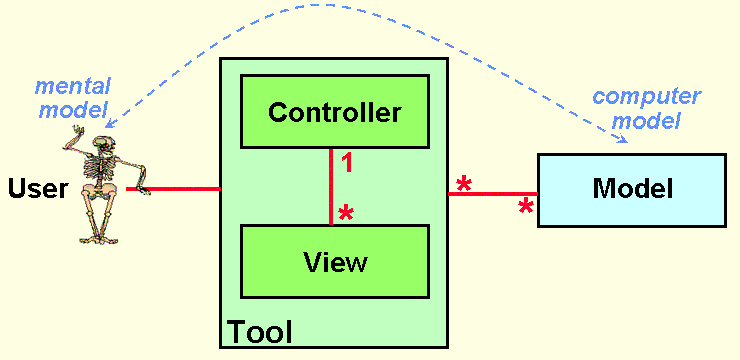
\includegraphics[width=12cm]{images/MVC-2006.png}
	\caption{The Tool contains Controller and View(s)}
	\captionsetup{font={footnotesize,bf,it}}
	\caption*{Source: \citeasnoun{reenskaugweb}}
	\label{fig:tool}
\end{figure}

\subsubsection{Controller and Model}
As described above, one task of the Controller is to react to the user's input. When the user's interaction is targeted at manipulating the domain data, for example by changing the value of a table cell, the Controller's task is to update the Model accordingly.

As mentioned by \citeasnoun[pp. 105, 108]{osmani} and \citeasnoun{reenskaug79b}, the Controller updates the View after the Model changes, but this is not necessary in implementations where the View observes the Model, as is stated in \citeasnoun{fowlergui}: ``When the model changes, the views react.'' The sequence diagram of \emph{Figure 6: Changing the actual value for MVC.} by \citeasnoun{fowlergui} emphasizes that (see Appendix). Subsequently, Addy Osmani clarified that it is ``absolutely correct that the Observer relationship should be responsible for updating the View. The Controller should in no way be changing the View directly.''\footnote{Personal conversation with the author, 07/23/2012}

%The relationship of Controller and Model is unidirectional: the Model does not know about the Controller. In some implementations, the Model might know a Controller via the Observer relationship of View and Model, but as a Controller can also change Models that are not directly associated with its respective View, this is not alway the case.

As it can be seen, the role of the Controller is subject to very different interpretations.

\subsubsection{Flow of Control}
\label{sec:flowofcontrol}
The View and Controller are defined as two very separate objects, the View being responsible for presentation (output), the Controller being responsible for user action (input). It is a matter of definition if a user interaction is performed \emph{on the Controller}, or if it is performed \emph{on the View} and the View then uses the Controller to react to it (\emph{Strategy} pattern). The first variant is illustrated by \citeasnoun{fowlergui} in the sequence diagram of \emph{Figure 6: Changing the actual value for MVC} (see Appendix) as well as by \citeasnoun{steele}. Some sources, however, assume the latter case (the \emph{Strategy} pattern), as it is described in \citeasnoun[p. 6]{gof}. In this thesis, both variants are taken into account, depending on which one makes more sense in a given situation.
\begin{figure}[H]
	\centering
	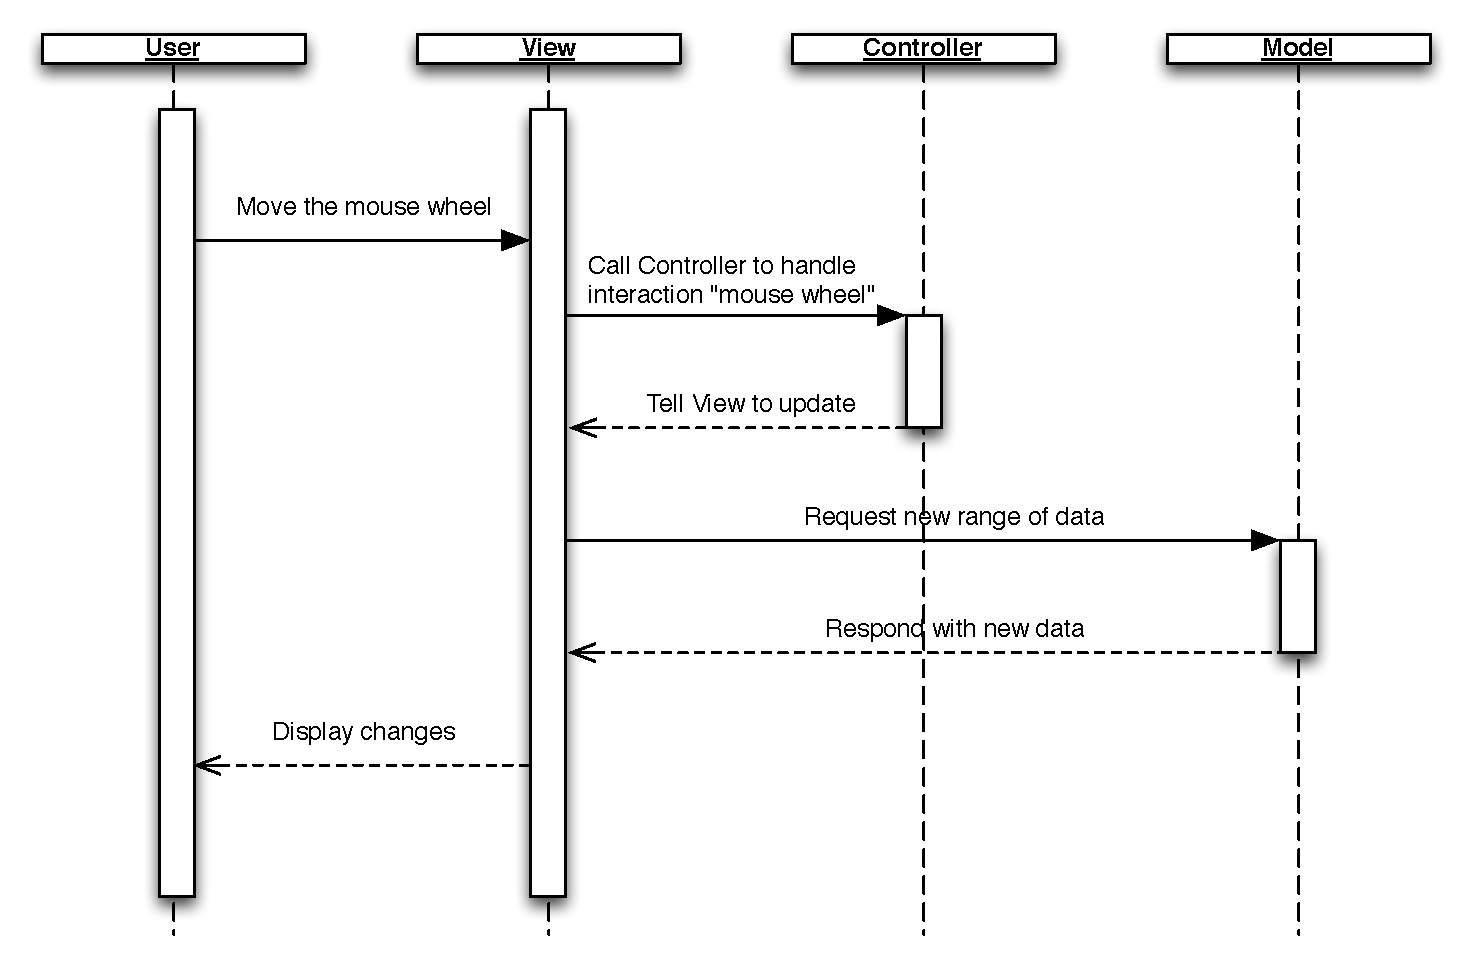
\includegraphics[width=16cm]{images/seqmvc.pdf}
	\caption{Sequence diagram of a User Interaction with \acl{mvc}}
	\label{fig:seqmvc}
\end{figure}
The sequence diagram in Figure~\ref{fig:seqmvc} illustrates the user scrolling over a list of items.

\section{Pattern Variations}
The following section describes variations of MVC that can be found in modern software architecture, especially in web applications and the according frameworks. Those variations are an answer to the different interpretations of \acl{mvc}, primarily regarding the responsibilities of the components. \gls{mvc} and its variations are often called the \emph{MV* family} of patterns \cite{osmani}.

\subsection{Model--View--Presenter}
The first variation of \ac{mvc} to be discussed is \ac{mvp}. It was created in the early 1990s to improve presentation logic for the \gls{Taligent} operating system and has been adapted in a slightly modified form for the use in web applications by the \emph{Backbone.js} framework\footnote{See \url{http://backbonejs.org/}}.

The Model in \ac{mvp} behaves similar to the one of \ac{mvc}: it contains and handles domain data. The difference to \ac{mvc} is in the View and the \emph{Presenter} which replaces the Controller.

The \ac{mvp} View is called a \emph{Passive View}, because it contains as few logic as possible (thus being ``dumb''), as described by \citeasnoun{fowlerpv}.

The Presenter, however, has additional responsibilities compared to the Controller. In Smalltalk-80 \ac{mvc}, the View gets the data to display directly from the Model. In \ac{mvp}, the Presenter separates this connection, acting as a mediator between the View and the Model \cite[p. 109]{osmani}. It decouples Model and View completely by breaking up the Observer connection. The original Controller tasks of manipulating the Model and processing user input are in the responsibility of the Presenter, too.

There are two exceptional advantages in combining the Presenter as a mediator with the Passive View, according to \citeasnoun{osmani} and \citeasnoun{fowlerpv}:
\begin{itemize}
	\item It allows developers to rapidly prototype user interfaces. Most of the presentation and business logic (which is not relevant in the context of prototyping) is in the Presenter, whereas the View is the component being prototyped.
	\item The thin presentation layer embodied by the Passive View makes automated testing possible, which in other cases is hard to do with a user interface.
\end{itemize}

Due to the Passive View, View and Presenter are completely decoupled in MVP. There is no data-binding of the View to the Presenter. This means, it is up to the Presenter to decide how to display data in the View, whereas in other implementations (MVC, MVVM) the View contains the presentation logic.

\begin{figure}[H]
	\centering
	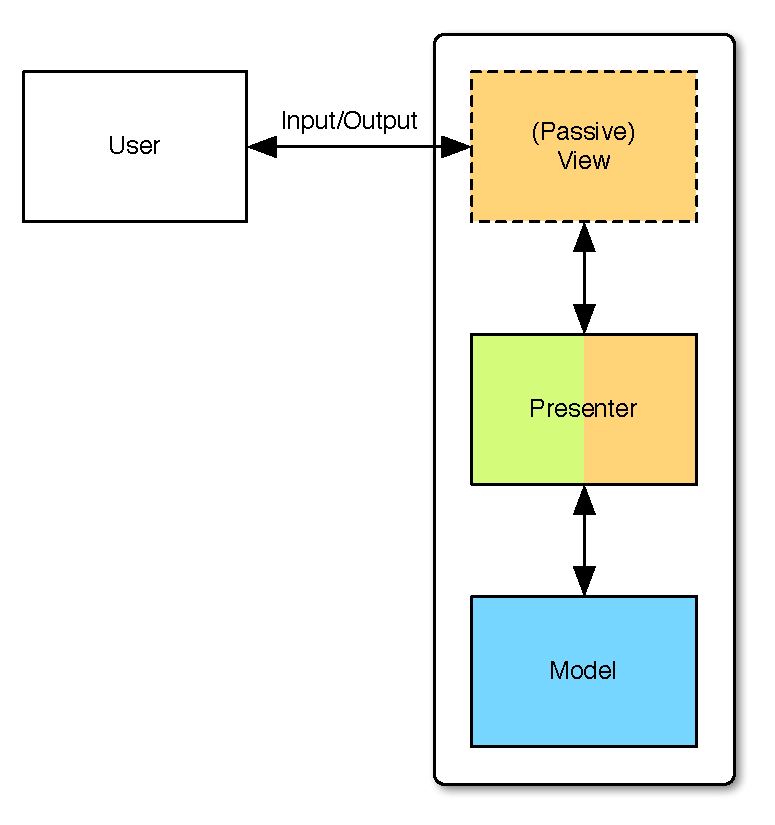
\includegraphics[width=8cm]{images/mvp.pdf}
	\caption{Structure of \acl{mvp}}
	\label{fig:mvp}
\end{figure}

\subsection{Model--View--ViewModel}
A second variation of MVC widely used in web applications is \ac{mvvm}. It was first introduced with Microsoft Silverlight\footnote{Silverlight is a browser extension to include rich media, similar to Adobe Flash.} in 2007. \citeasnoun{poeaa} describes a similar pattern, called ``Presentation Model''. MVVM is based on MVC and MVP and includes concepts of both.

Just as in MVC and MVP, the Model contains domain data and the according CRUD functinality.

In opposition to MVP, the MVVM View is not passive. It contains presentation logic and decides if and when to update itself. In MVP, this task is done by the Presenter. The Presenter ``pushes'' changes of the Model to the View, whereas the ViewModel only ``notifies'' the View of those changes; it is up to the View to request the changed data and format them to its purpose.

The term ``ViewModel'' is caused by this component acting like a View-specific Model. Just like the Presenter in MVP does, it decouples the View from the Model and acts as a mediator between them. The difference to a Presenter is, that the ViewModel handles data modelling rather than presentation. It listens for changes in both the Model and the View and synchronizes them, doing only basic data conversions\footnote{For example, the conversion from a UNIX timestamp (``1342177280'') to a localized timestamp (``July 13, 2012 11:01:20'').}.

ViewModel and View are connected through bidirectional data bindings, which act as the single interface between these two components. In its relationship to the View, the ViewModel can be compared to the MVC Model, which also notifies the View of changes, but does not change the View directly.

From a high level point of view, the structures of MVVM and MVP are the same. The differences are in the responsibilities and the coupling of the components; Figure~\ref{fig:mvp} and Figure~\ref{fig:mvvm} illustrate this using colors representing the responsibilities of the MVC components, which are differently distributed in MVP and MVVM.

\begin{figure}[H]
	\centering
	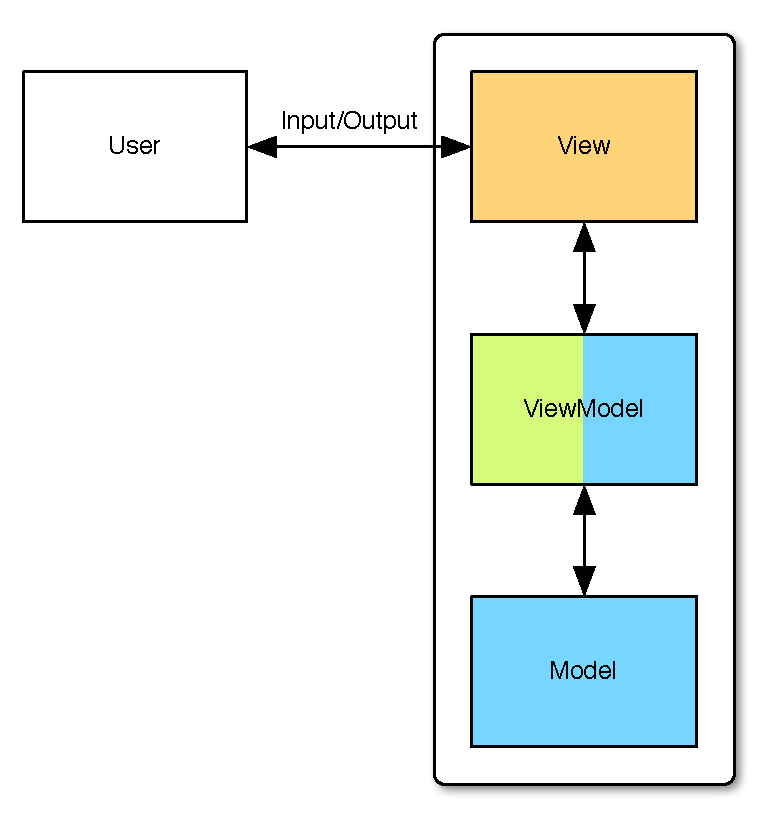
\includegraphics[width=8cm]{images/mvvm.pdf}
	\caption{Structure of \acl{mvvm}}
	\label{fig:mvvm}
\end{figure}


\subsection{Comparison of MVC, MVP and MVVM}
The following example illustrates the differences between MVC, MVVM and MVP: A part of an application displays a list of tasks. In the Model, they are organized as an array of task objects, each of which has different attributes, such as the task name, the due date and the state (``done'' or ``not done''). There are a hundred tasks, but the UI has to display only the first ten tasks.

In MVC, the View fetches the data it needs (the first ten items) directly from the Model. As the View already is a list presentation, it only needs to add the tasks as list items. The Controller is not involved in this process.

In MVP, the Presenter fetches the items it needs (the first ten) from the Model. It then formats them as a list with every list item having a check box next to it. This list gets forwarded to the View and is displayed there.

In MVVM, the View tells the ViewModel that it needs the first ten task items. The ViewModel then fetches those items from the Model and send them to the View. The View formats them as a list.

Basically, all three patterns fulfill the same tasks. As mentioned before, the difference is in the responsibilities of the various components.

The MVVM View contains more presentation logic than the MVP one, its structure is given and it prepares the data for presentation itself (except for logical conversions). In MVP, this is the Presenter's task, while the View keeps passive.

Both MVP and MVVM decouple the Model from the View, in opposition to MVC. The direct access from the View to the whole Model in MVC is considered bad by \citeasnoun[p. 123]{osmani}, as it can ``have security and performance costs''. In other words, access to the Model is neither controlled nor cached. The missing ability to cache data in MVC may be a downside compared to MVP and MVVM, but on the other hand, there is less processing of data between View and Model. When data conversions in Presenter or ViewModel are complex, this can be an advantage for MVC.

It is a matter of preference and use case to choose the architectural pattern that suits an application best. In the following chapters, especially in Chapter~\ref{chap:webmvc}, MVC is assumed to be the pattern used, but the components marked as Model, View and Controller do not have to be distinct objects --- it is more important to understand that they fulfill the tasks and have the responsibilities of the respective MVC components, as described earlier in this chapter.
\chapter{Web Application Architecture}
\label{chap:webapparch}
This chapter describes the architecture of web applications. After an introduction to different web and web-related technologies and their roles, the differences between \emph{thin client} and \emph{rich client} web applications are discussed.
\section{Supporting Technologies}
The following section gives an overview of different technologies that are used in web applications (and other browser-based applications) nowadays. This list does not claim to be complete, but it covers those technologies important for the discussion.
\subsection{Server Side}
\begin{description}
	\item[\gls{http}] is the application layer network protocol of the web. \gls{http} is a textual, stateless protocol using \acs{tcp}. In a web environment, a web server --- such as Apache, Lighttpd, or Microsoft \gls{iis} --- acts as the \gls{http} server, whereas a web browser usually acts as the \gls{http} client. Not only web pages are transferred using \gls{http}, but also resources like \ac{css}, scripts (e.g. JavaScript files), \gls{xml} data and images. \gls{http} is an open standard developed by the \gls{ietf} and the \gls{w3c}.
	\item[HTML Preprocessors] are compilers or interpreters that generate \gls{html}. Some programming languages are especially built for this purpose, but in general, every programming language and compiler can be used to generate \gls{html}. Some of these preprocessors, such as \acs{php}, Perl and Python, are invoked through the \gls{cgi} of web servers. Others are used with application servers instead, for example \gls{asp}, ASP.NET, and \gls{jsp}. In the area of enterprise applications, \gls{jsp} has become the established standard.

	HTML preprocessors allow the dynamic generation of HTML, XML and other resources through the use of --- mostly imperative --- programming languages. The power of functions, variables and \glspl{api} can be used, for example to query a database and process the received data. This allows to overcome the statelessness of \gls{http}.
	\item[Application Servers] provide commonly used \glspl{api} and frameworks to applications, enabling them to use features such as security, load balancing, database connections or \gls{mvc}. Application servers are often used for enterprise applications, as they can shorten development time significantly. The most popular examples, such as Red Hat JBoss, Apache Tomcat, or IBM \gls{was}, can deploy Java and \acs{jee} applications, but there also are application servers for other programming languages, such as Zope for Python and Zend Server for \gls{php}. Usually, application servers include an \gls{http} server for the communication with web browsers, but this task can also be handled by a third-party web server.

	\gls{jee} application servers provide a \gls{jre} and consist of multiple components, including the following:
	\begin{itemize}
		\item The \emph{Servlet container}, also called \emph{web container}, manages \emph{Servlets} and maps them to a \gls{url}. A Servlet is a Java class that serves a client request with a special response, most often via \gls{http}. In other words, the Servlet container is the application server's interface to the web browser.
		\item The \emph{\gls{jsp} container} translates \gls{jsp} files into Servlets at runtime. \gls{jsp} features a templating system for \gls{html} that allows developers to embed Java code into \gls{html}.
		\item The \emph{\acs{ejb} container} manages \emph{\gls{ejb}}, which are components that encapsulate business logic in \gls{jee} applications. EJBs run back-end code and execute tasks like database access, messaging and web service invocation.
	\end{itemize}
	There are more components in the \gls{jee} specification, but they are not relevant in this context.
\end{description}
\subsection{Client Side}
\begin{description}
	\item[\gls{html}] is a markup language to represent hypertext\footnote{Hypertext resembles the thinking of human beings, in opposition to sequential text. Hypertext contains semantics and links to other texts, and is therefore non-linear.}. It was created by Tim Berners-Lee, who also developed the first web browser. \gls{html} consists of elements described by \emph{tags} which are enclosed by angle brackets. Tags often give semantics to elements, such as headings, emphasized text, lists or tables. Web browsers build a \gls{dom} out of \gls{html} code and display it as a web page.
	\item[CSS3] \gls{css} is a W3C standardized language to describe the look (``style'') of markup elements. It can be used, for example, to format and style an HTML document. The third generation of CSS adds more possibilities for designing user interfaces for web applications. In the past, visual enhancements such as shadows, gradients or non-standard fonts had to be provided by image files, and animations had to be programmed using JavaScript. CSS3 is capable of doing most of that while using less bandwidth and ensuring standards conformity, thus enhancing the performance and usability of websites. Some modern browsers even use hardware acceleration for CSS3 animations and effects. CSS3 makes complex user interface design possible on the web while separating the presentation from the content.

	In combination with CSS preprocessors\footnote{CSS preprocessors allow the creation of CSS from more versatile and powerful languages that are especially designed for this reason. Those languages, such as SASS, LESS, or Stylus, provide advanced features known from imperative languages, like variables and functions.}, such as SASS, LESS, or Stylus, development time can be reduced significantly.
	\item[JavaScript] is, according to \citeasnoun[p. 1]{flanagan}, ``the programming language of the web.'' It is a weakly~typed multi-paradigm language (functional and object-oriented), created 1995 by Brendan Eich at Netscape \cite{eich}. It is standardized as \emph{ECMAScript}, the latest version being ECMAScript 5.

	Most modern web browsers, such as Mozilla Firefox, Google Chrome, Opera or Microsoft Internet Explorer 9, provide a JavaScript engine and thus are able to execute JavaScript. Although they are not part of the language itself, \glspl{api} are provided by browsers to manipulate the \gls{dom} and use other browser functions, such as the browsing history. An event--callback system offered by the browser \gls{api} allows developers to build interactive web sites, in opposition to static ones based solely on \gls{html}. Different libraries and frameworks, such as Dojo, jQuery or Prototype, exist to simplify web application development with JavaScript.

	There are also server-side implementations --- for example \emph{Node.js}, which is based on Google's V8 JavaScript engine --- but they are not relevant in this context.
	\item[\gls{ajax}] is not a technology, but a method to allow dynamic loading of content, even after the actual web page has completely loaded. Using \pathname{XmlHttpRequest}, an object provided by the browser, HTTP requests can be sent from within JavaScript. The response, once returned, can then be processed in the background. The request is asynchronous, which means that the web page is not blocked while waiting for the response; it continues reacting to user input. This is especially important if the web page should feel like a desktop application.

	The method is called \acl{ajax}, because the response format often is \gls{xml}. However, this does not need to be the case. The response can be of any kind, for example an image, \gls{html} or \gls{json} data. \gls{json} is a subset of the JavaScript language, which means it can directly be included into the running script. Literals, objects and arrays can all be serialized as \gls{json}. In comparison to \gls{xml}, \gls{json} has a small footprint and a more flexible structure. The latter can, but not must, be a disadvantage.

	\item[HTML5] is the latest version of \gls{html}, which defines new elements and additional JavaScript \glspl{api}. Some of these \glspl{api} can be an advantage for MVC-based web applications, including:
	\begin{itemize}
		\item The \emph{Web Workers \gls{api}} relaxes the single-threaded client-side JavaScript model to support multiple threads, called ``workers''. Workers are to classic operation system threads; they do not share memory (thus, they lack access to the \gls{dom}) and can only communicate with the main thread through asynchronous messaging~\cite[pp. 680--687]{flanagan}. Nevertheless, Workers make it possible to execute multiple tasks in parallel without blocking each other or the user.

		\item Using the \emph{WebSocket \gls{api}}, long-living \acs{tcp} connections can be established. When using \gls{ajax} to communicate over the network, \gls{http} is always involved, which is a stateless (session--less) protocol. Opposed to that, WebSocket connections can be persistent and allow data to be sent and received as long as the socket is open. As WebSockets bring their own protocol on top of the \gls{tcp}, the server being queried also needs to support that protocol. There exist several libraries to add support to web servers, for example an Apache and a Node.js module \cite[pp. 712--716]{flanagan}.

		When used together with Web Workers, WebSockets can provide a web application with threaded network functionality. This is also relevant for MVC applications with real-time Model synchronization, as WebSockets can be used to notify the client of an updated server-side Model. This is further discussed in Section~\ref{sec:realtime}.

		\item The client-side \emph{Storage \glspl{api}} allow an application to store structured data within the web browser's sandbox. Before, only \gls{http} Cookies could be employed for client-side data storage, but Cookies are limited in size and they allow only textual data to be included. One of the new \glspl{api} is \emph{IndexedDB}, an object database that is currently supported in Firefox and Chrome, whereas the relational \emph{Web SQL} database is implemented in Chrome, Safari and Opera. The \emph{Filesystem API} allows web applications to create, delete and manipulate files and directory structures in a sandboxed environment. All web applications with the same origin (host, port, and protocol) share one filesystem --- this is a concept borrowed from HTTP cookies to avoid unauthorized access to data from the wrong web application.~\cite[pp. 700--712]{flanagan}

		These \glspl{api} can be used to allow advanced storage of data, breaking with the 4KiB limitation of \ac{http} cookies. They can be used for caching and client-side persistent storage. It is even possible to write offline applications using these APIs.
	\end{itemize}
\end{description}

\section{Client--Server Architecture on the Web}
\label{sec:clientserver}
This section describes the general architecture of 2--tier web applications, and then discusses the terms ``Thin Client'' and ``Rich Client'' in this context.

The first tier, also called ``client'', is the end user's web browser. The second tier, the ``server'', is a web server on the internet or inside a local network, for example a company's intranet. The key technology for this architecture is the \acs{http} protocol that has to be understood by both client and server. Thus, the web browser acts as an \acs{http} client and the web server acts as an \acs{http} server.

The common interaction between the user, a client and server using HTTP is further described by the following sequence diagram in Figure~\ref{fig:http}

\begin{figure}[H]
	\centering
	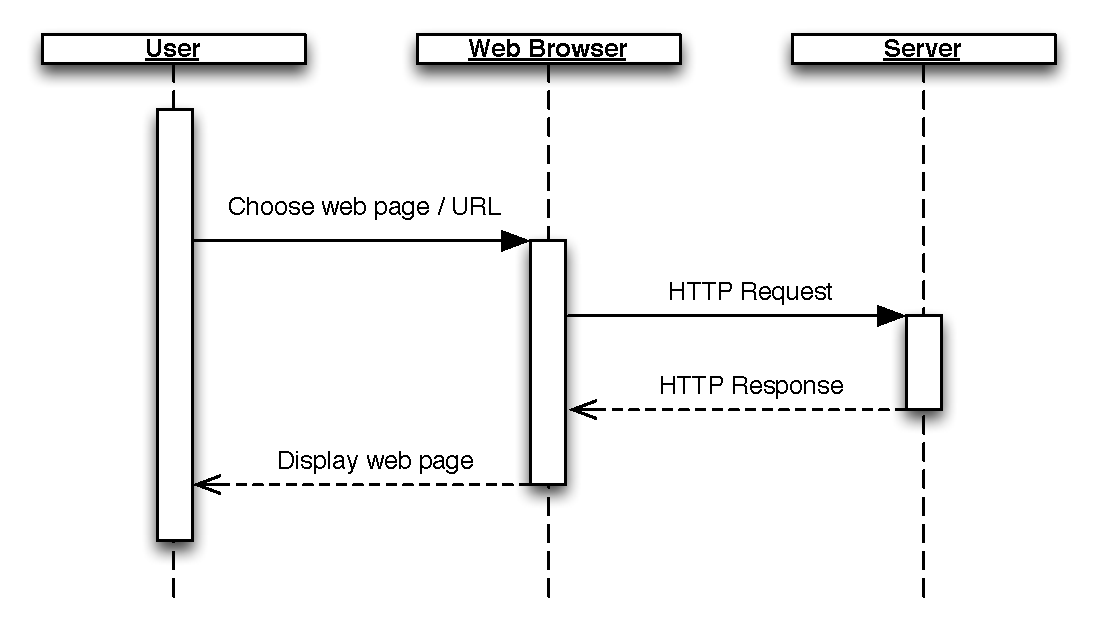
\includegraphics[width=16cm]{images/http.pdf}
	\caption{Sequence diagram of a User--Client--Server interaction}
	\label{fig:http}
\end{figure}

The actual HTTP request is illustrated in Listing~\ref{lst:http}. Such requests have to be made for every resource loaded from the server, such as \gls{html}, JavaScript, images and stylesheets (\gls{css}). As every request includes protocol overhead, the number of requests to be made is an important factor to the performance of a web application. This is further discussed in Section~\ref{sec:datavolume} and Section~\ref{sec:mvcwebarch}.
\begin{listing}[H]
\begin{minted}[linenos=true]{http}
GET /index.html HTTP/1.1
Host: www.example.com

HTTP/1.1 200 OK
Date: Mon, 23 May 2005 22:38:34 GMT
Server: Apache/1.3.3.7 (Unix) (Red-Hat/Linux)
Last-Modified: Wed, 08 Jan 2003 23:11:55 GMT
Content-Length: 438
Content-Type: text/html; charset=UTF-8

... Response body ...
\end{minted}
\caption{HTTP conversation}
\label{lst:http}
\footnotesize{\textbf{\textit{Source: \citeasnoun{wiki:http}}, modified by the author}}
\end{listing}
%Etag: "3f80f-1b6-3e1cb03b"
%Accept-Ranges:  none
%Connection: close

\subsection{Terminology}
\label{sec:terminology}
In computer technology, the terms ``Thin Client'' and ``Rich Client'' (also: ``Thick Client'' or ``Fat Client'') have multiple meanings, so it is necessary to define their meanings in this context.

These two terms often describe computer hardware. A Thin Client in the hardware context is a computer that heavily depends on another computer (e.g. a server) to fulfill its computational role, whereas a Rich Client not only handles input and output (I/O), but also processes data.

This concept of dependance also applies to web applications. In that context, the Thin and Rich Client are not computer hardware, but rather represent the client side of a web application (thus, they are software running \emph{inside a browser}).

The term ``Rich Internet Application'' also is sometimes used for web applications with a Rich Client, but it more often refers to applications powered by browser plug-ins, such as Adobe Flash or Adobe Flex.

The following two definitions are kept generic and reflect the fact that there are different variations in the range from a Thin to a Rich Client. Four of those variations are further discussed in Section~\ref{sec:mvcwebarch} with respect to an \ac{mvc} architecture. Both definitions are examined from both a user and technology perspective.

\subsection{Thin Client}
\label{sec:thinclient}
We can also refer to the Thin Client as the classical way of writing web applications. From a user perspective, a Thin Client feels like a usual web site. Every time the user switches the perspective or navigates to a different part of the web site, the \gls{url} changes and a whole page is loaded from the server. This is, for example, the fact with \url{http://www.craigslist.com/}\footnote{Craigslist is a classifieds platform extremely popular in the United States.}. If you switch between categories at the Craigslist web site, the whole page gets loaded and rendered again.

This is due to the fact that in many Thin Clients, every page of a web site either has its own \gls{html} file, or gets preprocessed on the server (using \gls{php}, \gls{asp}, \gls{jsp} or any other preprocessor) depending on defined parameters\footnote{These parameters may, for instance, be GET or POST parameters of the respective \gls{http} request \cite**{http}.}. From a technology perspective, a page is --- when requested --- constructed on the server side and sent over to the client side. There are no subsequent data loaded (except for resources already specified in the original page). The page is dynamically generated, but the web application is not interactive.

From the perspective of software architecture, a Thin Client is static and ``dumb''. Most of the business logic and data --- and thus, most of the \ac{mvc} structure if this is the used architectural pattern --- is on the server. The content gets prepared on the server, processed with real data and is then sent to the client. However, the client does not know where the data are from and how to retrieve additional or updated data. Also, it is not able to further process the data without communicating with the server. This means that a user can modify data on the client side, but these data must be sent back to the server side to be processed and then the updated page has to be retrieved again.

The sequence diagram (Figure~\ref{fig:seqthinclient}) shows the process of a user requesting a web page and then updating data using a Thin Client / Rich Server with an additional database tier. Business logic, for example input verification, is executed on the server. After updating the data, the whole web page has to be preprocessed on the server, sent to the client and displayed again. The browser and user are inactive during this time.

\begin{figure}[H]
	\centering
	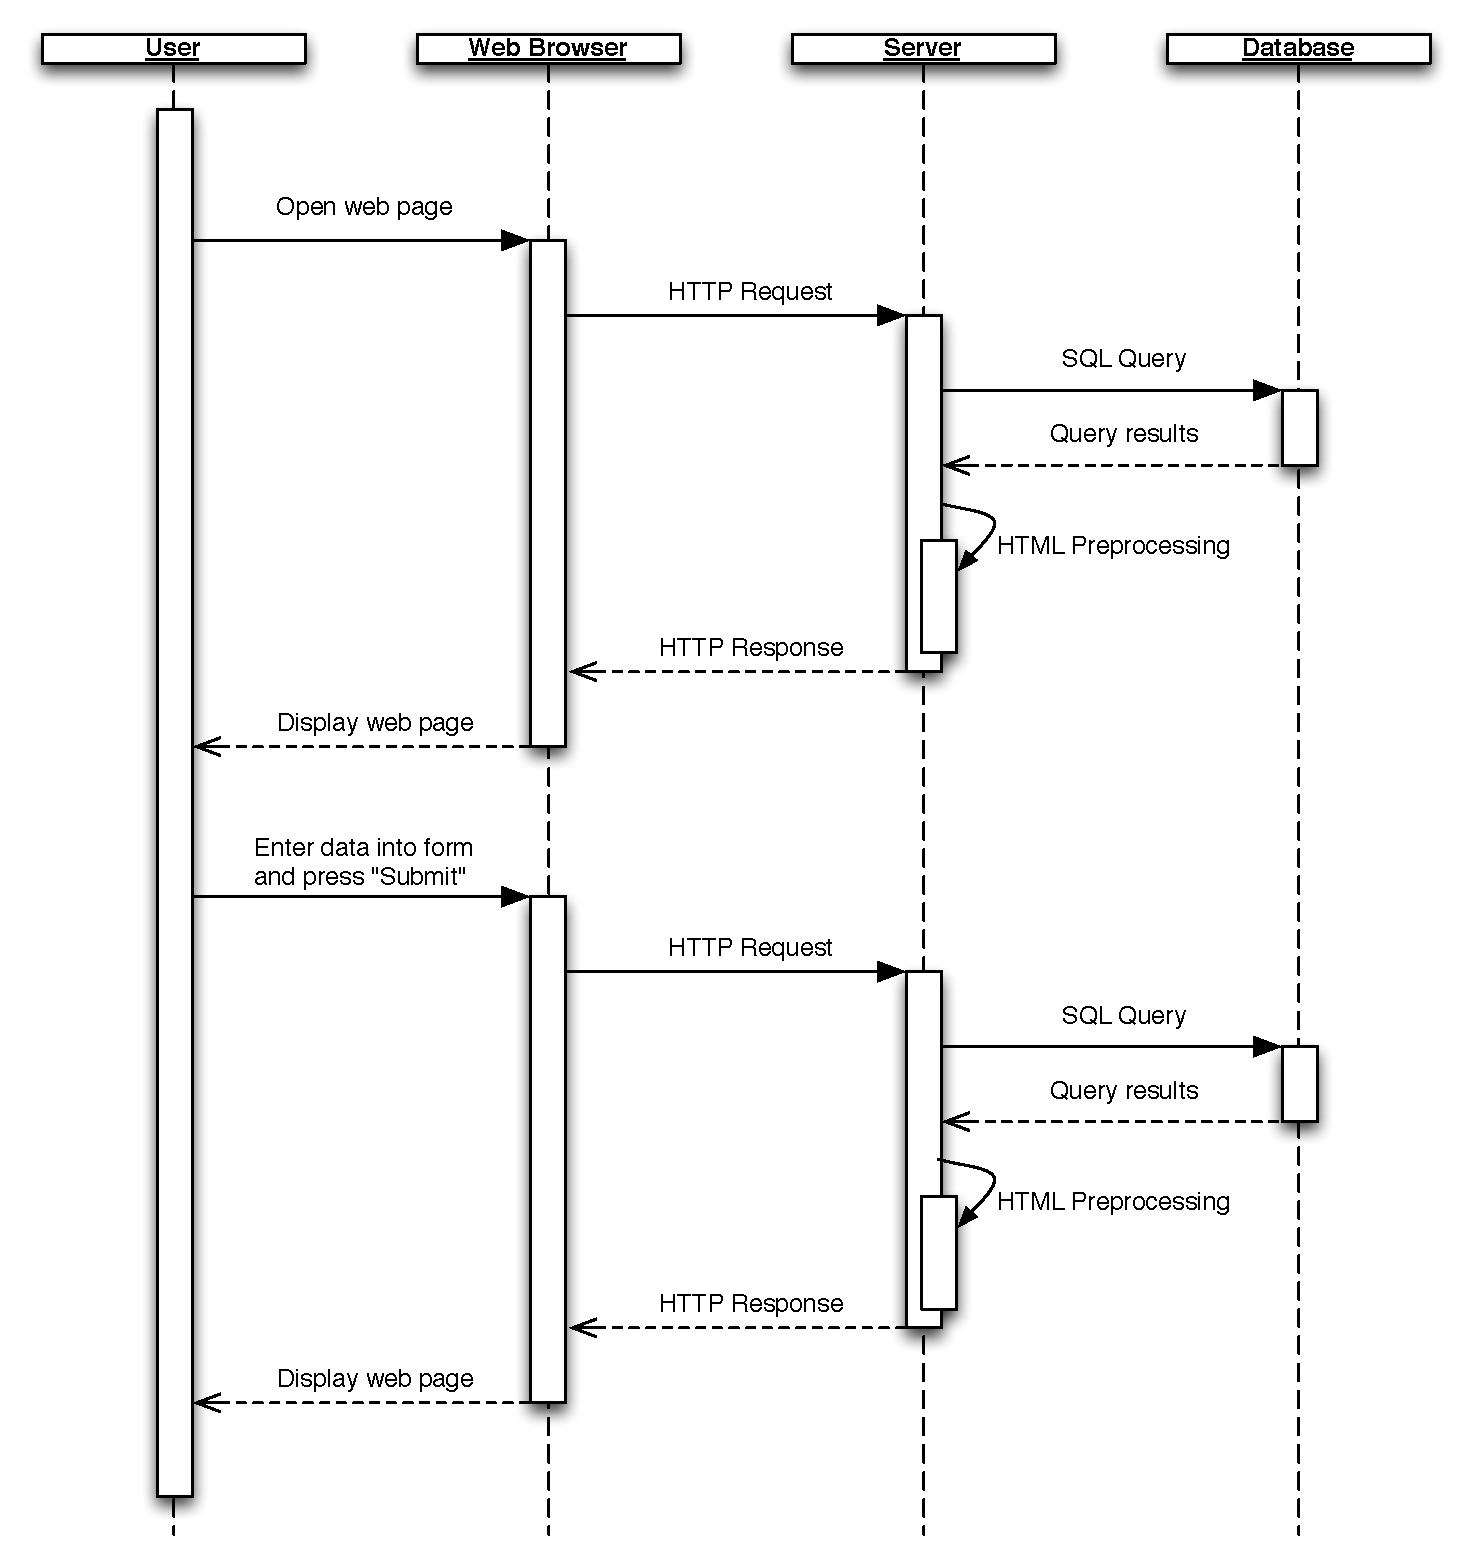
\includegraphics[width=16cm]{images/seqthinclient.pdf}
	\caption{Sequence diagram of a Thin Client user interaction}
	\label{fig:seqthinclient}
\end{figure}

An illustrating example for a Thin Client / Rich Server model are the two variants of \acl{mvc} in \ac{jsp}--based web applications, called \emph{Model 1} and \emph{Model 2}. As described by \citeasnoun[pp. 444--446]{johnson}, Model 1 provides individual \ac{jsp} pages for every section of the web application, mapping those pages to \acp{ejb}. The flow of navigation is directed by links to the different JSPs, which act as both Controller and View. The JavaBeans are the respective Models.

\begin{figure}[H]
	\centering
	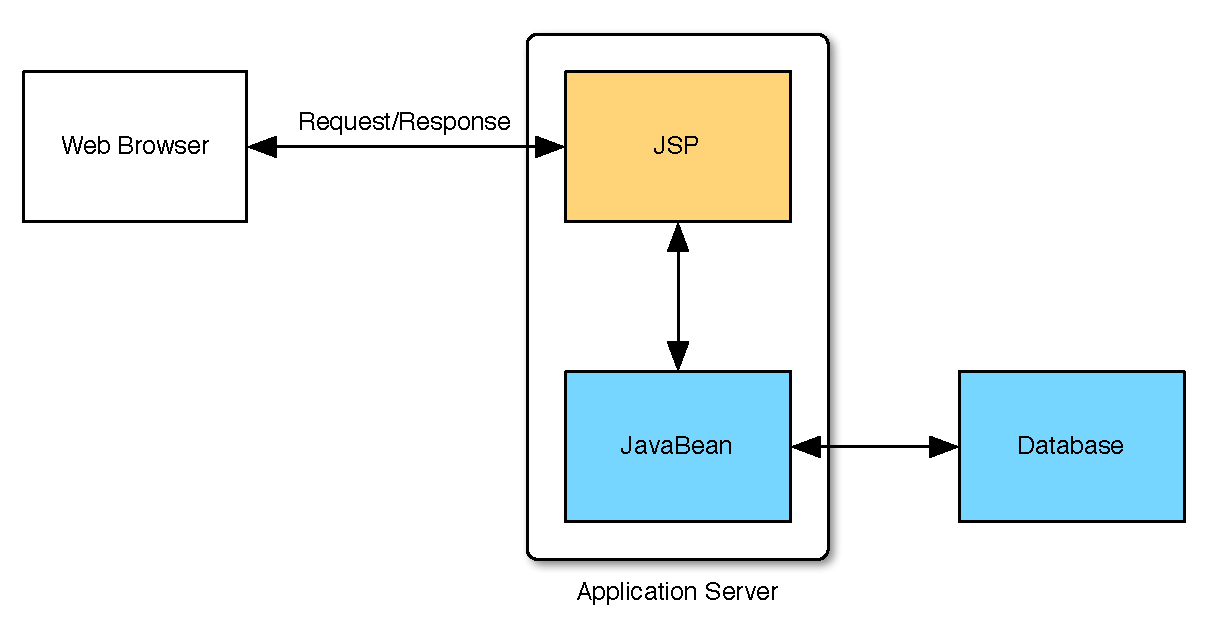
\includegraphics[width=14cm]{images/model1.pdf}
	\caption{JSP Model 1 Architecture}
	\label{fig:model1}
\end{figure}

In Model 2\label{term:model2}, the Controller part is encorporated by one central Servlet acting as an entry point into the application \cite[pp. 446 f.]{johnson}. It handles all browser requests and manages the application state. Depending on the request and the state, it selects a View (\ac{jsp}) to serve back to the browser. Similar to Model 1, the View communicates with the Model (JavaBean), but the JavaBean is modified by the Servlet instead of the \ac{jsp}. Having only one Controller differs from the \mbox{Smalltalk-80} definition of \ac{mvc}, but can be seen in some interpretations as an \emph{application controller}.

\begin{figure}[H]
	\centering
	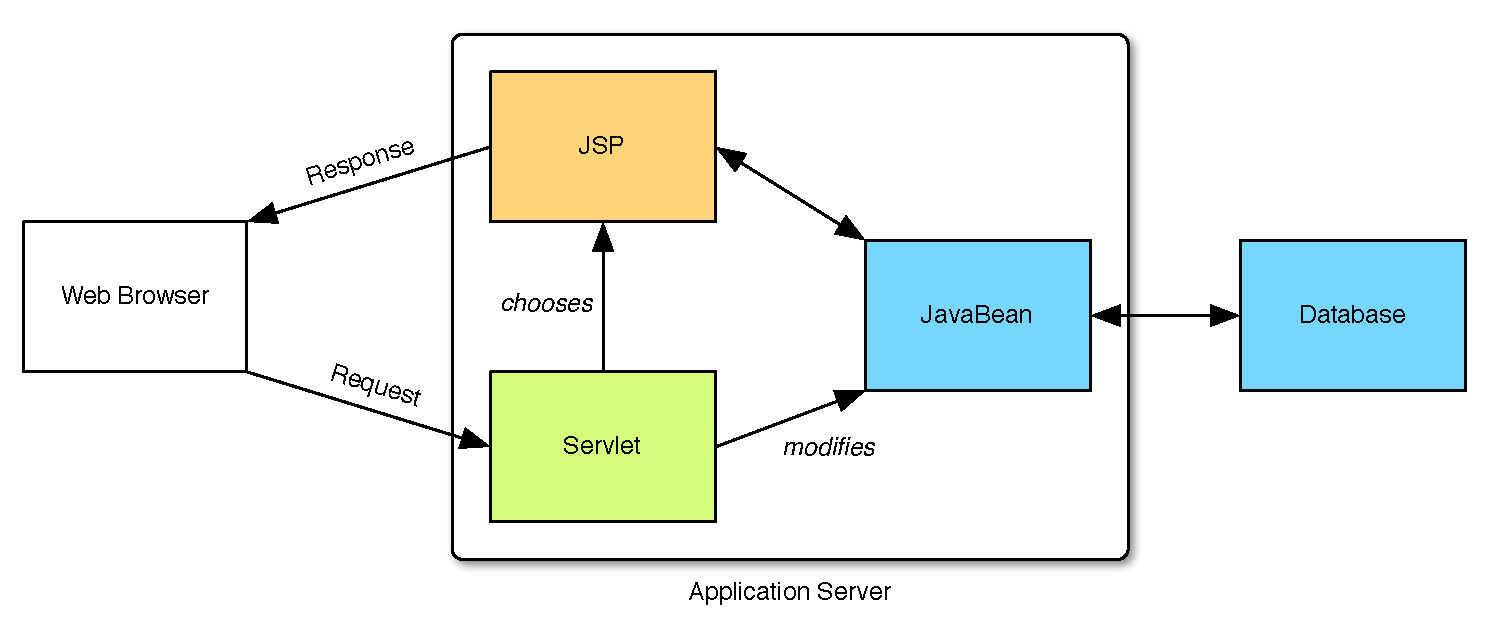
\includegraphics[width=16cm]{images/model2.pdf}
	\caption{JSP Model 2 Architecture}
	\label{fig:model2}
\end{figure}

\subsection{Rich Client}
% Ein Fat Client ist neben der Ein- und Ausgabe auch für die Verarbeitung der Daten zuständig. Lediglich zur Kommunikation und Datenspeicherung werden Dienste eines Servers genutzt. % wikipedia
From the user perspective, the key difference to a Thin Client is that the Rich Client acts \emph{like a desktop application rather than a website}.

From a business logic perspective, a Rich Client web application runs as much application logic as possible on the client side. This means, data transformation (like sorting, filtering, conversion) and referencing happens on the client side, as well as changes to the data (which then are made persistent on the server side). There still are parts that have to be executed on the server, for example security (authentication, authorisation) and the connection to a third tier (such as a database).

From a technology perspective, a Rich Client makes extensive use of JavaScript and the \ac{ajax} technique.
%This does not mean that a Thin Client has to run without JavaScript and asynchronous calls, it just means that a Rich Client leverages the power of JavaScript.
This can, for example, happen through the use of a client-side MVC pattern that has not only the View, but also the Model and the Controller running in the browser. In modern scenarios, another example is the use of Web Sockets that lets the server-side Model notify the web browser when changes happen. The key point is to reduce communication with the server to a minimum.

Figure~\ref{fig:seqrichclient} shows a sequence diagram of a user interaction with a Rich Client / Thin Server. The same activities as in Figure~\ref{fig:seqthinclient} are executed, but due to the asynchronousness of \ac{ajax} calls, the browser and user can still interact during the second request. As indicated, the web page gets only preprocessed once (when first requested). After the form submit, the processing of the returned, updated data happens in the browser, and not on the server as in Figure~\ref{fig:seqthinclient}.

Also, business logic such as input verification is executed on the client-side already (before the form is submitted). However, to ensure data consistency and security, in most implementations the submitted data --- as well as the user's authorization --- is verified on the server again.

In extremely client-sided web applications, such as \ac{ibm} \nexus, there happens no preprocessing on the server at all. On first request, the server only sends one single, nearly empty \ac{html} skeleton file. The client loads all needed functionality (mostly Dojo and \ac{idx}) via \ac{ajax}, building the \ac{gui} solely using JavaScript. There are no more ``pages'' in the sense of web pages; navigation is done using JavaScript. If the user navigates to a different application pane, \nexus\ swaps out the respective \ac{dom} nodes, which gives the feel of a real desktop application. \nexus\ is further discussed in Chapter~\ref{chap:nexus}.

This navigational pattern is described by \citeasnoun[pp. 104 f.]{osmani} with one main characteristic: the state of the application is managed on the client side, using a component that has the role of a ``router''. In Thin Client applications, the state is managed on the server side using sessions\footnote{A \gls{session} identifies interrelated requests using a session ID (usually a unique combination of alphanumeric characters) to provide state on top of the stateless \ac{http} protocol.}.

\begin{figure}[H]
	\centering
	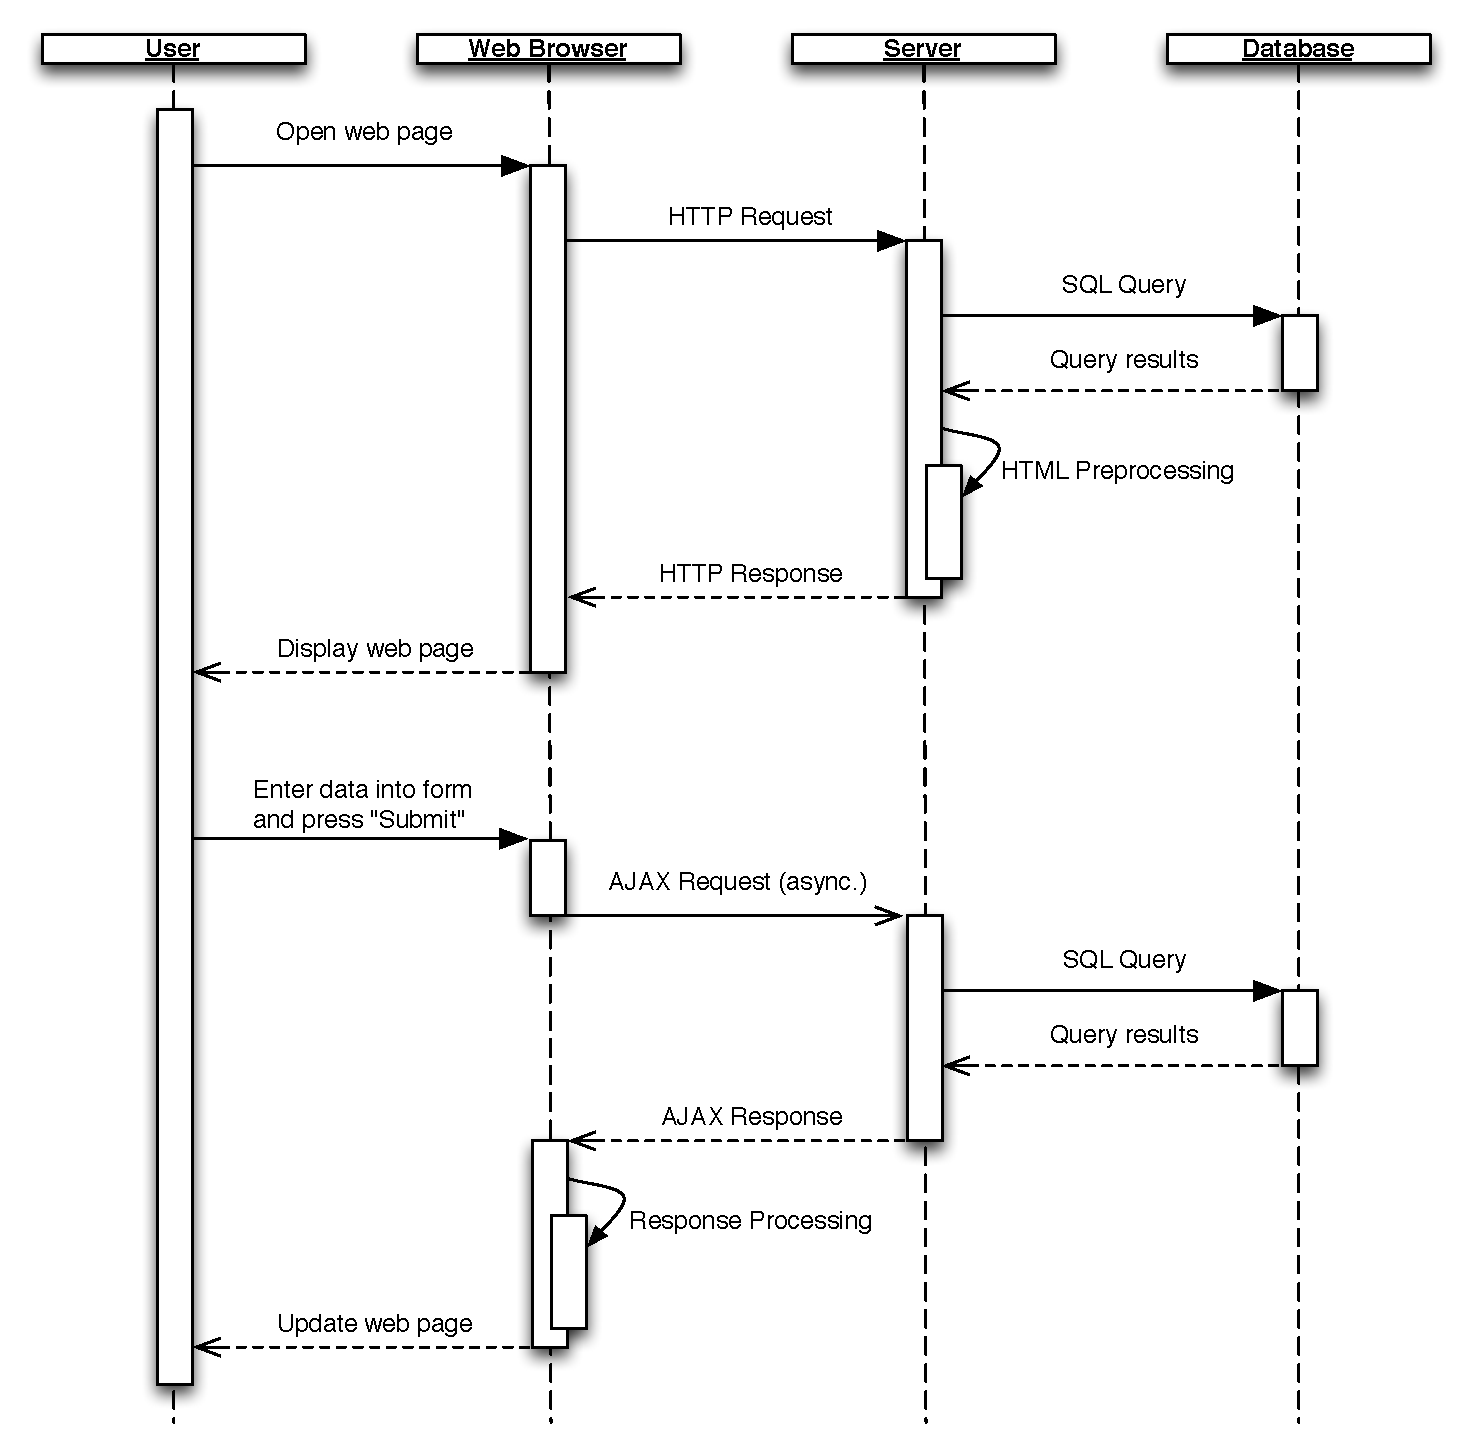
\includegraphics[width=16cm]{images/seqrichclient.pdf}
	\caption{Sequence diagram of a Rich Client user interaction}
	\label{fig:seqrichclient}
\end{figure}

%===============
% Applicability
%===============

\chapter{Applicability of Different MVC Architectures for Web Applications}
\label{chap:webmvc}
In the previous two chapters, the \acl{mvc} pattern as well as technologies and techniques relevant to web application architectures have been presented. The challenges that result from applying MVC to web applications are discussed in this chapter by means of three defined criteria and four different MVC architecture variations.

\section{Evaluation Criteria}
In this section, three criteria --- \emph{data model complexity}, \emph{real-time model synchronization}, and \emph{data volume} --- are defined to help evaluating the applicability of different possibilities to implement \ac{mvc} in web applications. These criteria are accompanied by problems that have to be solved by an appropriate architectural design.

Some of the criteria are quantitative and can thus be evaluated objectively, such as \emph{Data Volume}. Others, such as \emph{Data Model Complexity}, are rather intangible and thus have a high interpretability. Therefore, examples are given to illustrate each criterion.

%=============================================================================
%=============================================================================

\subsection{Data Model Complexity} % gegeben
\label{sec:complexity}
Data model complexity is a criterion that cannot be measured objectively, and is also hard to define. It is an inherent problem for many domains that needs to be solved by an adequate web application architecture.

The complexity of a data model can best be illustrated by means of a relational database. The more the data model is normalized, the more complex it is. Normalization of data means to minimize redundancy and dependency. Normalized data often have cross references --- foreign keys in relational databases, object references in object--oriented programming languages and databases.

For Model--View--Controller based web applications, complex data models lead to a large number of Models and references between different Models. This can have challenges for the software design on the one hand, and for maintaining data consistency on the other hand.

\subsubsection{Examples}
A simple \emph{task application} with the only domain data being ``tasks'' has no high data model complexity. There usually is an additional Model for the users, but this never has to be managed on the client side. Users do not interfere with each other in this application, and they can only access their own tasks. A good example for an application of low data model complexity is \emph{Do It (Tomorrow)}\footnote{See \url{http://tomorrow.do/}}.

A project management application that manages users and roles, teams, projects, tasks and milestones and provides both an end-user as well as an administrator interface, has a high data model complexity.

\acl{icn} also is an illustrative example for web application with a complex data model. There are not only nested and interconnected Models, but also different data sources for the Models. \ac{rest} services can either be directly connected using Dojo, or they are accessed using the service layer of ICN as a proxy. In the latter case, Dojo interfaces with a service that acts as a REST API and redirects every request to the actual REST server after applying advanced business logic --- such as authentication and authorization. This can, for example, be used for \ac{sso}. Other data sources, such as the content repositories FileNet P8 and ContentManager, also have to be included. The fact that Content Navigator supports multiple repositories through \ac{sso} in one single interface leads to an even higher complexity. ICN is described in Chapter~\ref{chap:nexus} in more detail.
% separation of concerns, also in web app <-- ich hab keine ahnung mehr, was ich damit sagen wollte... =/

%=============================================================================
%=============================================================================

\subsection{Real-time Model Synchronization} % nfq
\label{sec:realtime}
In the area of web applications, the term \emph{real--time} is not comparable with ``real--time computing'', and should not be mistaken for it. A web application that supports real--time Model synchronization makes sure that changes to a server-side Model, which are taken by one client instance, are immediately pushed to all other client instances, too. Neither are those clients required to reload the page, nor do they have to request the updates themselves.

In opposition to this situation, the classic \emph{pull} mechanism is usually built as a \gls{timer}. A timer is a (JavaScript) function that gets executed periodically, for example ``every 5 minutes'', and pulls updates from the server to the client. For real-time Model synchronization, \emph{pull} can no longer be the technique of choice, as there might happen changes to a Model in between two executions of the timer. Instead, there are two possiblities for the server to notify the client of changes:
\begin{itemize}
	\item \emph{\gls{comet}}\label{term:comet} is an umbrella term for a set of techniques that allow low-latency data transfers in web applications. Two of them are commonly used: \emph{long polling} and \emph{forever frame}.

	Long \gls{polling} is ``a technique that optimizes traditional polling to reduce latency.''~\cite{schiemann07b} Whereas traditional polling means to send requests in defined time frames (for example ``every 15 seconds'') and to get an immediate response, long polling is not responded to until there actually \emph{is} something to respond with (e.g. updated data). This kind of request is also called long-running request. As soon as the HTTP respond returns, it is processed on the client, and another long-running request is sent immediately. The same happens if there is a timeout. Long polling makes use of the \pathname{XmlHttpRequest} JavaScript object.

	The ``forever frame'' is a different approach: an iframe\footnote{An \gls{iframe} (\emph{inline frame}) is an \ac{html} element that makes it possible to embed an \ac{html} document into another one.} is used to incrementally receive data, based on an \ac{http} 1.1 feature called \emph{chunked encoding}, as described by \citeasnoun{schiemann07a}. Using one single, long-lived \ac{http} request, data can be received whenever necessary, as they are sent in chunks. The connection is not closed until the server decides to close it.

	Both of these approaches --- and in general every Comet technique --- work asynchronously. This is essential for web applications that require real-time data synchronization, as user interaction would otherwise be blocked. On the server this problem can be solved using non-blocking \acs{io} or threads.

	There are Comet implementations for most JavaScript frameworks, such as \emph{cometD} for Dojo\footnote{See \url{http://cometd.org/}} and the comet plug-in for jQuery\footnote{See \url{http://archive.plugins.jquery.com/project/Comet}}.

	\item The new HTML5 \acp{api} provide the possibility to create long-lasting \ac{tcp} sockets in the browser, called WebSockets. Using a WebSocket, a permanent, duplex connection can be established to the server. Updates that happen on the client can be sent using this socket, and changes that are made on the server (or pushed to the server using other client instances) can be received.

	This concept is especially useful if combined with Web Workers, so that the socket is not blocking any user interaction or other application functionality.

	The great advantage over the \emph{forever frame} technique is that WebSockets work in both directions: not only can the server send information to the client, the client can also send additional information to the server (for example to abort the running request and send a different one).
\end{itemize}

\subsubsection{Examples}
Web-based communication tools, for example instant messaging programs, serve as good examples for the real-time criterion. The chat tool integrated in many of Google's products, \emph{Google Chat}, uses push techniques. Which techniques are used exactly is not publicly documented, but with respect to Google's leading role\footnote{Amongst others, Google develops the open source JavaScript engine V8, contributes to the WebKit HTML rendering engine and is part of the W3C (the comittee that develops web standards such as CSS and HTML).} in web technology development, it can be assumed that Google Chat uses WebSockets if available, and Comet techniques otherwise.

Other typical applications for a real-time synchronization scenario are collaboration tools. Google Docs\footnote{Now part of Google Drive, see \url{https://drive.google.com/}}, for example, is an online office suite that provides spreadsheets, documents, presentations and more. These documents can be edited by multiple users in real-time, which means you can see the changes another user makes right as he types, and vice-versa.

%=============================================================================
%=============================================================================

\subsection{Data Volume} % throughput; nfq
\label{sec:datavolume}
This criterion describes the volume of data a web application has to process. Data volume is critical to application speed and responsiveness.

It is assumed that the data volume described here has to be processed \emph{on the client}. In other words, the user has to get in contact with these data in some way, either by creating, manipulating or viewing them.

High data volumes are causing two significant problems that can slow down a web application:
\begin{itemize}
	\item Long network transfer times force the user to wait for data before he can work with the application. 
	\item A large amount of data in the browser memory can cause bad performance in older browsers or on older machines.
\end{itemize}

Both problems lead to bad usability of the web application. To solve these problems, network traffic between the application's client-side and server-side has to be reduced to a minimum. There are several techniques to achieve this, including the following two:
\begin{description}
	\item[Lazy loading] is one approach to reduce both network traffic and the amount of data being held in browser memory. It is based on the assumption that not all the data have to be present on the client at once. Lazy Loading means loading data ``on demand''. Usually, it is implemented using some sort of prediction strategy which predicts what data will have to be loaded next. This way, the user does not need to actively request additional data.

	Lazy Loading needs a client-side Model, or at least an instance that manages the state of data that are already loaded, so it can be determined which parts of the data still need to be loaded.

	Although the actual Model may be quite large on the server, lazy loading keeps it as small as possible on the client and leads to a more performant application.
	\item[Caching] can be leveraged on different network nodes, for example using a proxy, web server or browser cache. But also web applications can implement caching. Using the HTML5 \emph{localStorage} \ac{api}, data can be made persistent on the client side using an associative data model\footnote{Associative arrays map a certain value to a key, and are therefore also called ``key--value stores'' or ``dictionaries''.}. Other storage \glspl{api}, such as IndexedDB or WebSQL can be used too, but are not as widely supported by browsers as localStorage.

	% Caching is only one use case for client-side data persistence, but the one relevant in this context. Along with the use of the localStorage \ac{api}, a cache strategy has to be used to not fill the store with obsolete and dispensable data.
\end{description}

In addition to the techniques used for the data volume of Models, also the data volume of source code can be reduced. This can be achieved by packaging code into logical, independent \emph{modules}. In opposition to server-side programming languages like Java, \gls{ruby}, Python or C++, JavaScript --- as of version ECMA-262 --- does not provide a way to import and use modules.

A solution to this is \ac{amd}\label{term:amd}\footnote{See \url{https://github.com/amdjs/amdjs-api/wiki/AMD}}, an API for packaging code into modules and loading them asynchronously, on demand. It is supported by RequireJS, Dojo as of version 1.7 and other JavaScript frameworks and libraries.

The amount of data to transfer from the server to the client is usually smaller if using AMD, as only the parts of the application are loaded that are really needed. This leads to shorter loading times. Additional components, which were not needed at the initial loading of the application, can be loaded as their functionality is requested (known as ``\ac{jit}'').

\subsubsection{Examples}
\emph{Twitter}\footnote{Twitter is a web application to exchange short messages, so-called \emph{Tweets}, with other people (\emph{Followers}) who have subscribed to you.} is an application with very high data throughput: 200 million Tweets were sent per day as of November 1st, 2011 (over 2300 per second)\footnote{See \url{https://dev.twitter.com/discussions/3914}}. Although every user can only see a small fraction of these, the Twitter stream cannot show \emph{all} Follower's Tweets at once. Therefore, the Twitter web application as well its Android and iOS applications all support lazy loading for the list of Tweets. It only loads a limited number of Tweets on initial page load, but loads additional (older) ones when the user scrolls down the page. Twitter shows a loading animation (see Figure~\ref{fig:ll}), although this animation should not be seen by users, due to predictive loading (Tweets are loaded \emph{before} the user reaches the bottom of the page). To make this screenshot possible, the internet connection was shut down temporarily.

\begin{figure}[H]
	\centering
	
\includegraphics[width=14cm]{screens/twitter_ll.png}
	\caption{Lazy loading on Twitter, indicated by a loading animation}
	\label{fig:ll}
\end{figure}

%\newpage
A second illustrating example for handling of high data volumes is \emph{Backbone.js}. This is a JavaScript framework for structuring client-side web applications according to an adaptation of the \acl{mvp} pattern. It uses RESTful calls via \ac{ajax} to synchronize its client-side Model with the server. These calls can be replaced by a localStorage adapter\footnote{See \url{https://github.com/jeromegn/Backbone.localStorage}}, so that localStorage is employed as the persistence layer.

Models in Backbone.js are single objects that keep a record of domain data. To store more than one record, a Collection is used\footnote{This is a matter of terminology. ``Model'' often refers to a whole set of records, but the Backbone.js developers decided to use this term for a single instance and the term ``Collection'' for multiple instances.}.
Backbone.js allows to assign the persistence storage on a per-Collection basis.

Using two different Collections of the same Model allows the developer to implement a cache mechanism for Model data. One Collection is used to connect to the actual persistence layer, for example a \gls{rest} server, whereas the other one connects to the localStorage. If Model data are requested, the application can first look for them in the localStorage Collection; if they are not present there, they are requested from the REST Collection and copied to the localStorage Collection for caching. As in every cache mechanism, the implementation has to make sure that the cached data are up--to--date.

Listing~\ref{lst:localstorage} shows the definition of a ``Person'' Backbone.js Model including default values and input validation. The ``People'' Collection of ``Person'' Models is tied to the localStorage \ac{api} for data persistence.
To illustrate the usage of Models and Collections in Backbone.js, a ``Person'' is instantiated and saved into the Collection.


\begin{listing}[H]
\begin{minted}[linenos=true,frame=no]{javascript}
var Person = Backbone.Model.extend({
  defaults: {
    salutation: "Mr.",
    age: 18,
    children: []
  },
  validate: function(attributes){
    // If validate() returns a string, Backbone throws an error
    if(attributes.age < 0) {
      return "You can't be negative years old";
    }
    if(name === undefined)
      return "You need to have a name";
    }
    // This requires the jQuery library
    if(!$.inArray(attributes.salutation, ["Mr.", "Mrs.", "Ms."])) {
      return "You need to have a proper salutation";
    }
  }
});

var People = Backbone.Collection.extend({
  // Save in the localStorage repository "People"
  localStorage: new Backbone.LocalStorage("People"),
  // Use the Model defined above
  model: Person
});

var bruce = new Person({
	name: "Bruce Wayne",
	age: 32
});

var age = bruce.get("age"); // 32
var name = bruce.get("name"); // "Bruce Wayne"
var salutation = bruce.get("salutation"); // "Mr."
var children = bruce.get("children"); // []

var localCollection = new People();
localCollection.push(bruce);
\end{minted}
\caption{Backbone.js Model and Collection using localStorage for persistence}
\label{lst:localstorage}
\end{listing}

%=============================================================================
%=============================================================================
%=============================================================================
%=============================================================================
\newpage
\section{MVC Architectures in Web Applications}
\label{sec:mvcwebarch}
The Thin Client and Rich Client architectures introduced in Section~\ref{sec:clientserver} are general descriptions of frequently implemented web application architectures, independently of \acl{mvc} or any other architectural pattern. If in the software engineering process a pattern of the MV* family is chosen for a web application architecture, some decisions are yet to be made. There are several ways to implement \acl{mvc} on client as well as on server side, as the components can be distributed on both network nodes differently. This section discusses various solutions, along with synchronisation strategies and possible implementations.

\subsection*{Controller and Router}
\label{term:router}
It is necessary to clarify the terms ``Controller'' and ``Router'' in this section to avoid misunderstandings. The design pattern \emph{Front Controller} or \emph{\gls{router}} (both terms describe the same pattern) were already introduced on page~\pageref{term:frontcontroller}. According to \citeasnoun[p. 105]{osmani}, routers are ``neither a part of MVC nor present in every MVC-like framework''. This is definitely true for Model--View--Controller as a pattern, but when implementing it in a 2--tier web architecture, the router is an inevitable part, as it is a Controller ``that handles all requests for a Web site'' \cite[p. 344]{poeaa}.

The Router has a responsibility that is originally assigned to a regular MVC Controller: it reacts on user input. On thin clients, the only user input recognizable by the application is coupled to HTTP requests. This includes navigation on the one hand (the user clicking on hyperlinks) and submitting form data on the other hand. Both actions are tied to URLs, so the processing of the according requests --- which are in the responsibility of a Controller --- is done by a Router.

An excellent example for this is Model 2, a Java EE implementation of MVC, which uses a Servlet as the Front Controller (see page~\pageref{term:model2}). This Servlet chooses actions to take and the View (JSP) to display based on the URL, which is both a Router's and Controller's task.

As a conclusion, it can be assumed that routing in web applications is part of the server--side Controller, which is the reason why the diagrams in the following section do not show a distinct Router component. The first three MVC web architectures handle routing on the server, as they all include a server--side Controller. %Only the last architecture variation, \emph{Rich Client MVC Architecture}, handles routing on the client side using JavaScript.

\subsection*{On Applicability}
The applicability of the presented MVC architectures is assessed on the basis of the previously defined criteria. For each of the four architecture variations, a table is given to evaluate the applicability of an architecture with respect to one of the three criteria. For each criterion, the result can be
\begin{itemize}
	\item \emph{Yes}, which means that this architecture is suitable for web applications with the respective requirement, as most arguments are in favor.
  %It does not mean, however, that this is true in all possible cases; there may be applications that work better with a different architecture.
	\item \emph{No}, which means that this architecture is not suitable for web applications with the respective criterion, according to most of the presented arguments.
  %There are exceptions to this, too.
	\item \emph{Depends}, which means that there are balanced arguments speaking for and against the applicability of this architecture.
  \item There are always exceptions to these evaluation results.
\end{itemize}

The choice of the right architecture for an application depends on many factors. The applicability tables created here are not absolute, but provide an objective (as in ``supported by arguments'') basis to compare the four architecture variations.

%=============================================================================
%=============================================================================

\subsection{Server Side MVC Architecture}
\label{sec:thinclientmvc}
% General
The classical and most simple solution is to implement the \ac{mvc} stack completely on the server side. This would be the case in a Thin Client as described in Section~\ref{sec:thinclient}.

The View in this variation is usually an \ac{html} file, created using an \ac{html} preprocessor or a templating language\footnote{A templating engine is a software that processes a text file, replacing placeholders with actual values that are valid for a given situation. In addition to placeholders, constructs of programming languages --- like conditionals and loops --- can often be used too, hence the term \emph{templating language}.}. It gets preprocessed on the server, is then sent to the browser and not modified after that. The user interacts with the MVC application through the web browser, which is why there is no real client--side View, but only the \ac{dom}.

When using an object-oriented programming language on the server, the Models can be implemented interfacing an \gls{orwrapper} or the \ac{api} to an \gls{oodb} like MongoDB or CouchDB. A Model then would basically be a class that utilizes \ac{crud} methods. In procedural programming languages, the Model usually is the database itself. It can be manipulated and queried directly from the programming language, for example using the \ac{sql}.

The Controller is the application code inside the View, or included in the View through external files. It is code that decides what actions to take and with which values to fill the template's placeholders, depending on application state and user input.

Following the description above, the components in a \emph{Server Side MVC Architecture} can be very closely coupled, which contradicts the idea of \emph{Separation of Concerns}. Frameworks, such as the two described below, try to enforce decoupling.

\subsubsection{Structure}
% Structure
Figure~\ref{fig:thinclientmvc} shows the architecture of a full server-side \ac{mvc} web application.
\begin{figure}[H]
	\centering
	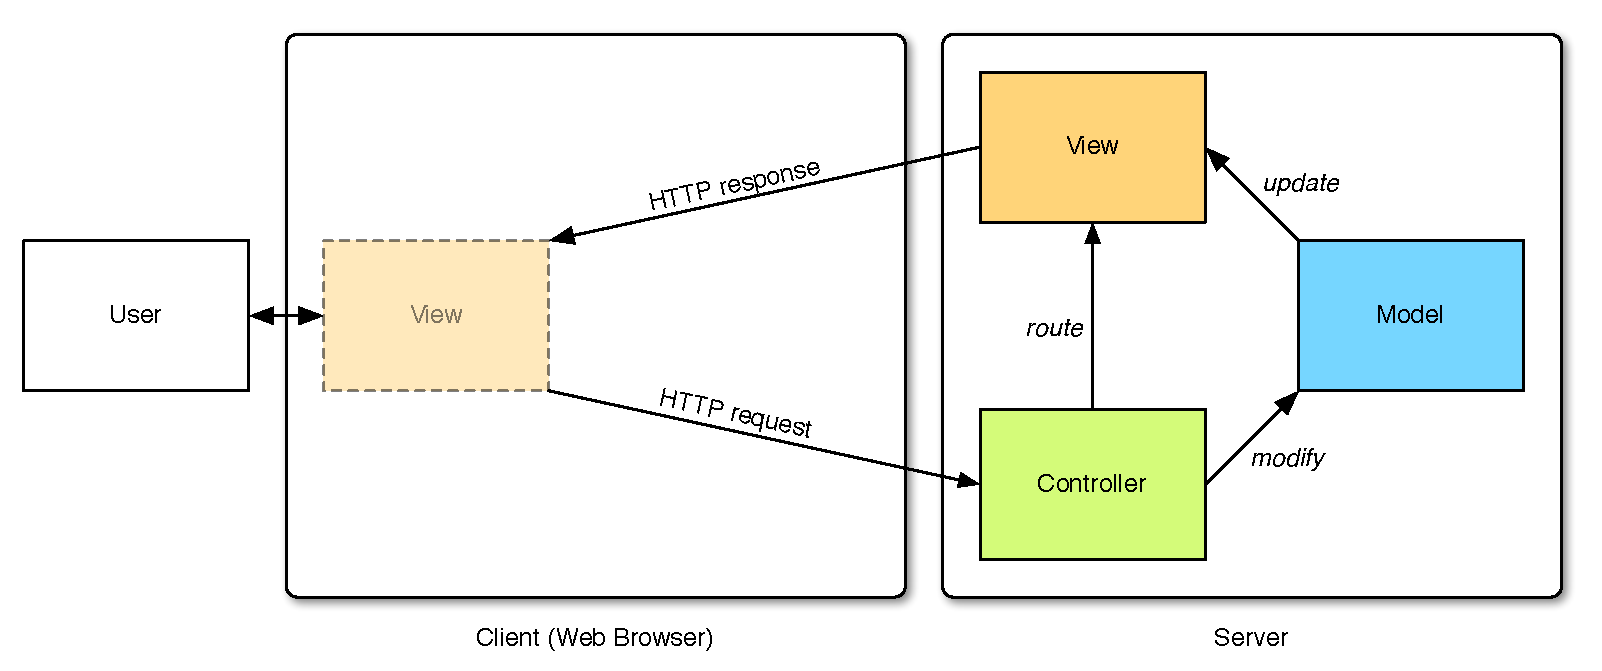
\includegraphics[width=16cm]{images/thinclientmvc.pdf}
	\caption{Structure of a Server Side MVC Architecture}
	\label{fig:thinclientmvc}
\end{figure}

The diagram reflects the sequence of control in this \ac{mvc} scenario. It is assumed that the server-side View is bound to a \ac{url}, and thus is the \ac{html} document to receive. Loading of a \ac{url} is always initiated by the user through the web browser.

The client-side View is displayed slightly transparent, as it is not a real \ac{mvc} View that gets data from a Model and performs actions through a Controller. It is the displayed version of the web page that was loaded in the browser, and it acts as a mediator between the user and the server (following \glspl{url} after the user clicks on links and displaying a web page after it is received). In later presented architectures, the Controller is mapped to a \gls{url} and invoked by the client-side Controller, instead of by the server-side View.

\subsubsection{Implementations}
% Implementations
Common implementations for this variant include \ac{mvc} frameworks for server-side programming languages:
\begin{description}
  \item[Struts] is an open source framework for building web applications using \ac{jee}. It implements a \emph{Model 2} architecture, as described in Section~\ref{sec:thinclient}. Struts uses a Servlet as the Front Controller to route requests to the actual Controller, which is responsible for a certain request. It responds with JSPs as Views and uses JavaBeans as Models.\footnote{See \url{http://struts.apache.org/}}

	\item[Ruby on Rails]--- or just \emph{Rails} --- is a \ac{mvc} web application framework for the Ruby programming language. It can make use of a variety of templating systems (eRuby, HAML and others) to construct Views. For the Models, Rails uses an object-relational wrapper on top of a relational database (such as MySQL, SQLite, DB2, and Oracle), but extended through plug-ins it can also use object databases for persistent storage of domain data.

	\gls{rails} ships the JavaScript framework \emph{Prototype}, which makes it possible to build \ac{ajax} applications using Rails as the backend, but Rails itself is a pure server-side \ac{mvc} framework.\footnote{See \url{http://rubyonrails.org/}}
\end{description}

\subsubsection{Applicability}
\begin{table}[H]
	\centering
	\begin{tabular}{l l}
\rowcolor{lightgray}
Criterion & Applicability\\
Data Model Complexity & \emph{Yes}\\
Real-time Model Synchronization & \emph{No}\\
Data Volume & \emph{No}\\
	\end{tabular}
	\caption{Applicability of a Server Side MVC Architecture}
\end{table}
The \emph{Server Side MVC Architecture} can be used for applications with a complex data model. As the pattern components reside completely on the server side, maintenance is easier to perform than if it was distributed. \ac{mvc} frameworks such as Struts, Spring, FLOW3, Rails and Synfony offer data modelling possibilities that are powerful enough to reproduce even very complex data models.

It is not suitable for real-time Model synchronization. Once sent to the client, the page cannot be updated --- it remains static. Providing real-time updates, or even non-real-time updates, would require a client-side mechanism to request and process subsequently sent data. Such mechanism is not present in a Server Side MVC architecture.

High data volume turns out to be a problem for this architecture, too. As data cannot be fetched after the site is loaded, all data that the user could want to process have to be loaded initially, and again with every navigational action the user might take. This results in high network traffic.

%=============================================================================
%=============================================================================
\newpage
\subsection{Distributed Controller MVC Architecture}
\label{sec:distcontr}
% General
The first change that can be made to the full server-side \ac{mvc} is to push the Controller to the client-side. This does not mean that there is no Controller on the server anymore, but its responsibility is reduced in comparison to a full server-side one. Thus, this \ac{mvc} web application architecture can be called \emph{Distributed Controller MVC Architecture}.

In Server Side MVC Architecture applications, navigational actions are bound to different pages. Refreshing a View requires to refresh the web page, and manipulating the Model is usually bound to calling a URL with POST or GET parameters --- which is the Controller's task.

In Distributed Controller MVC applications, the navigation is not only bound to different \emph{pages}. Still, pages can be accessed through the \ac{url} and lead to different main areas of the application. This task of routing is done by the server-side Controller\footnote{See p. \pageref{term:router} for more information on the connection between \emph{Controller} and \emph{Router} in web-based MVC applications.}.
The client-side part of the Controller, on the other hand, is encorporated by the possibility to interact with the web application \emph{without} changing the page (and thus loading a new \ac{url}) each time. It is realized as JavaScript code running in the browser, which is capable of handling minor navigational patterns within the page and delegating Model manipulation to the server--side Controller using \ac{ajax}. These tasks can include \gls{lazyloading} of content when scrolling or the creation of popup windows to display more detailed data.

Manipulations on the Model are initiated from the client-side Controller using an AJAX call, but are carried out by the server-side Controller code. This is usually a Servlet or a script, as described for Server Side MVC on page~\pageref{sec:thinclientmvc}. The server--side Controller needs to be able to analyze the AJAX request and act accordingly. The \emph{Distributed Controller MVC Architecture} does not maintain a client-side Model.

% Structure
\subsubsection{Structure}
The following architectural diagram (Figure~\ref{fig:distcontr}) illustrates the distributed Controller component.
\begin{figure}[H]
	\centering
	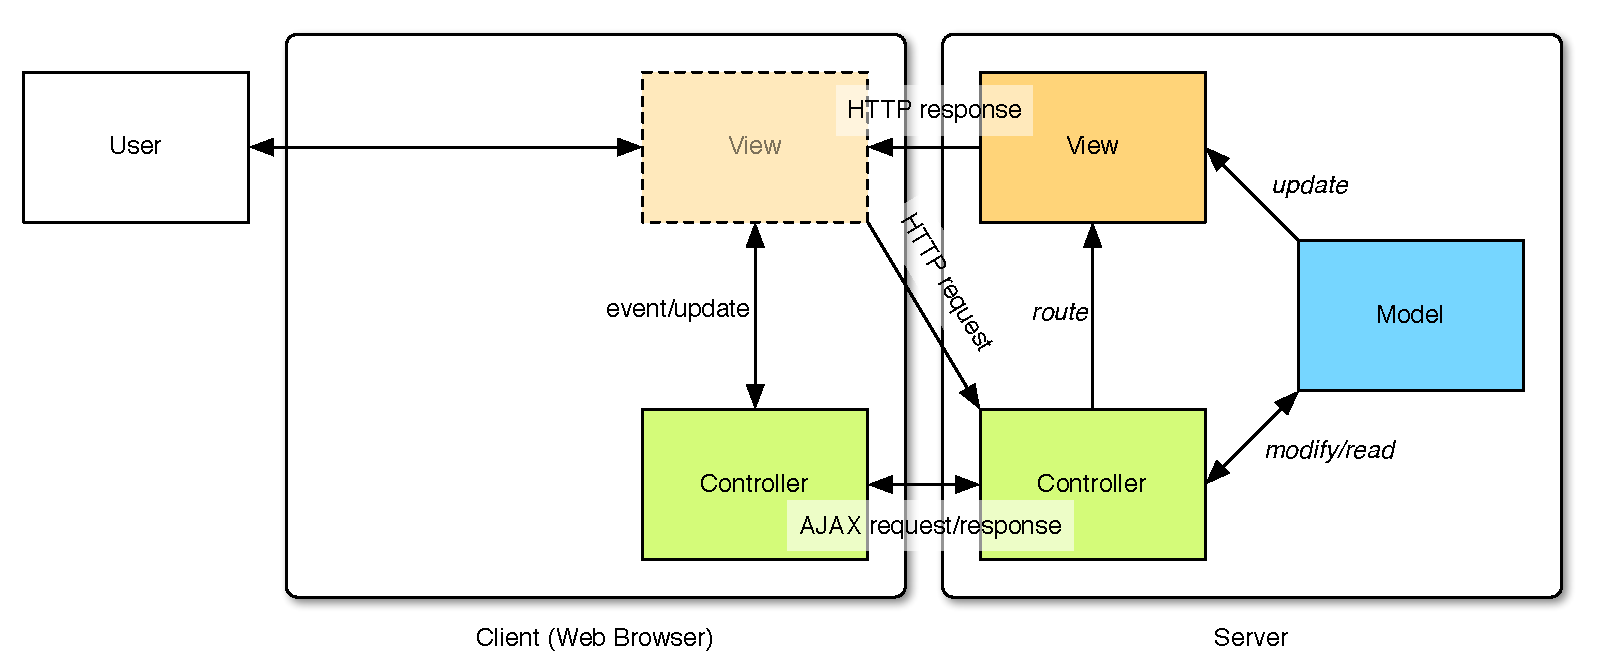
\includegraphics[width=16cm]{images/distcontrollermvc.pdf}
	\caption{Structure of a Distributed Controller MVC Architecture}
	\label{fig:distcontr}
\end{figure}

% Implementations
\subsubsection{Implementations}
The \gls{twitter} web application implements a Distributed Controller MVC Architecture, which is described by \citeasnoun{selvitelle}.

The application's main areas (``Home'', ``Connect'' and ``Discover'') as well as users' profiles have their own \acp{url}. Thus, the application has a server-side Controller. However, there is a lot of functionality that can be used without switching pages.

For example, when looking at a Twitter stream (or a search), you can scroll down to the bottom of the page, and additional (older) \glspl{tweet} are loaded. The respective event, in natural language ``the user scrolls to near the bottom of the page'', is processed by a client-side Controller, which then sends an \ac{ajax} request to the server and inserts the results (more Tweets) into the View (the list of Tweets, or \emph{stream}). This can be examined by logging the HTTP activity of Twitter.

According to \citeasnoun{venners}, the Twitter web application is based on Ruby on Rails as the server-side MVC framework.
For the client-side, there is no MV* framework used. Twitter only includes the jQuery JavaScript library, which is used for event handling and AJAX requests (client-side Controllers). This is proven by the JavaScript source code used by Twitter.

\subsubsection{jQuery Example}
To illustrate the interaction of client-side and server-side Controller, the following listings show how data from a form can be made persistent on the server without reloading the page. A simple task application using the JavaScript library \emph{jQuery} serves as an example.

\begin{listing}[H]
\begin{minted}[linenos=true,frame=no]{html}
<form>
  <input type="text" />
  <button type="submit">Add new Task</button>
</form>	
<ul>
  <li>Wash the dishes</li>
  <li>Do laundry</li>
  <li>Grocery shopping</li>
</ul>
\end{minted}
\caption{Task list HTML skeleton (View)}
\label{lst:taskhtml}
\end{listing}

The HTML skeleton in Listing~\ref{lst:taskhtml} contains a form with an input text field and a submit button, respectively. Also, it contains a list of items that represent already existing \emph{tasks}.

\begin{listing}[H]
\begin{minted}[linenos=true,frame=no]{javascript}
$('form button').click(function (event) {
  event.preventDefault();
  $.ajax({
    url: "newtask.php",
    data: {
      task: $('form input').val()
    }
  }).done(function() {
    $('<li>').html( $('form input').val() ).prependTo('ul');
    $('form input').val('').focus();
  });
});
\end{minted}
\caption{JavaScript-based client-side Controller for the task list}
\label{lst:taskjs}
\end{listing}

The JavaScript code in Listing~\ref{lst:taskjs} represents the client-side part of the Controller. An anonymous function is registered as a callback for the \emph{click} event of the form's submit button. In the callback itself, the default behaviour (that would be to submit the form) is prevented using \code{event.preventDefault();}. Then, an \ac{ajax} request is sent to the \ac{url} \pathname{newtask.php}, providing the text inside the form's input field as a parameter. By default, this is an asynchronous call using the \ac{http} GET method.

When the call returns successfully, another callback (the anonymous function inside the \code{\$.ajax().done()} invocation) adds the new task as a list item on top of the existing list. It then clears the input field and gives the keyboard focus back to it.

The \ac{php} code of the server-side Controller is not listed here. It would typically insert the given task into a database and return a unique ID, which then could be processed on the client.

% Twitter benutzt eine Mischugn aus diesem und dem nächsten

\subsubsection{Applicability}
\begin{table}[H]
	\centering
	\begin{tabular}{l l}
\rowcolor{lightgray}
Criterion & Applicability\\
Data Model Complexity & \emph{No}\\
Real-time Model Synchronization & \emph{Yes}\\
Data Volume & \emph{Depends}\\
	\end{tabular}
	\caption{Applicability of a Distributed Controller MVC Architecture}
\end{table}
The Distributed Controller MVC Architecture makes more use of client-side programming and thus is applicable for web applications that require more dynamicity on the client-side than the Server Side MVC Architecture.

The fact that this MVC distribution allows additional data loading without maintaining a client-side Model makes it a good choice for simple data structures. Complex Models, on the other hand, are harder to implement using the Distributed Controller MVC, as the missing client-side Model makes it impossible to manage data in a structured way. It is sufficient for the Twitter web application, as its data model is rather simple.

The client-side Controller allows loading data at any time, so it is possible to build applications with real-time data synchronization capabilities using a Distributed Controller MVC Architecture (although synchronization happens only from the server to the client in this case, as the client does not maintain a Model).

High data volumes can also be handled by this architecture. Using techniques like lazy loading, as Twitter does, data can be loaded on demand. However, depending on the amount of data and if the data should further be processed, an architecture with a client-side Model may be the better solution.

%=============================================================================
%=============================================================================

\subsection{Synchronized Model MVC Architecture}
% General
The next step towards a Rich Client is to bring the Model into the browser. In opposition to the Controller in the architecture discussed before, there is no distribution of Model responsiblity across the network nodes. Instead, the client-side Model is a copy, or an excerpt, of the original, server-side Model. The one in the browser is the operating Model --- all client-side manipulations are executed on the client-side Model. The server-side Model is used for persistence, which requires a synchronisation strategy between client and server.

The synchronisation strategy and possibilities of the client-side Model highly depend on what the Model represents.
\begin{itemize}
	\item If the client-side Model is an \emph{exact copy} of the server-side one (i.e. it keeps all the data that are also contained on the server-side), all Views and Controllers can directly interact with this exact Model. Synchronisation can happen
	\begin{itemize}
		\item periodically, i.e. after a defined amount of time (``timeout'')
		\item on special actions, e.g. manipulation of the client-side Model
	\end{itemize}
	It is recommended to only synchronize the differences between the client and server, usually called ``delta''.

	\item The client-side Model can also be only a \emph{partial copy} of the server-side one. By keeping track of which part of the data is already present on the client, data can be efficiently transferred from and to the server. This is preferred for high volumes of data. 

	The synchronisation strategies are the same as described above. Lazy loading can best be implemented using a partial client-side Model.
\end{itemize}

% Structure
\subsubsection{Structure}
\begin{figure}[H]
	\centering
	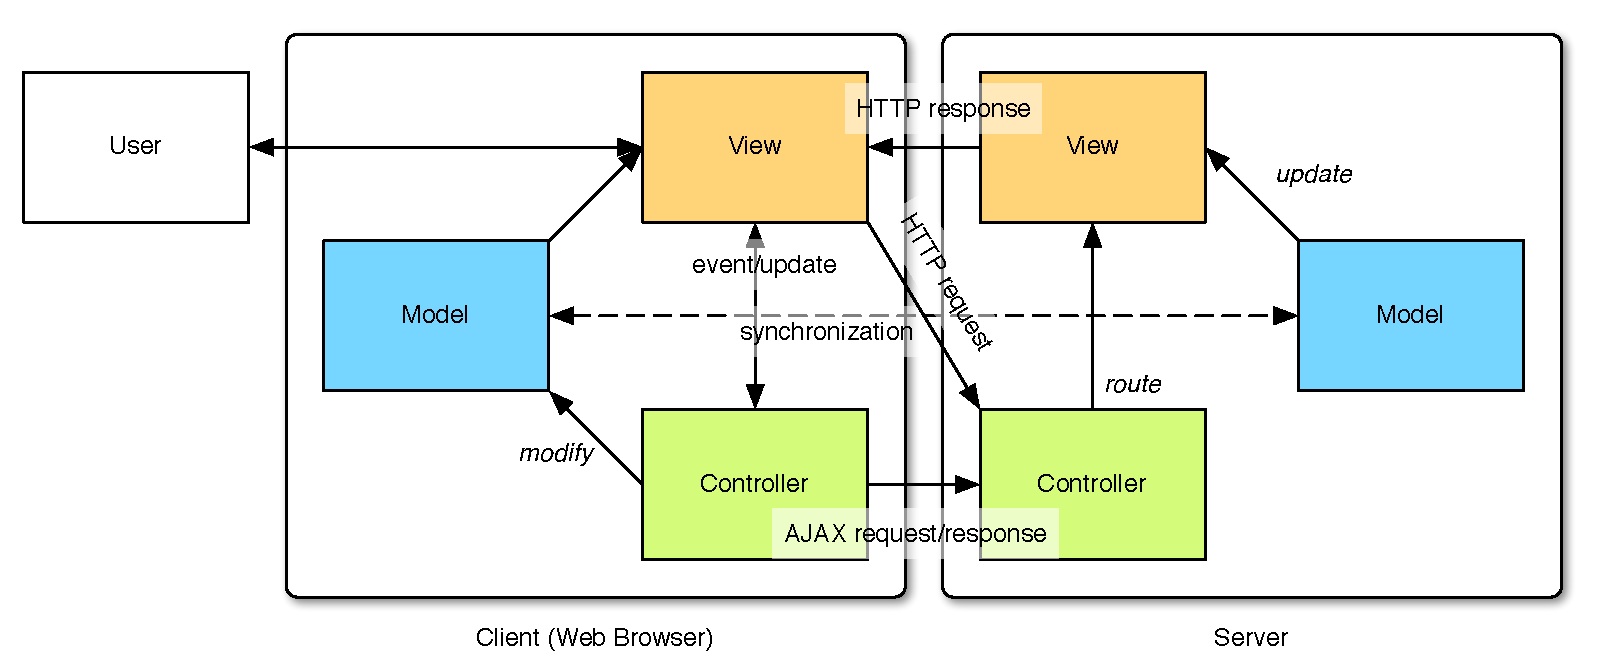
\includegraphics[width=16cm]{images/syncmodelmvc.pdf}
	\caption{Structure of a Synchronized Model MVC Architecture}
	\label{fig:syncmodel}
\end{figure}

In this architectural diagram, the synchronization between the client-side and server-side Models is illustrated using a dashed line.

\subsubsection{Implementations}
Once Model synchronisation is part of the architecture, a client-side MV* framework is often used to structure the JavaScript code; this is especially useful, as basic functionality for synchronisation and data I/O do not have to be implemented manually, but are provided by most frameworks.

There are a lot of examples that make use of the Backbone.js framework. The open-source social network \emph{Diaspora}\footnote{See \url{https://joindiaspora.com/}}, for example, uses Ruby on Rails as a server-side MVC framework, and in parallel Backbone.js on the client-side. Although Ruby on Rails follows MVC and Backbone.js is built after MVP, these two frameworks work together well.

Backbone.js Models can directly synchronize with Rails Models without any further transformations, as they can be configured to use the same JSON format for data exchange.

One can argue that the presence of a complete MV* triad on the client makes the server-side Controller obsolete: it is no longer needed to manipulate the server-side Model. This is correct for completely client-sided MV* applications, as described in the next section (\emph{Rich Client MVC}). Rich Client MVC applications are one-page applications, which means that their user interface and routing is handled completely using JavaScript. But in applications following the Synchronized Model architecture, both routing and initial creation of the user interface happens on the server-side.

Another advantage of the server-side Controller is the fact that multiple front-ends can be built to collaborate with the server. In addition to the web client, mobile clients that follow a thin client paradigm --- for example for performance reasons --- can make use of the completeness of server-side MVC.

\subsubsection{Applicability}
\begin{table}[H]
	\centering
	\begin{tabular}{l l}
\rowcolor{lightgray}
Criterion & Applicability\\
Data Model Complexity & \emph{Depends}\\
Real-time Model Synchronization & \emph{Yes}\\
Data Volume & \emph{Yes}\\
	\end{tabular}
	\caption{Applicability of a Synchronized Model MVC Architecture}
\end{table}

% Complexity
The parallel structure of a Synchronized Model MVC Architecture makes the handling of comples data models difficult. Data can be changed on two different points in the application: on the client, using the client--side Controller, and on the server, using the client--side Controller to send an AJAX request to the server--side Controller, which then modifies the Model. Of course it is possible to efficiently resemble complex data models with this architecture variation, but with a lot of Models and cross-references included, it is possible that the structure becomes intransparent.

%Due to the parallel architecture of Synchronized Model MVC, handling complex Models may need high effort, as suitable Views have to be built on both the client-side and server-side. Changes have to be made on both sides, too. A possible solution would be to implement modules in a format that can be used by both the client-side and the server-side code. This can include a templating language understood by both a JavaScript framework and the programming language used on the server. Another approach is to use JavaScript for both server and client code, for example using the server-side JavaScript platform \emph{Node.js}\footnote{See \url{http://nodejs.org/}}.

% Real-time
The synchronization of the Model makes applications with real--time snychronization possible, even for more complex data structures. Using the techniques described as \emph{\gls{comet}} and WebSockets on page \pageref{term:comet}, every synchronization strategy can be implemented, whether the client-side Model is a complete or only a partial copy of the server-side Model.

% Data Volume
This architecture is suitable for processing high data volumes, for the same reason as it is suitable for applications that require real-time data synchronization. As the Model is synchronized between client and server, it is possible to only load the required data onto the client-side and load additional data subsequently, on demand.

%=============================================================================
%=============================================================================

\subsection{Rich Client MVC Architecture}
The Rich Client MVC Architecture is described as  ``RIA Architecture''\glsunset{ria}\footnote{RIA is short for \emph{Rich Internet Application}. The term can be used for rich web clients, but it usually describes applications developed with Adobe Flash or Flex, see Section~\fullref{sec:terminology}} by \citeasnoun{steele}. It places the whole set of Model, View and Controller on the client-side, while only a Model stays on the server-side.

What distinguishes this variant from the \emph{Synchronized Model MVC Architecture} is that there is no server-side View or Controller anymore. Of course, there is an entry point to the application needed. This is usually an almost empty \ac{html} file that only contains a skeleton and references to additional resources, such as JavaScript, CSS and image files that have to be loaded subsequently. The user interface is being constructed on the client side, purely through JavaScript code.

\subsubsection{Structure}
\begin{figure}[H]
	\centering
	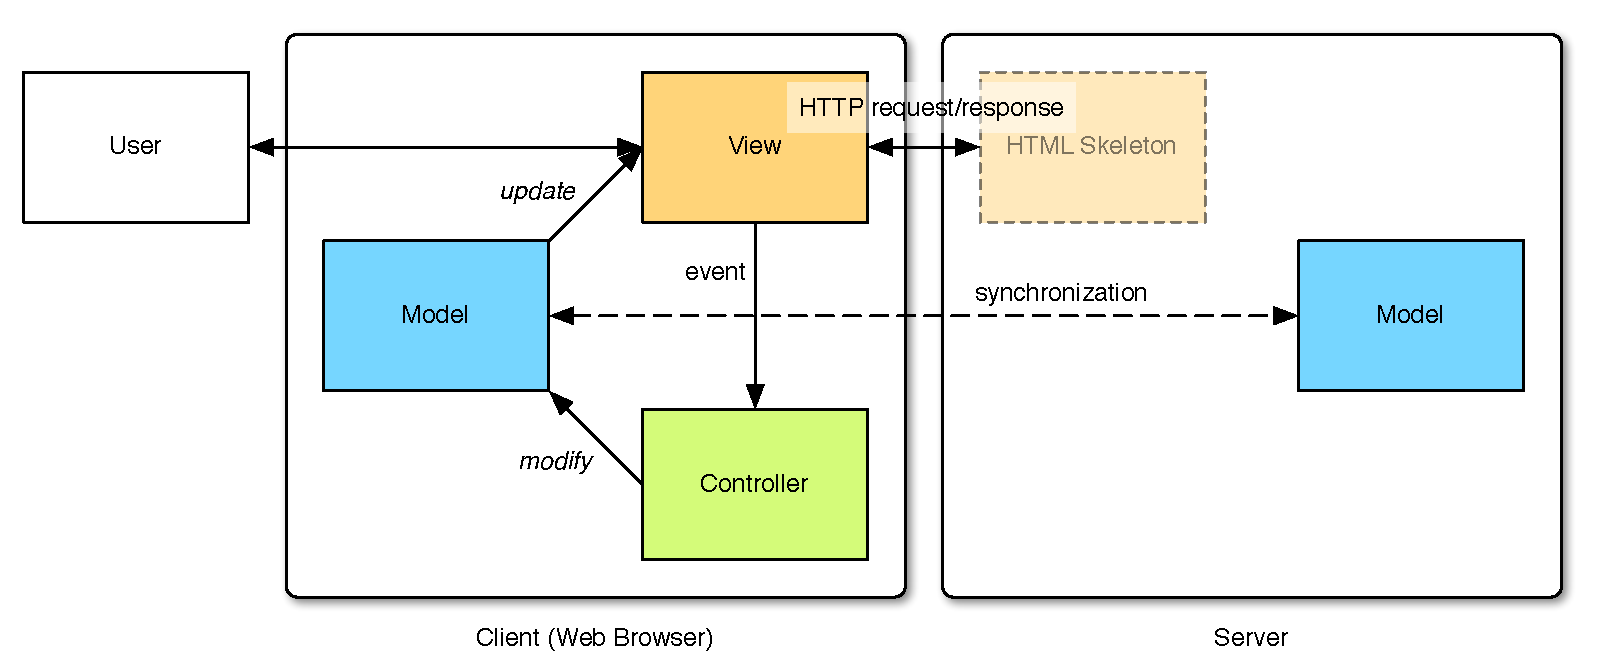
\includegraphics[width=16cm]{images/richclientmvc.pdf}
	\caption{Structure of a Rich Client MVC Architecture}
	\label{fig:richclientmvc}
\end{figure}

\subsubsection{Implementations}
The Dojo Toolkit\footnote{See \url{http://dojotoolkit.org/}} comes with a great variety of different modules and widgets (called \emph{Dijits}). Dojo 1.6\footnote{Please note that Dojo developed various \ac{mvc} approaches over time, and they differ quite a lot between versions 1.8 (the latest as of September 2012) and older ones. Dojo 1.7 provides the \pathname{dojox.mvc} package, but in this thesis, Dojo 1.6 is the version referred to, as it is the version used by \ac{ibm} \nexus\ at this time.} makes it possible to build pure client-side \ac{mvc} applications.

In Dojo, the Model is a Dojo Data Store, for example \code{dojo.store.Memory} and \code{dojo.data.ItemFileReadStore}. Using the \code{dojo.store.Observable} wrapper around the store, the Observer pattern can be established between View and Model. Views can be Dijits, either Dojo's own or custom ones. Controllers can be implemented as own modules, but often Controller code is put inside of the Dijit, which breaks with the \emph{Separation of Concerns} paradigm of \ac{mvc}.

Using the \code{dojox.data.JsonRestStore}, a RESTful web service can be connected to the client-side store, which allows data persistence on the \acs{rest} server and makes a Rich Client/Thin Server configuration possible.
Dojo's \ac{mvc} implementation is further discussed in Chapter~\fullref{chap:nexus}.

\subsubsection{Applicability}
\begin{table}[H]
	\centering
	\begin{tabular}{l l}
\rowcolor{lightgray}
Criterion & Applicability\\
Data Model Complexity & \emph{Yes}\\
Real-time Model Synchronization & \emph{Depends}\\
Data Volume & \emph{Yes}\\
	\end{tabular}
	\caption{Applicability of the Rich Client MVC Architecture}
\end{table}

A web application with a Rich Client MVC Architecture is able to handle complex data models. The most important requirement for this is a well-defined interface between the client-side and server-side Models. As the code to process and consolidate Model data is situated on the client-side only, even very complex domain data can be handled by this application architecture.

The Rich Client MVC architecture is suitable for real-time model synchronization, as long as a powerful modern web browser is used. This requirement has two reasons:
\begin{itemize}
	\item Depending on the complexity and the number of Models to synchronize, the \emph{Comet} technique described on page~\ref{term:comet} might not be feasible anymore. Too many iframes or pending requests in parallel can slow down the user interface. Using a modern browser that supports HTML5, WebSockets can be used for synchronization, which also allow more control over the data transfer.
	\item Due to the fact that the whole application is situated on the client-side, a lot of memory might be needed. Also, the execution time of JavaScript code can be slow if the JavaScript engine is not capable enough to run a full-fledged, desktop-level web application.
\end{itemize}

Regarding data volume, the same is true for Rich Client MVC as it is for a Synchronized Model MVC architecture.

%=============================================================================
%=============================================================================
%\newpage
\subsection{Comparison and Conclusion}

The results of the applicability evaluation are summarized in Table~\ref{tab:comparison}.

\begin{table}[H]
	\centering
	\begin{tabular}{l p{2.4cm} p{3cm} p{3cm} }
\rowcolor{lightgray}
MVC Architecture & Data\ Model Complexity & Real-time Model Synchronization & Data Volume\\
Server Side & \cellcolor{green}\emph{Yes} & \cellcolor{red}\emph{No} & \cellcolor{red}\emph{No}\\
Distr. Controller & \cellcolor{red}\emph{No} & \cellcolor{green}\emph{Yes} & \emph{Depends}\\
Synchr. Model & \emph{Depends} & \cellcolor{green}\emph{Yes} & \cellcolor{green}\emph{Yes}\\
Rich Client & \cellcolor{green}\emph{Yes} & \emph{Depends} & \cellcolor{green}\emph{Yes}\\
	\end{tabular}
	\caption{Applicability of the different MVC architectures}
	\label{tab:comparison}
\end{table}

Both the Server Side and Rich Client MVC architecture are characterized by their rather simple structure. This fact makes them preferable for applications with complex data models, as the data have to be modeled only on one of the two tiers.
For applications that need to process data in real-time or large amounts of data, the three architectures based on AJAX are suitable. They allow loading of data at virtually any time during execution of the application and can use techniques like \emph{lazy loading}.
\chapter{MVC in IBM Content Navigator}
\label{chap:nexus}
This chapter introduces the IBM Content Navigator application and framework. After an overview on its architecture and plug--in system, the main client-side components Dojo and \ac{idx} are outlined. To conclude this chapter, the design and implementation of a log analysis plug--in is discussed.
\section{Architecture and Extension Points}
IBM Content Navigator is an enterprise web application written in Java and JavaScript. The server--side part is designed to run on a \ac{j2ee} application server, the client--side part runs in a web browser. The architecture of Content Navigator, which is presented here, allows the extension through plug--ins at many points of the application.

\subsection{Architecture: Layers and Components}
IBM Content Navigator is designed after the \emph{Separation of Concerns} principle. This is true for the different layers of Content Navigator on the one hand, and the different tiers it uses on the other hand. The layers of ICN are shown in Figure~\ref{fig:nexuslayers}.

\begin{figure}[H]
	\centering
	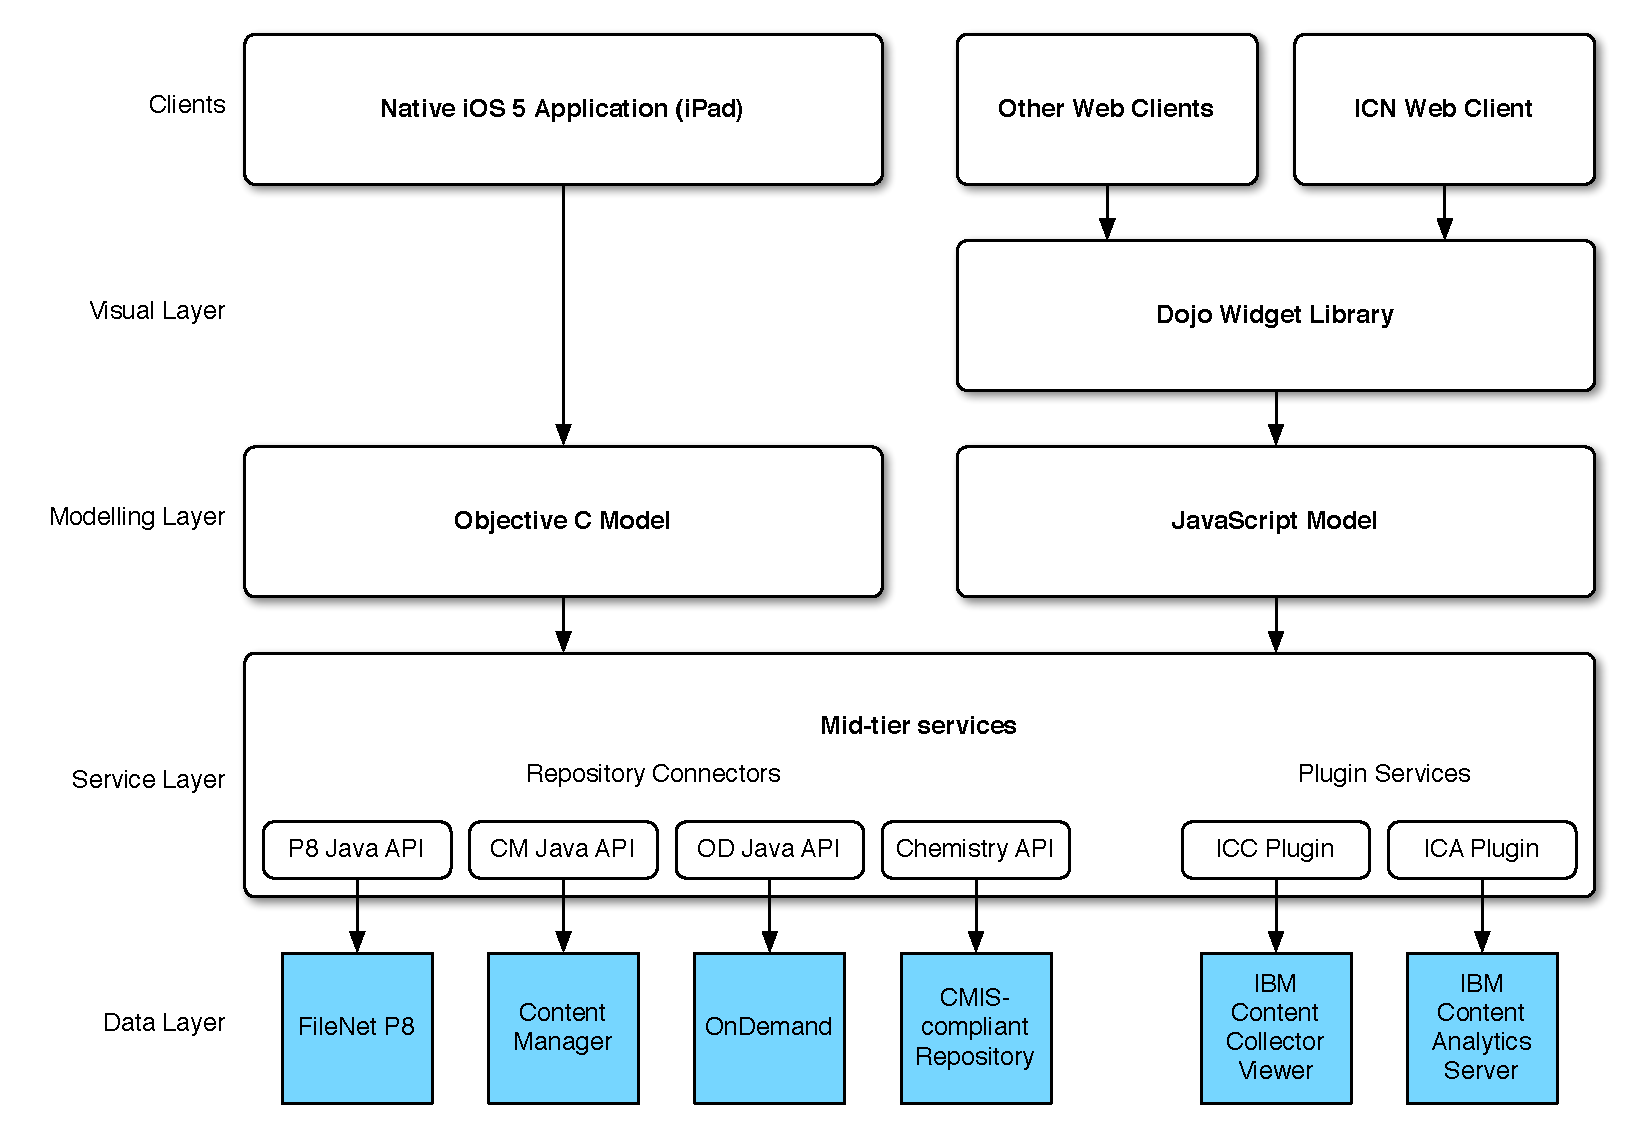
\includegraphics[width=16cm]{images/layers.pdf}
	\caption{Layers of IBM Content Navigator}
	%\captionsetup{font={footnotesize,bf,it}}
	%\caption*{Source: \cite[p. 5]{gof}}
	\label{fig:nexuslayers}
\end{figure}

The top layer represents the actual clients for Content Navigator. Besides the desktop web client, there exists also a mobile iOS 5 client, which is not in the scope of this thesis. The client layer makes use of the visual layer underneath that contains all the Dojo widgets (\emph{Dijits}). In turn, the widgets access the modelling layer, which contains JavaScript Models held in the browser. On the one hand, these models can be connected to mid-tier services, such as ECM repository \glspl{api}, on the other hand, they can be directly connected to external, HTTP-based services, such as \ac{rest}.

The mid-tier services are implemented in Java and run on the application server, whereas the modelling and widget layers run in the browser. This is illustrated by Figure~\ref{fig:nexustiers}, which shows the tier architecture of Content Navigator.

\begin{figure}[H]
	\centering
	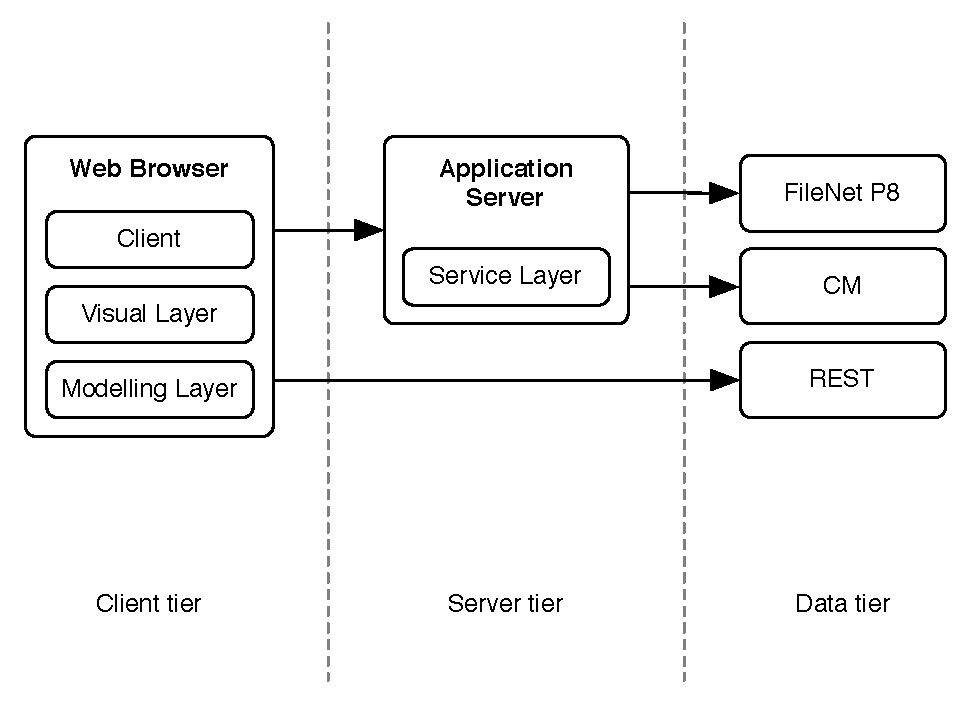
\includegraphics[width=14cm]{images/tiers.pdf}
	\caption{3-Tier architecture of IBM Content Navigator}
	%\captionsetup{font={footnotesize,bf,it}}
	%\caption*{Source: \cite[p. 5]{gof}}
	\label{fig:nexustiers}
\end{figure}

\subsection{Extension Points: Plug--ins}
\label{sec:plugincomponents}
The modular architecture previously presented makes it easy to extend Content Navigator on different levels. Plug--ins for \ac{icn} can include different components that can directly be used inside of \ac{icn}, as described by \citeasnoun**[pp. 103ff.]{redbook}. The ones relevant for the log analysis plug--in are \emph{Plugins} themselves, \emph{Features} and \emph{Widgets}.

\begin{description}
	\item[Plugins] are the containers for the following extension points, which are registered with ICN through the ``Plugin'' Java class.
	\item[Actions] are buttons or menu items that can be triggered by the user; they can be added to the existing \ac{ui} of ICN.
	\item[Menus] of the existing UI can also be created and customized, just like \emph{Actions}.
	\item[Plug--in Services] allow developers to extend the service layer of Content Navigator. They can implement arbitrary Java code, but can be called from the client-side JavaScript as they are exposed by a Servlet.

	Using a \emph{Service}, it is possible to build anything that Java is capable of. This can be, just to name a few examples, a proxy for REST calls, an additional connector to a content repository not already covered by ICN, or a system to save data on the server side. The \ac{ica} plug--in uses \emph{Services} to connect to an ICA server via \ac{sso}.
	\item[Features] are areas of the application \ac{ui}. In ICN, the Browser, Favorites, Team Spaces, Search, Work and Administration \emph{Features} do already exist and can be accessed using the Feature Pane on the left side of the \ac{ui} (when logged in).

	\emph{Features} are associated with a Dojo class to specify the View that should be shown when the \emph{Feature} is accessed.
	\item[Viewers] are used to display the content of a specific document type.
	\item[Layouts] can customize the overall layout of the application \ac{ui}, whereas \emph{Features} can only define a certain application area. ICN's standard layout (Banner Bar at the top, Global Menu below, Feature Pane on the left and Features filling the remaining screen space) can be changed using \emph{Layouts}.
	\item[Request and Response Filters] are used to change the JSON sent from and received by \emph{Services}.
	\item[Widgets] are Dojo Dijits that can be included in Plug-ins. They can either be developed from scratch or extend already existing Dojo or IDX Dijits. More on Dijits is written in Section~\ref{sec:dojo}.
\end{description}

Besides these components, arbitrary JavaScript code, best created as Dojo modules, can be written and packaged into the plug--in. This includes Model and Controller code. Figure~\ref{fig:plugincomponents} illustrates the connection between extension points and the ICN layer architecture (please compare to Figure~\ref{fig:nexuslayers}).

\begin{figure}[H]
	\centering
	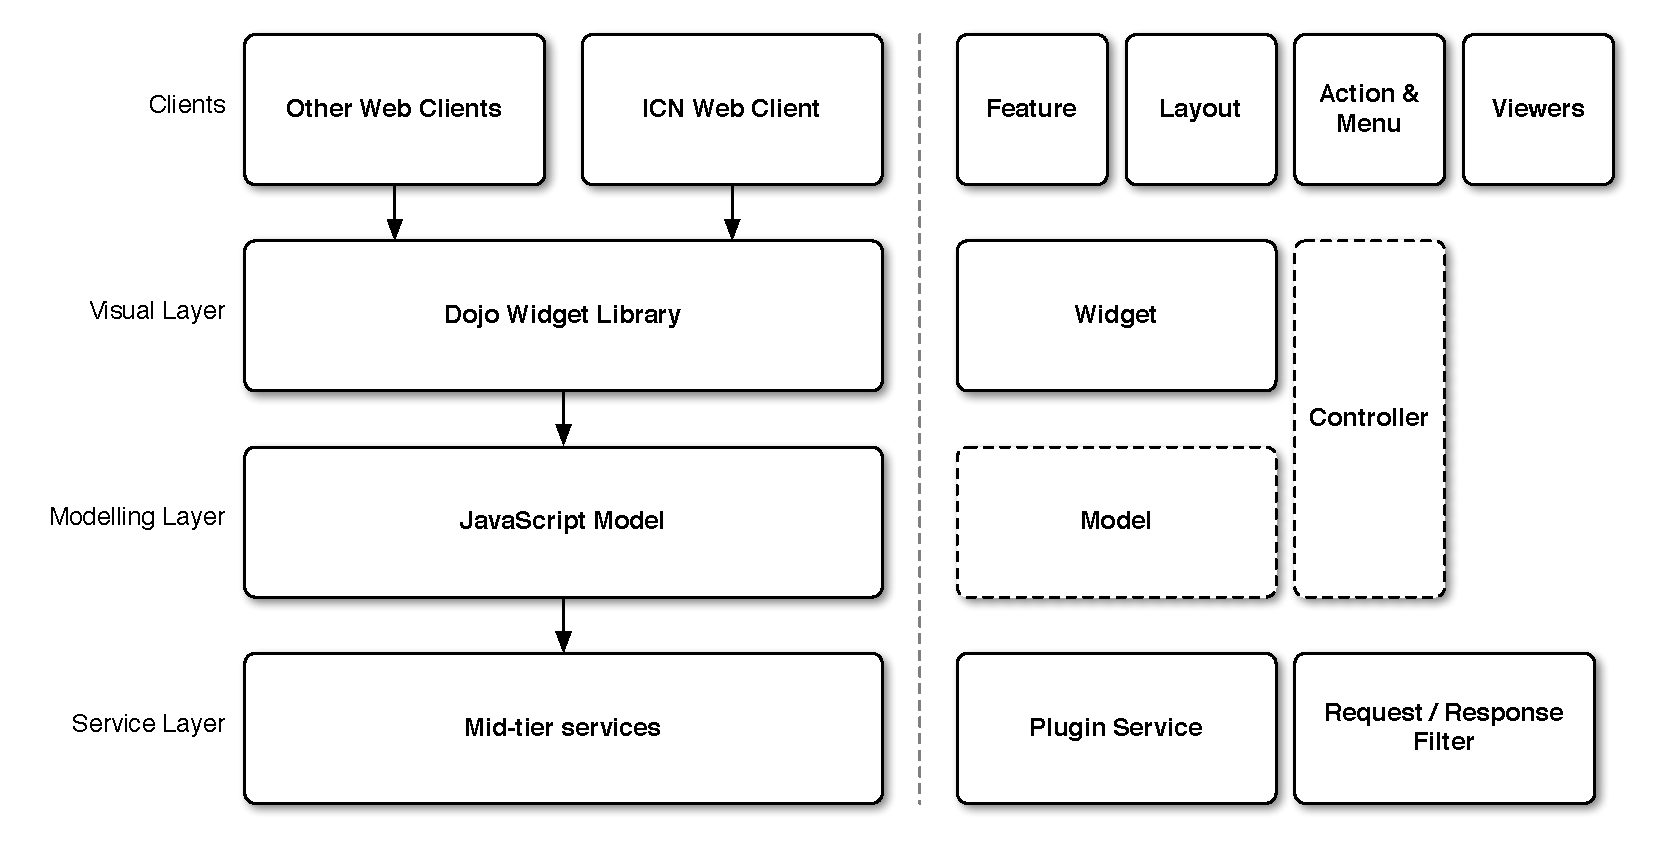
\includegraphics[width=16cm]{images/plugincomponents.pdf}
	\caption{Plug--in components extending ICN}
	\label{fig:plugincomponents}
\end{figure}

As can be seen, plug--ins cannot extend the data layer, as it is not part of \acl{icn} itself, but rather composed of external data sources, such as content repositories and REST services.

\subsection{Deployment and Configuration}
Content Navigator itself is packaged --- without any plug--ins --- into an \ac{ear} file and can directly be deployed on an application server, such as IBM \acl{was}. The connection to a \gls{db2} database for storing and loading the configuration is needed and can be set up using the ICN initialization tool.

Plug--ins are deployed separately. They are packaged as \ac{jar} files and placed at any location that is accessable via a \ac{url}. Plug--ins can be loaded using the administration pane of \ac{cn}. This separation between the actual application and its plug--ins allows the application administrator to update, load and unload plug--ins without restarting \ac{cn} or the application server.

Different ICN-based applications, called \emph{Desktops}, can run on the same ICN installation. A Desktop can be configured using the ICN administration pane; it is assigned a \emph{Layout} and a number of \emph{Features} (as described in Section~\ref{sec:plugincomponents}), as well as content repositories and other options. A Desktop is chosen via the URL, for example \code{http://localhost/navigator?desktop=sccm}. Figure~\ref{fig:nexusapps} illustrates how applications can be assembled using \emph{Features} of different plug--ins.

\begin{figure}[H]
	\centering
	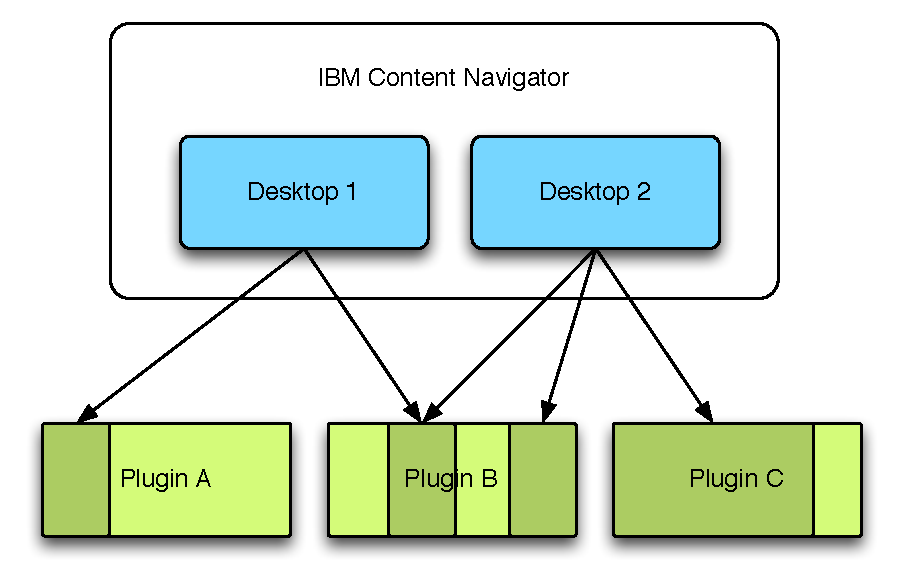
\includegraphics[width=10cm]{images/nexusapps.pdf}
	\caption{ICN Applications using different Plug--in Features}
	\label{fig:nexusapps}
\end{figure}

\section{Dojo Model--View--Controller}
\label{sec:dojo}
This section introduces the components of Dojo that are relevant to building \acl{mvc} applications, and those that were especially used while building the log analysis plug--in for \ac{sccm}. As IBM Content Navigator 2.0 (which is the latest version as of September 2012) includes Dojo 1.6, this is the version of Dojo referred to in this section.

\subsection{Dojo Basics}
The Dojo Toolkit, usually just called \emph{Dojo}, is a set of libraries to build JavaScript applications. In opposite to other JavaScript libraries, such as jQuery, Prototype or Mootools, Dojo is not only aimed at simplifying \ac{dom} manipulation, \ac{ajax} and event handling, but also comes with an extensive widget library (\emph{Dijit}) and graphics/charts \ac{api}.

Dojo is separated into three packages:
\begin{description}
	\item[Dojo] is the core package and contains basic functionality, such as \ac{dom} manipulation, \ac{ajax}, effects, and JavaScript language helpers. Its \gls{namespace} is \code{dojo}.
	\item[Dijit] contains all stable widgets, such as layout widgets, forms, dialogs, and a tree view. Its namespace is \code{dijit}.
	\item[DojoX] are the Dojo extensions in the namespace \code{dojox}. This package contains less common components, such as the graphing and charting \ac{api}. The DataGrid (\code{dojox.grid.DataGrid}) and JsonRestStore (\code{dojox.data.JsonRestStore}), which are part of DojoX, are further discussed in Section~\ref{sec:loganal}.
\end{description}

% TODO: eventuell Dojo module beschreiben?

\subsubsection{Classes and Objects}
JavaScript is a prototype-based object-oriented programming language. Dojo simulates class-based object orientation, which is more familiar to developers used to Java, C++, C\# and other languages. To illustrate this, Listing~\ref{lst:classes} contains the declaration of a Dojo class using \code{dojo.declare}.

\begin{listing}[H]
\begin{minted}[linenos=true,frame=none]{javascript}
dojo.declare("my.Thinger", null, {
  constructor: function(/* Object */args){
    dojo.safeMixin(this, args);
  }
});
\end{minted}
\caption{Declaring a Dojo class}
\label{lst:classes}
\end{listing}

This listing declares the \code{my.Thinger} class (in the \code{my} namespace). When instantiating an object, the constructor mixes the \code{args} argument, which should be a JavaScript object, into the new instance. The result of this mixin is shown in Listing~\ref{lst:mixin}.

\begin{listing}[H]
\begin{minted}[linenos=true,frame=none]{javascript}
var thing = new my.Thinger({ count:100 });
console.log(thing.count);
\end{minted}
\caption{Instantiating an object using a Dojo class}
\label{lst:mixin}
\end{listing}

The object\footnote{JavaScript objects can simply be created as literals. Object literals are enclosed in braces (`\{' and `\}') and contain a comma-separated list of properties (attributes and methods).} provided as an argument to the \code{my.Thinger()} constructor is mixed into the new object \code{thing}. This means, that \code{thing} now contains the properties of this object, which can be proven by printing out \code{thing.count} in the console.

All Dojo components, including Dijits, are created using this concept, and so are the classes developed for the log analysis plug--in.

\subsubsection{Scope}
Another of Dojo's concepts being of help in \ac{mvc} applications and the plug--in is \code{dojo.hitch}. The JavaScript \ac{api} of web browsers features a callback-based event system. This means that callbacks are registered to an event and triggered when the event occurs. A frequently faced problem is that the \gls{callback} function has a different scope than the developer would expect \cite[pp. 53--56 and pp. 180--185]{flanagan}. In JavaScript, this is typically solved using a \emph{closure}, a concept to pass on a given scope to another function. In applications with a lot of callbacks, which may also be depending on each other to execute, closures can have a negative impact on the code maintainability and comprehensibility. \code{dojo.hitch} returns a function that, when executed, has a specified scope, as shown in Listing~\ref{lst:hitch}.

\begin{listing}[H]
\begin{minted}[linenos=true,frame=none]{javascript}
function myCallback() {
  console.log(this.localVariable)
}

dojo.declare("my.Thinger", null, {

  localVariable: "I am in the Thinger scope",
  button: null,

  constructor: function() {
    this.button = new dijit.form.Button({
      label: "Hello"
    });
    dojo.connect(this.button, 'onClick', dojo.hitch(this, myCallback));
  }
});

var thing = new my.Thinger();
\end{minted}
\caption{Instantiating an object using a Dojo class}
\label{lst:hitch}
\end{listing}

This listing first defines a function that acts as a callback and refers a variable (``localVariable'') of its own scope (``this''). The Dojo class declared below introduces said variable and constructs a button. In line 14, the ``onClick'' event is registered with the callback through \code{dojo.hitch(this, myCallback)}. It means that the scope of \code{myCallback} at execution time of the callback is set to what \code{this} has been in line 14.
\subsection{MVC Components}
Dojo provides different components that make it possible to build applications using a MVC architecture. In opposition to JavaScript frameworks that were built towards \emph{structuring} an application using MVC (or a comparable pattern), such as Backbone.js, Ember.js and JavaScriptMVC, Dojo lets the software engineer decide on the architecture.

\subsubsection*{Model}
The modules \code{dojo.data} and \code{dojox.data} provide the data modelling layer. They contain a number of Model equivalents, called \emph{Stores}, all of which implement one or more interfaces to handle data \cite{zyp}:
\begin{itemize}
	\item The \emph{Read API} forces the Store to provide methods and maintain internal structures to expose a Store's data
	\item The \emph{Write API} enables a Store to accept data manipulations
	\item The \emph{Identity API} forces the Store to manage an identifier for each single data item. It must be possible to look up a data item using this unique identifier.
	\item If implementing the \emph{Notification API}, other objects can connect to events that fire when data in the Store are changed (an implementation of the \emph{Observer} pattern).
\end{itemize}

Dojo already implements various stores that serve different purposes and can use a specific data source. The \code{ItemFileReadStore}, for example, takes a file of \ac{json} data as the data source (specified by a \ac{url}). It implements the \emph{Identity} and \emph{Read} APIs, so data can be read, but not written. As the source is a file and data cannot be manipulated, it is not necessary for this store to implement the \emph{Notification} API.

The \code{JsonRestStore} serves a more complex purpose. It is connected to a \ac{rest} service and thus needs to implement both the \emph{Read} and \emph{Write} APIs. But the other two APIs are implemented also --- this is especially important as this store is often used in cooperation with a Dijit, such as the Tree or DataGrid. To keep the Dijits up to date, a notification mechanism as provided by the \emph{Notification API} is necessary (see next section for more information on the Tree and DataGrid).


\subsubsection*{View}
In Dojo, the View usually is a single Dijit or a collection of interrelated Dijits. This section presents two data-centric Dijits that are part of Dojo 1.6.

The \emph{Tree} (\code{dijit.Tree}) is a Dijit to display hierarchical data. It cannot connect directly to a Dojo store, but needs an additional API to handle the nested data model. These API can either be implemented manually by mixing in the according functions into the store when instantiating it, or the store can be wrapped by either one of the already existing \code{TreeStoreModel} and \code{ForestStoreModel}. The first expects a single root item, whereas the second expects multiple root items (thus the name \emph{Forest}).

\begin{figure}[H]
	\centering
	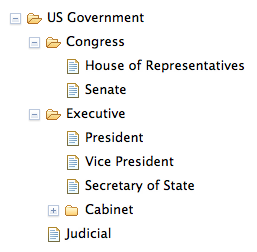
\includegraphics[width=6cm]{images/tree.png}
	\caption{Screenshot of a Dojo Tree}
	%\captionsetup{font={footnotesize,bf,it}}
	%\caption*{Source: \url{http://dojotoolkit.org/documentation/tutorials/1.6/store_driven_tree/}}
	\label{fig:tree}
\end{figure}

Listing~\ref{lst:tree} shows the creation of a store, a TreeStoreModel wrapper around that store and a Tree connecting to the store via the TreeStoreModel. A REST service at the URL \code{data/} is presumed, and the data returned must have a special structure: the attribute ``name'' has to be present in every item, as it is used as the label, and an array with child items has to be placed unter the ``children'' attribute.

Listing~\ref{lst:treejson} shows a sample JSON structure that is returned by the REST service at \code{data/}.

\begin{listing}[H]
\begin{minted}[linenos=true,frame=none]{javascript}
dojo.require("dijit.Tree");
dojo.require("dojox.data.JsonRestStore");
dojo.require("dijit.tree.TreeStoreModel");

store = new dojox.data.JsonRestStore({
  target: "data/"             // URL to the REST service
});

treeModel = new dijit.tree.TreeStoreModel({
  store: store,               // the store to wrap around
  query: {tree:"root"},       // root item
  labelAttr: "name",          // name of the label attribute
  childrenAttrs: ["children"] // attributes holding children
});

tree = new dijit.Tree({       // create a tree
  model: treeModel            // give it our model
}, "tree");                   // target HTML element's id

tree.startup();
\end{minted}
\caption{Creating a Tree with a store and TreeStoreModel}
\label{lst:tree}
\end{listing}



\begin{listing}[H]
\begin{minted}[linenos=true,frame=none]{javascript}
{
  name: "World",
  children: [
    { name: "Africa" },
    { name: "Australia" },
    { name: "Asia" },
    { name: "Europe" },
    { name: "North America",
      children: [
        { name: "Canada" },
        { name: "USA" }
      ]
    },
    { name: "South America" }
  ]
}
\end{minted}
\caption{Sample JSON data for the Tree Dijit}
\label{lst:treejson}
\end{listing}

The \emph{DataGrid} (\code{dojox.grid.DataGrid}) is a Dijit to display tabular data, similar to a spreadsheet. It can be used to display high amounts of data, using features like editable cells, custom cells that contain Dijits or arbitrary HTML code, and lazy loading. Its extension \code{dojox.grid.TreeGrid} can even display hierarchical tabular data using expanders and aggregates.

In opposition to the Tree, the DataGrid can directly access the data of a store. That store has to implement at least the \emph{Read} and \emph{Identity} APIs. The DataGrid also needs a \emph{structure}, which is an object describing the cells of the grid and the source of the cells' data. In the simplest case, a cell can contain the value of an attribute of the according item, but the cell content can also be custom, for example a Dijit or an image.

As the DataGrid is one of the most frequently used Dijits in the log analysis plug--in that was developed in the course of this thesis, an extensive example of implementing it is given later in Section~\ref{sec:plugindesign}.

In Dojo, a View can also be completely built by hand. An example for that is shown in Section~\ref{sec:customview}: a simple, data-displaying IDX Dijit is taken and methods are added to connect it to a Dojo store.

\subsubsection*{Controller}
For the Controller, Dojo does not provide any special classes or APIs. The Controller code can be any code that binds callbacks to View events and performs updates on one or more Models.

An example of a Controller is given in Section~\ref{sec:customview}, which shows the implementation of a custom Model--View--Controller triad using Dojo and the IDX Dijit \code{idx.grid.PropertyGrid}.
%=============================================================================
%=============================================================================
\newpage
\section{Implementation of a Log Analysis Plug--in}
\label{sec:loganal}
In the context of this Bachelor's thesis, a log analysis system was developed by two students. The author created a front-end using \acl{icn}, whereas \citeasnoun{metzger} implemented the respective back-end using \ac{ibm} BigInsights.

\begin{figure}[H]
	\centering
	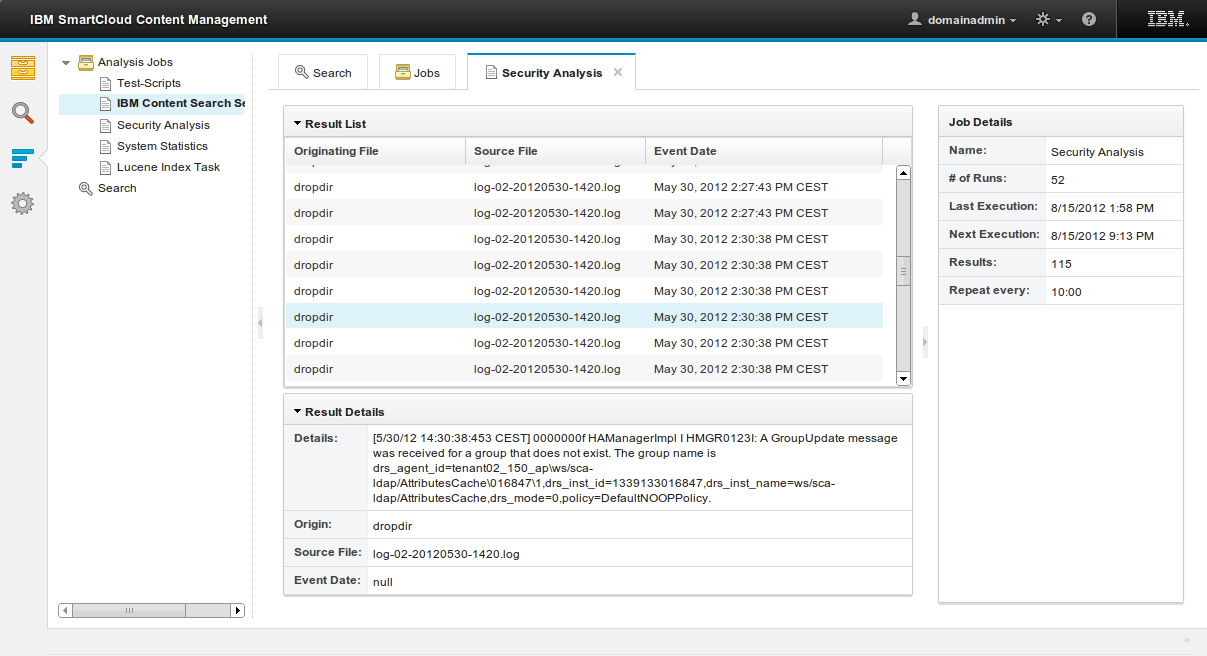
\includegraphics[width=16cm]{screens/job2.png}
	\caption{Screenshot of the log analysis plug--in UI}
	\label{fig:screenshot1}
\end{figure}

\subsection{Motivation}
As part of IBM's \ac{ecm} portfolio, \acl{sccm} is a \acl{saas} for document and email compliance archiving. It is a large integration project that makes use of many IBM software products, such as DB2\footnote{IBM DB2 is a relational database management system (DBMS).}, FileNet P8, \acl{was} and eDiscovery Manager\footnote{IBM \ac{edm} is an ECM product that finds documents related to a specific business case, for example a legal case, in a content repository.}, to provide an out--of--the--box archiving solution to customers. In this cloud environment, massive amounts of operational data are generated in the form of log files, especially if multiple customers are involved.

As \ac{ibm} is responsible for the operation of \ac{sccm}, problems have to be solved immediately as they arise, and steps must be taken to prevent problems beforehand. The large amounts of log data that the integrated software products generate contain knowledge that is necessary for \emph{predictive analysis}. Using IBM BigInsights, correlated log entries can be found and integrated to gain insights on the system's state and arising problems.

These analysis results have to be made available to the cloud operator in an easily accessable manner. Using Content Navigator to develop a front-end for the log analysis system not only makes it possible to integrate it with any ICN based product, but also emphasizes its ability to serve as a flexible, versatile web application framework.

The design and implementation of the BigInsights back-end are not in the scope of this thesis, as they mostly reflect the work of \citeasnoun{metzger}. Nevertheless the interface to the back-end --- a \ac{rest} service --- is presented, as it is essential to some functionality of the front-end.

\subsection{The REST service}
To create a log analysis plug--in and the according REST service, a basic understanding of the data being collected and shown must be present.

Robert Metzger built a data aggregating system using IBM \gls{biginsights}, which is a suite of different products related to \gls{bigdata} analysis. Metzger used different tools out of this suite to create two services: a full-text search for log files and a framework for data aggregation \emph{jobs}. These jobs can be defined using a powerful script language. They run periodically to collect log files, aggregate related log file entries and extract single information out of each collected entry.

Both these services are accessible via a REST service written in Java. The results of both are generated by the BigInsights system and are not meant to be manipulated or deleted by a user. For this reason, the REST service is read--only by design. Strictly spoken, this implementation of REST is incomplete, as there is no \emph{POST}, \emph{PUT} and \emph{DELETE} capability provided.

\subsubsection{Data format}
As the data format for the REST service, JSON was chosen. On the one hand, JSON is flexible without having a lot of overhead (compared to XML), on the other hand, it is natively supported by both the BigInsights products used and JavaScript (and Dojo, respectively). This makes it the preferable data format for this application scenario.

\subsubsection{Services}
The full-text search is available at the REST server's address at the URL \code{/search}. To initiate a query, the GET parameter ``query'' has to be provided with the according query string. A complete query for the string ``security'' looks like this: \code{127.0.0.1/search?query=security}, assuming the REST service runs on localhost\footnote{In IP networks, the IP \code{127.0.0.1} always refers to the \code{localhost}, the very one host that sends the request.}.

As a result, the search service sends a JSON array containing the found log entries as objects. Every object contains the source (the machine and service that wrote the log file), the entry's \gls{timestamp} and the exact log entry content.

The analysis jobs are accessed differently. The URL \code{/jobs} returns a list of all jobs that are known to the system. Besides other attributes, every job has a unique identifier which can be used to further access the job results via \code{/jobs/\%identifier\%}, where \code{\%identifier\%} has to be replaced with the according job identifier.

The list of jobs includes a description of every job. This description consists of metadata, such as the total number of collected results, as well as the structure of a result item. As every job can return completely different data, the client has to know the data structure, the type of every field (e.g. ``date'' or ``integer''), and if the field should be displayed or not. An example of a job description is given in the Appendix on page~\pageref{app:json}.

\subsubsection{Advanced features}
The REST service implements sorting and lazy loading. Both features are built to complement the client-side REST implementation of the \code{dojox.data.JsonRestStore}.

Lazy loading is a form of pagination. But instead of returning a certain ``page'' of data, the REST service returns a ``range''. This range is specified by GET parameters. The store on the client side keeps track of which items are already loaded. It then can request only those that are not loaded, but are needed to be displayed next.

Sorting is also implemented in the REST service on the server side. This may seem inconsequent in a Rich Client application, but it is necessary. Sorting can only be performed if all the data to be sorted are available. As the jobs can return more than 10.000 results, and not all results are loaded on the client due to lazy loading, it is unlikely that the client-side Model contains \emph{all} the items. Because the client would not be able to sort result items correctly if some are missing, sorting is implemented on the server instead.

\subsection{Implementation}
\label{sec:plugindesign}
This section gives a high-level overview on the architecture of the plug--in, especially on the MVC components. Exemplarily, one set of MVC components is presented in more detail.

The log analysis plug--in integrates into IBM Content Navigator and connects to the previously described REST service. The high-level architecture is shown in Figure~\ref{fig:loganalarch}.

\begin{figure}[H]
	\centering
	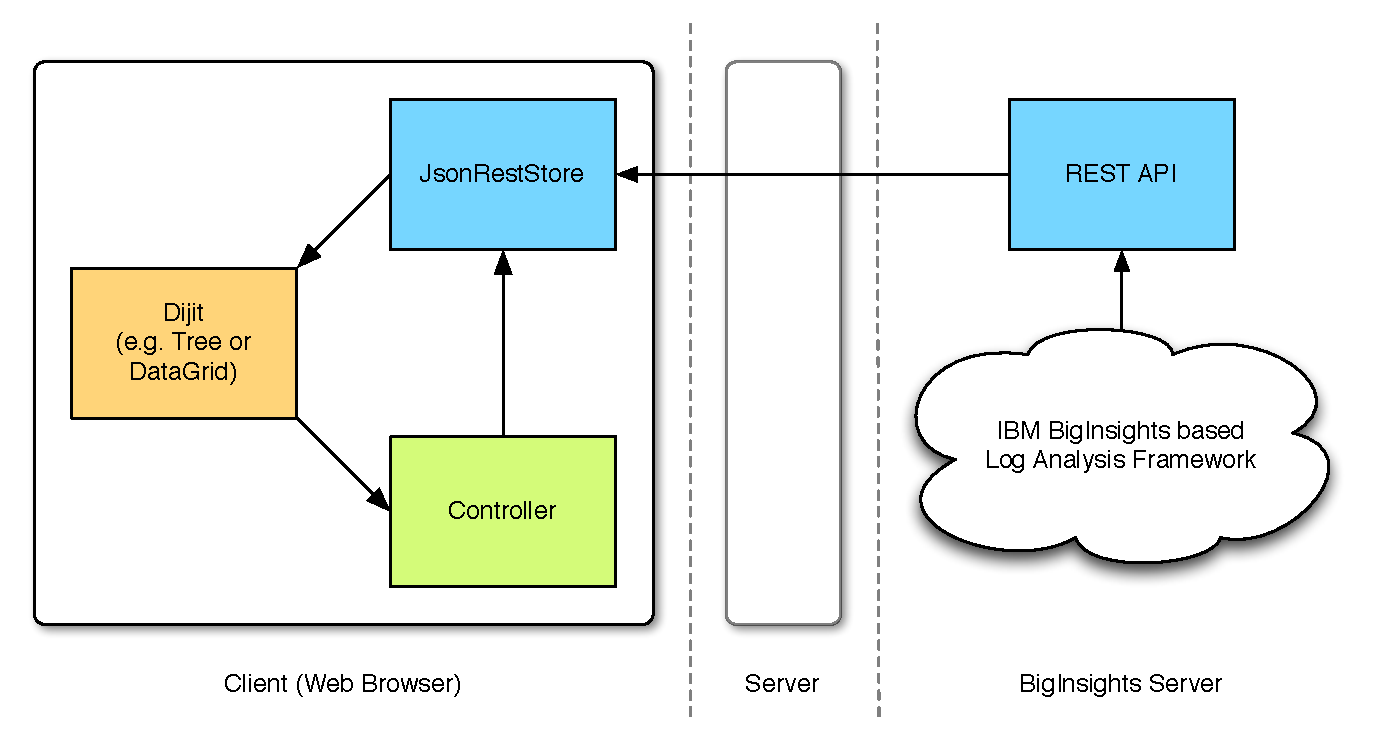
\includegraphics[width=14cm]{images/loganalarch.pdf}
	\caption{Integration of the log analysis plug--in into Content Navigator}
	\label{fig:loganalarch}
\end{figure}

\subsubsection*{File Structure}
The plug--in's \ac{jar} file contains a folder hierarchy, which on the top levels represents the Java package of the plug--ins. The path \pathname{/com/ibm/ecm/extension/sccm/} maps to the Java package \code{com.ibm.ecm.extension.sccm}. It contains two classes, the \code{SCCMPlugin} class, which represents the plug--in object within ICN and contains information on the plug--in components, and the \code{LogAnalysisFeature} class, which represents the \emph{Feature} that is exposed through the plug--in.

One level deeper, the \code{WebContent} folder contains the main \ac{css} and JavaScript files of the plug--in. \code{sccmPlugin.css} contains custom styles needed in the plug--in, while \code{sccmPlugin.js} loads the required Dojo classes using \code{dojo.require()} statements.

The folder hierarchy below \code{WebContent} can partially be mapped to JavaScript namespaces, but also contains additional resources:
\begin{description}
	\item[\code{sccm/layout}] contains Dijits used for layouting in the \code{sccm.layout} namespace
	\item[\code{sccm/model}] contains Models in the \code{sccm.model} namespace
	\item[\code{sccm/view}] contains Dijits used as Views in the \code{sccm.view} namespace
	\item[\code{sccm/resources}] contains images and \ac{css} files
\end{description}
The Dijits developed for the log analysis plug--in are based on \emph{\glspl{template}}, so every folder that contains Dijits also contains a \code{templates} folder with the according HTML files.

\code{sccm/ConfigurationPane.js} is a layout Dijit that gets included in the administration panel of ICN. It can be used to provide configuration options for the plug--in, such as the host and port of the log analysis REST service.

\begin{figure}
	\centering
	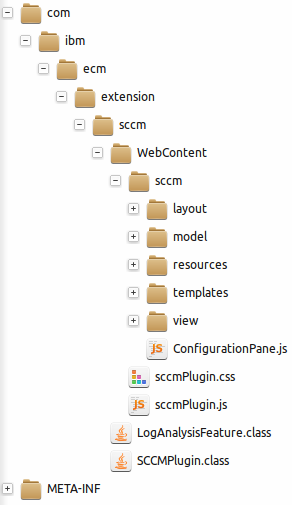
\includegraphics[width=6cm]{screens/folders.png}
	\caption{Folder hierarchy of the log analysis plug--in}
	\label{fig:folders}
\end{figure}

\subsubsection*{User Interface Integration and Layout}
To access the functionality of the log analysis plug--in, a new \emph{Feature} was created. When integrated into a Desktop, this Feature can be accessed using the Feature pane on the left side of the ICN interface.

The layout of the log analysis Feature was created using \emph{container Dijits}. These are Dijits that can themselves hold other Dijits, such as other container Dijits or Dijits that act as Views (i.e., display data).

\begin{description}
	\item[\code{sccm.layout.LayoutPane}] is the basic layout Dijit of the log analysis \emph{Feature}. It contains a \code{idx.layout.BorderContainer}, which divides the screen area into a left and right area. The left one is filled with a \code{dijit.Tree} to display all elements of the plug--in: the jobs overview, the full--text search and all existing jobs. Using this tree, the user can open the according Views in a tab. The right area of the LayoutPane holds a \code{dijit.layout.TabContainer} to display \emph{tabs}. Two tabs are initially included, containing the layout Dijits \code{sccm.layout.Search} and \code{sccm.layout.Overview}.
	\item[\code{sccm.layout.Search}] is a layout Dijit containing Views to perform the full--text search. It is instantiated inside the TabContainer of \code{sccm.layout.LayoutPane}, but could be used anywhere.
	The Search Dijit contains an input field and button to enter and submit the search term, as well as a \code{dojox.grid.DataGrid} to display the search results.
	\item[\code{sccm.layout.Overview}] contains a \code{sccm.view.StatsView} Dijit to display information on the state of the log analysis system, and a \code{sccm.view.JobsView} to list the Jobs that are registered with the system. The Overview Dijit is meant to be displayed inside a Tab in the TabContainer of \code{sccm.layout.LayoutPane}.
	\item[\code{sccm.layout.Messages}] is the only layout Dijit that is meant to be instantiated multiple times. It is used to display the details and results of a Job. For this reason, it contains a \code{sccm.view.DetailsView} for the Job details, as well as a \code{sccm.view.ResultsView} to list the results. A second \code{idx.grid.PropertyGrid} is used to display details for the selected result item.

	For every Job, there is one instance of \code{sccm.layout.Messages} opened as a tab, if the user double clicks the according job in the Job Overview tab or in the navigational tree on the left side of the \emph{Feature}.
\end{description}

\subsubsection*{Models}
In the log analysis plug--in, all Models (or Dojo stores, respectively) are created as Singletons\footnote{The Singleton is a design pattern which ensures that only one instance of an object exists at a given time. It is described by \citeasnoun[pp. 127--134]{gof}.}. This prevents access to the server-side Model from two different points in the application, which could cause memory leaks or lead to refetching of already fetched data.

Additionally to the data stores already provided by Dojo 1.6, it would have also been possible to create a custom one. The decision for \code{dojox.data.JsonRestStore} is explained below:
\begin{description}
	\item[ItemFileReadStore] The simple, read-only store \code{dojo.data.ItemFileReadStore} can use JSON as input, but expects a strict format\footnote{See \url{http://dojotoolkit.org/reference-guide/1.6/dojo/data/ItemFileReadStore.html}}, which is not feasible for the use case of a versatile REST API.
	\item[JsonRestStore] The \code{dojox.data.JsonRestStore} can be connected to a REST store and supports all CRUD\footnote{\emph{Create}, \emph{Read}, \emph{Update}, \emph{Delete}} actions through HTTP methods. Although the REST API does not have write capabilities, the JsonRestStore is the best match for the log analysis Models. All features that are required by our use case (and more) are supported by this store, for example the ability to request only a part of the data that is not already loaded; this is used to implement \emph{lazy loading}.
\end{description}

The namespace \code{sccm.model} contains all Models. The Model to manage the Job descriptions is instantiated as \code{sccm.model.Jobs}, whereas the search Model is created as \code{sccm.model.Search}.

The other Models, which hold the Job results, are instantiated when they are used for the first time. The object \code{sccm.model.messages} contains a method to initialize Models, which is shown in Listing~\ref{lst:models}. All Models of job results are managed as attributes of this object, identified by their unique job name.

\begin{figure}[H]
	\centering
	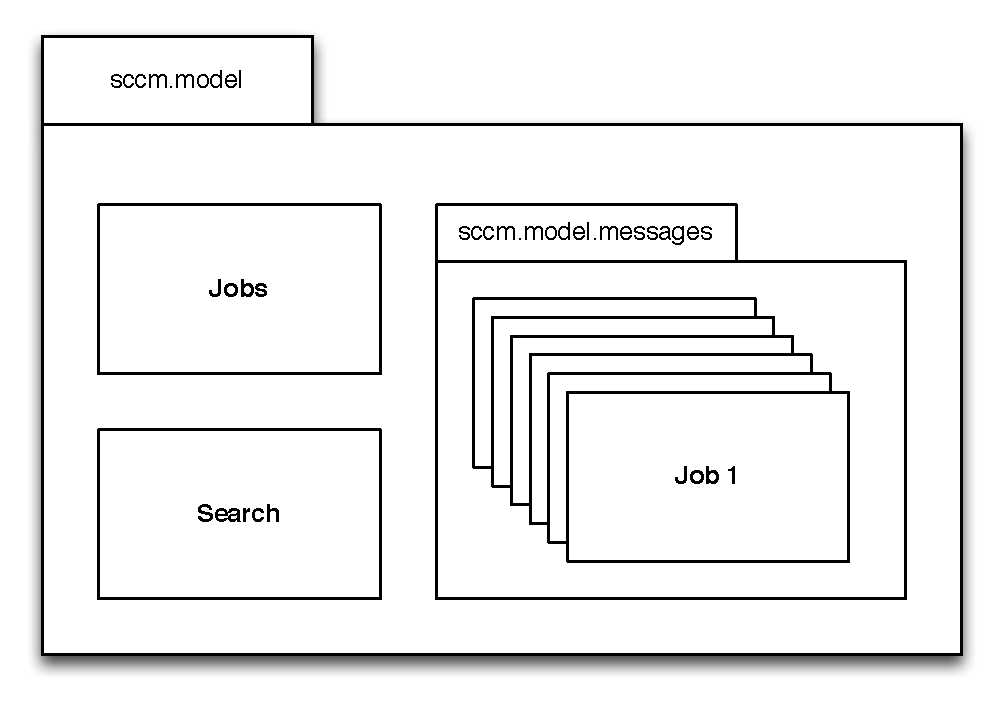
\includegraphics[width=12cm]{images/stores.pdf}
	\caption{Plug--in Models in the according namespaces}
	\label{fig:stores}
\end{figure}

\begin{listing}[H]
\begin{minted}[linenos=true,frame=none]{javascript}
sccm.model.messages = {
  getModel: function (name) {
    if(this[name] == undefined) {
      this[name] = new dojox.data.JsonRestStore({
        target: "http://9.152.130.251:8182/jobs/" + name
      });
    }
    return this[name];
  }
};
\end{minted}
\caption{Models for job results are created as Singletons}
\label{lst:models}
\end{listing}

An exemplary initialization of a results Model for the Job ``ibm-css'' is shown in Listing~\ref{lst:models2}. If the Model was not initialized before, it gets created then; otherwise, the reference to the existing Model is used.

\begin{listing}[H]
\begin{minted}[linenos=true,frame=none]{javascript}
theModel = sccm.model.messages.getModel('ibm-css');
\end{minted}
\caption{Initialization of a Model}
\label{lst:models2}
\end{listing}

\subsubsection*{Views and Controllers}
In the log-analysis plug--in, there is no View built completely from scratch. Although Dijits are \emph{visual} Dojo modules, they contain View code as well Controller code. These parts are hard to distinguish sometimes, as Dojo 1.6 does not provide a clearly structured MV* architecture.

As described in Section~\ref{sec:dojo}, the actual Views are Dijits such as \code{dijit.Tree} and \code{dojox.grid.DataGrid}. The log analysis plug--in does not extend or enhance them, it just \emph{uses} them.

The modules defined under the namespace \code{sccm.view} are not only Views, but View--Controller pairs. The Dijits, for example \code{sccm.view.StatsView}, are the Controllers, whereas the Views are defined inside their templates (or, programatically, inside the JavaScript code). In other words, the Controller \emph{wraps around} the View. This is the common way to define Dijits in \acl{icn}, as can be seen in the \emph{ICA Plug--in}, for example.

\begin{description}
	\item[\code{sccm.view.NavTree}] contains a \code{dijit.Tree} that displays all the plug--in's components. The search, jobs overview and job results can be accessed using this tree.
	The Controller code of this Dijit connects the Tree with the \code{sccm.model.Jobs} model
	\item[\code{sccm.view.StatsView}] is a Dijit containing an \code{idx.grid.PropertyGrid} (see Section~\ref{sec:customview} for more information on the PropertyGrid). It is used to the status of the log analysis system.
	\item[\code{sccm.view.JobsView}] contains a DataGrid to display the various log analysis jobs.
	\item[\code{sccm.view.ResultsView}] contains a DataGrid to display an overview of the job results.
	\item[\code{sccm.view.DetailsView}] contains a PropertyGrid to display details on a job result. This View is further described in Section~\ref{sec:customview}
\end{description}

\subsection{Implementation of a custom Model--View--Controller triad}
\label{sec:customview}
Part of the \ac{idx} distribution is a Dijit called \emph{PropertyGrid}. While the \emph{DataGrid} provided by stock Dojo is a good solution to get an overview on a large set of data, the \emph{PropertyGrid} is better suited to get a detailed view on a single object and its properties. In the log analysis plug--in, this was used in two places:
\begin{itemize}
	\item To display the properties of a \emph{Job} next to the list of results it returned,
	\item to display the system status and
	\item to display the details of the selected result item.
\end{itemize}
The last case is covered in this example. For every job, a \emph{tab} is created in a TabbedContainer Dijit (as described in Section~\ref{sec:plugindesign}) using the \code{sccm.layout.Messages} Dijit. The tab contains a DataGrid to display an overview of all the result items \code{sccm.view.ResultsView}, as well as a PropertyGrid to display details on the item that is \emph{selected} in the DataGrid \code{sccm.view.DetailsView}. Thus, the content of the PropertyGrid changes whenever a different item is selected in the DataGrid.
\begin{figure}[H]
	\centering
	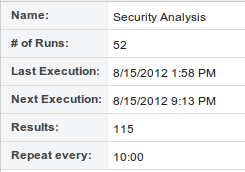
\includegraphics[width=6cm]{screens/propertygrid.png}
	\caption{The IDX PropertyGrid, displaying job details}
	\label{fig:propertygrid}
\end{figure}
Although the PropertyGrid is a data--driven Dijit, it is not designed to work together with a Dojo Store. The following example shows how this custom connection is established using the PropertyGrid as a View, a JsonRestStore through the DataGrid as a Model, and implementing Controller code to change the View's contents according to user actions.

One can argue that this is not a classic \ac{mvc} construction, as there is no Observer relationship between the View (\emph{PropertyGrid}) and the Model (the according \emph{JsonRestStore}). This is correct, but as the Model is read-only, the Observer is not necessary. It would be simple, though, to add it subsequently, if the PropertyGrid is used in a different scenario or the Model becomes writeable.

\subsubsection{Model}
The Model in this example is a simple \code{JsonRestStore}, as defined by Listing~\ref{lst:pgmodel}, but it is not used by the View directly. Instead, its data are accessed through the DataGrid, which is backed by the \code{JsonRestStore}. The listing defines a store for the ``ibm-css'' job. The \code{dataStructure} object is assumed to contain the structure for the DataGrid, which is not important here.
\begin{listing}[H]
\begin{minted}[linenos=true,frame=none]{javascript}
dataStore = new dojox.data.JsonRestStore({
  target: "http://localhost:8080/jobs/ibm-css"
});

dataGrid = new dojox.grid.DataGrid({
  store: dataStore,
  structure: dataStructure,
});
\end{minted}
\caption{Model and DataGrid for the PropertyGrid}
\label{lst:pgmodel}
\end{listing}

\subsubsection{View}
The PropertyGrid is created declaratively inside the template file of the tab.

\begin{listing}[H]
\begin{minted}[linenos=true,frame=none]{html}
<div
  dojoType="idx.grid.PropertyGrid"
  data="{}"
  properties=""
  dojoAttachPoint="detailsGrid"
></div>
\end{minted}
\caption{Declarative creation of the PropertyGrid}
\label{lst:pgview}
\end{listing}
Usually, the \code{data} attribute contains the data to be displayed, and the \code{properties} attribute contains information on how to format and label these data. In this case, both attributes are empty, as the information are set individually depending on the Model data.

\subsubsection{Controller}
As the Controller accesses two Dijits, it is placed one level higher, inside the \code{Messages.js} file of the \code{sccm.layout.Messages} Dijit. The code in Listing~\ref{lst:pgcontroller} is a simplified excerpt. It does not show the whole Dojo class developed for the tab of Job results, but only the parts relevant for the PropertyGrid. This code is also not in the context of the according Dojo class, but is extracted from it.

The code assumes a few objects to be present: \code{detailsGrid} is a reference to the PropertyGrid defined in Listing~\ref{lst:pgview}, \code{dataGrid} is a reference to the DataGrid, \code{job} contains the job description object (see Appendix and below).

The \code{structureForDetails()} function takes a \emph{result structure} object as the parameter. This object is part of the JSON description of a job; it describes the structure of a result item that is returned by an analysis job. In the Appendix, the JSON format of a job description is listed --- the \code{resultStructure} object, as part of it, is the object that gets passed in as a parameter here. \code{structureForDetails()} returns a string that lists all the properties that should be displayed in the PropertyGrid, and adds type information so that the properties are formatted properly. The returned string is in the format expected by the PropertyGrid for its \code{properties} attribute, as illustrated by Listing~\ref{lst:pgview}.

\code{detailsGrid} is a reference to the PropertyGrid Dijit. Using the \code{set()} method, the PropertyGrid's \code{properties} attribute is overwritten with a string created from the \emph{result structure} object, as described above.

The \code{dojo.connect()} function call in line~26 binds a callback, the \code{onRowClick()} function, to the \code{onRowClick} event of the DataGrid. This means, the callback is triggered when a row in the DataGrid is selected.

\code{onRowClick()} receives the selected result item from the DataGrid and sets it as the \code{data} attribute in the PropertyGrid. It then uses the \code{refreshPropertyGrid()} function to refresh the respective DOM nodes.

\begin{listing}[H]
\begin{minted}[linenos=true,frame=none]{javascript}
function structureForDetails(structure) {
  var a = "";
  for (var item in structure) {
    if(item != "__parent" && item != "__id") {
      var s = "";
      s = item;
      if(structure[item].type == "string")
        s += "(str)";
      else if(structure[item].type == "integer")
        s += "(int)";
      if(structure[item].type == "timestamp")
        s += "(dtm)";
      a += s + ",";
    }
  }
  // Remove trailing comma
  return a.substring(0,a.length - 1);
}

function onRowClick(event) {
  var item = dataGrid.getItem(event.rowIndex);
  detailsGrid.data = item;
  refreshPropertyGrid(this.detailsGrid);
}

function refreshPropertyGrid (pg) {
  for(var i = 0; i < pg._rows.length; i++)
    pg._rows[i].reformat();
}

// Set properties according to result structure
detailsGrid.set(
  "properties",
  structureForDetails(this.job.resultStructure)
);

dojo.connect(
  dataGrid,
  "onRowClick",
  dojo.hitch(this, onRowClick)
);
\end{minted}
\caption{Controller code for the PropertyGrid}
\label{lst:pgcontroller}
\end{listing}

\chapter{Conclusion, Reflection}\label{conclusion-reflection}


%\newpage
\newpage
\thispagestyle{empty}
\mbox{}
\newpage
 %neue Seite, damit Link auf Seitenanfang zeigt
%\phantomsection %notwendig, damit Link nicht unterhalb der Überschrift zeigt
%\addcontentsline{toc}{chapter}{Bibliography} %Eintrag im Inhaltsverzeichnis



\bibliographystyle{agsm}
\phantomsection
\setcounter{page}{1}
\pagenumbering{Roman}
\addcontentsline{toc}{chapter}{Bibliography}
\bibliography{ba}



\newpage
\setlength{\cftparskip}{-0.8pt}
\phantomsection
\addcontentsline{toc}{chapter}{List of Figures}
%\setlength\cftbeforechapskip{4pt}
%\setlength\cftbeforefigskip{4pt}
\listoffigures


\newpage
\thispagestyle{empty}
\mbox{}
\newpage
%\newpage
\phantomsection
\addcontentsline{toc}{chapter}{List of Tables}
\listoftables



\newpage
\listoflistings
\addcontentsline{toc}{chapter}{List of Listings}


\newpage
\printglossary{}

\chapter*{Appendix}
\renewcommand*{\chaptermarkformat}{}
\renewcommand*{\sectionmarkformat}{}
\chaptermark{Appendix}
\sectionmark{Appendix}
\addcontentsline{toc}{chapter}{Appendix}
\subsubsection*{Sample source code}
\label{app:diagram}
The following source code has been used for sketching during ideation and during prototyping.

\begin{listing}[H]
\begin{minted}[linenos=true,frame=none]{javascript}
;(function( window, document, $, undefined ) {
  console.log( this );
  $( document ).ready( function() {
    console.log( this );
    $('#btn').on('click', function( event ) {
      console.log( this );
      event.preventDefault();
      $.getJSON('document.json', function( data ) {
        console.log( this );
        data.forEach( function ( entry ) {
          console.log( this );
          $('#list').append('<li>' + entry.title + '</li>');
        });
      });
    });
  });
}( window, document, jQuery ));
\end{minted}
\caption{Sample client-side JavaScript program}
\label{lst:client}
\end{listing}

\begin{listing}[H]
\begin{minted}[linenos=true,frame=none]{javascript}
var fs = require('fs'),
    http = require('http'),
    marked = require('meta-marked'),
    handlebars = require('handlebars');

function parseMarkdown( cb ) {
  fs.readFile( 'article.md', function( err, data ) {
    if ( err ) {
      return cb( err );
    }

    var text = marked( data.toString() );
    cb( null, text );
  });
}

function compileHtml( text, cb ) {
  fs.readFile( 'template.html', function( err, data ) {
    if ( err ) {
      return cb( err );
    }

    var template = handlebars.compile( data.toString() );
    cb( null, template({
      meta: text.meta,
      content: text.html
    }) );
  });
}

var server = http.createServer( function( req, res ) {
  parseMarkdown( function( err, data ) {
    compileHtml( data, function( err, data ) {
      res.end( data );
    });
  } );
});

server.listen( 12345 );
\end{minted}
\caption{Sample server-side JavaScript program}
\label{lst:server}
\end{listing}


\end{document}
